\chapter{Синтез алгоритма буфера компенсации джиттера прибытия пакетов на основе робастного фильтра Калмана} \label{chapt3}

\section{Обзор алгоритмов фильтрации} \label{sect_analis_filters}


В стационарном состоянии сети задержка $x(t)$ представляет собой случайную величину, распределение вероятностей которой близкое к нормальному $N(0,\xi_x)$. 
Однако реальная статистика сети не является стационарной, как мы видим из второго раздела. Таким образом возникают флуктуации задержки, которые могут иметь как единичный характер так и продолжаться длительное время.
Все это приводит к тому, что плотность $p(x)$ нельзя считать идеально распределенной. 
Более того, реальную статистику, как правило, не удается параметризировать. Поэтому традиционные, хорошо разработанные параметрические процедуры для оценки задержки приминить сложно и рисковано. 
В этом случае имеет смысл перейти к непараметрическим робастным алгоритмам, которые хоть и не являются оптимальными, однако отличаются устойчивостью и при прочих равных условиях не проигрывают параметрическим.

Интерес к робастной обработке возник из осознания того факта, что исследователь никогда не располагает полными знаниями о действительной статистике.
Кроме того, предположение о гауссовом характере мешающих воздействий слишком идеализировано.
Как правило, мешающие воздействия имеют небольшой процент аномальных ``выбросов'', что приводит к утяжелению хвостов распределения. 
Эта статистическая неопределенность, а также наличие аномалий может быть учтена в модели ``засоренного'' распределения, предложенного Хьюбером \cite{huber}.

\begin{equation}\label{eq3:huber}
F(x)=(1-\varepsilon)F_0(x)+\varepsilon F_1(x),
\end{equation}
\noindent где $\varepsilon$ - небольшое положительное действительное число $(\varepsilon<0,1)$, $F_0(x)$ - известное распределение, $F_1(x)$ - распределение, принадлежащее некоторому классу, симметричное с конечной дисперсией.

Далее при построении алгоритма за оcнову взят принцип минимакса, т.е. алгоритм строится в рассчете на наименее благоприятное распределение.

Используем такой подход к построению алгоритма оценки процесса $S(\varphi)$. 
В качестве модели помех используем модель ``засоренного'' нормального распределения. 

\begin{equation}\label{eq3:kustov}
W(k)=(1-\varepsilon)N(0,\sigma)+\varepsilon N_1(0,\sigma_1),
\end{equation}

\noindent где $N(0,\sigma)$ и $N_1(0,\sigma_1)$ - нормальные распределения с нулевыми математическими ожиданиями и дисперсиями $\sigma$ и $\sigma_1$. 
Такая модель является наиболее характерной: составляющая $N_1$ описывает аномальную долю помех; составляющая $N$ прочие помехи, имещие вид гауссовых.

Тогда плотность совместного распределения аддитивной смеси сигнала и шума будет иметь вид:
\begin{equation}\label{eq3:kustov1}
W(V)=\frac{1-\varepsilon}{\sigma \sqrt{2\pi}}exp\frac{(V-S)^2}{2\sigma^2}+\varepsilon\frac{1}{\sigma_1\sqrt{2\pi}}exp\frac{(V-S)^2}{2\sigma_1^2},
\end{equation}

\noindent где $V=S(t)+n(t)$ - наблюдение процесса $S(\varphi)$.

Если наблюдение производится в дискретные моменты времени, то функция правдоподобия фазы $\varphi$ может быть записана в виде:

\begin{equation}\label{eq3:kustov2}
\begin{split}
L(\varphi)=&\prod_{i=1}^M \{(1-\varepsilon)\frac{1}{\sigma\sqrt{2\pi}}exp-\frac{[V_i-S_i(\varphi)]^2}{2\sigma^2}+\\
&+\varepsilon\frac{1}{\sigma_1\sqrt{2\pi}}exp-\frac{[V_i-S_i(\varphi)]^2}{2\sigma_1^2} \}.
\end{split}
\end{equation}

Для определения алгоритма оценки воспользуемся методом максимума функции правдоподобия \cite{tihonov}, т.е. в качестве оценки примем значение фазы $\hat{\varphi}$, являющейся решением уравнения:
\begin{equation}\label{eq3:kustov3}
\frac{dL}{d\varphi}/_{\varphi=\hat{\varphi}}=0.
\end{equation}

Подставим в уравнение (\ref{eq3:kustov3}) значение функции правдоподобия (\ref{eq3:kustov2}), получим уравнение:

\begin{equation}\label{eq3:kustov4}
\begin{split}
&\sum_{i=1}^M\left[\frac{V_i-S_i(\varphi)}{\sigma^2}\right]\frac{dS(\varphi)}{d\varphi}-\\
&-\sum_{i=1}^M\frac{\frac{\varepsilon}{1-\varepsilon}\frac{\sigma_1^2-\sigma^2}{\sigma_1^3\sigma}[V_i-S_i(\varphi)]\frac{dS_i(\varphi)}{d\varphi}exp\left\{\frac{\sigma_1^2-\sigma^2}{2\sigma_1^2\sigma^2}[V_i-S_i(\varphi)]\right\}}{1+\frac{\varepsilon}{1-\varepsilon}exp\left\{\frac{\sigma_1^2-\sigma^2}{2\sigma_1^2\sigma^2}[V_i-S_i(\varepsilon)]^2\right\}}=0.
\end{split}
\end{equation}

Типичным для практики являются следующие значения величин: $\varepsilon\leq0,1$ и $\sigma_1\geq10\sigma$.

Рассмотрим вторую сумму. Если $V_i\geq3\sigma_1$, то единицей в знаминателе можно пренебречь и тогда этот член в сумме имеет вид:
\begin{equation}\label{eq3:kustov5}
\frac{1}{\sigma^2}[V_i-S_i(\varphi)]\frac{dS(\varphi)}{d\varphi},
\end{equation}
\noindent т.е. равен соответствующему члену первой суммы, а их разность равна 0, т.е. в оптимальном алгоритме при обработке эти члены не учитываются.

Если $V_i\leq3\sigma$, то вторым членом в знаминателе второй суммы можно пренебречь по сравнению с единицей. Числитель второй суммы будет иметь значение $\leq0,01$ и этими состовляющими первой суммы можно пренебречь.

Рассмотренная процедура оценки является точечной, привязанной к конкретной ситуации. В этой процедуре, не учитывается предистория и не используется экстраполяция, что для решений сетевых задач имеет принципиальное значение. 
Очевидно, можно создать процедуру, состоящую из последовательности точечных оценок в каждой из временных позиций по алгоритму (\ref{eq3:kustov4}).
Но данная процедура не ориентирована на учет параллельных связей между соседними позициями $i$ и $i+1$.

Применим более общую марковскую модель функционирования сети, при которой соседние позиции связаны соотношением:
\begin{equation}\label{eq3:kustov6}
x(i+1)=P(x_{i+1}/x_i)x(i),
\end{equation}
\noindent где $P(x_{i+1}/x_i)$ - вероятность перехода, представляющая по сути коэффициент изменения между указанными позициями процесса $x(i)$.

Выбор модели (\ref{eq3:kustov6}) позволяет построить рекурсивную процедуру, как самой модели состояния процесса $x(i)$, так и алгоритма оценки в виде фильтра Калмана-Бьюси или в виде более простой процедуры стохастической апроксимации.










Фильтр Калмана-Бьюси дает решение задачи оптимального оценивания в линейных динамических системах при гауссовском распределение помех.
Однако в нашей прикладной задаче, распределение шумов не является гауссовским, причем распространенной причиной отклонения распределения вероятностей помех от гауссовского является наличие выбросов и скачков в оцениваемом процессе.
Хорошо известно \cite{cipkin}, что такие отклонения существенно ухудшают качество оценок, получаемых с помощью алгоритмов, оптимальных для гауссовских помех.
Поэтому не случайно большое внимание удуляется разаработке робастных алгоритмов фильтрации, стабильно работающих в условиях, когда помехи содержат выбросы или скачки \cite{Klekis, masreliez_ieee, masreliez_martin, ershov_lipcer, ershov, RobustFilter}.
В \cite{masreliez_ieee} задача фильтрации при наличие выбросов решалась, как задача   негаусовской фильтрации, однако реализация полученного алгоритма на ЭВМ представляет затруднительные трудности. 
Дальнейшее развитие этот подход получил в \cite{masreliez_martin}. Однако этот алгоритм фильтрации имеет ряд недостатков: для его построения необходимо знать вероятность появления выброса и распределение вероятностей помех должно быть симметричным. Данный подход не подходит для решения нашей задачи, так как задержка в телекоммуникационных системах является нестационарной.

Другой подход к решению задачи фильтрации помех, содержащих выбросы, представлен в \cite{ershov_lipcer, ershov}. В представлении шумов предполагается, что с большей вероятностью помехи измерения распределены нормально с нулевым средним и заданной ковариационной матрицей и с малой вероятностью распределны также нормально,  но с ковариационной матрицей, имеющей большую норму. Алгоритм фильтрации основан на обнаружении момента появления выброса и изменении коэффициента усиления в зависимости от результатов обнаружения. Для модификации коэффициента используется ковариационная матрица источников выбросов.

В \cite{Klekis} предполагается, что в нормальном режиме работы измерительного устройства помехи распределены нормально с нулевым средним и известной ковариационной матрицей, а в режиме сбоев помехи имеют нормальное распределение с неизвестным средним и той же ковариационной матрицей.
Алгоритм фильтрации получен на основе обнаружения момента появления выброса, оценивания его амплитуду и соответственно модифицируя коэффициент усиления и ковариационную матрицу. В этом случае априорной информации о характеристиках выбросов не требуется.  

Рассмотрим более детально алгоритмы фильтрации описанные выше:

\textbf{1. Фильтр Калмана (ФК).}
 ФК синтезирован с учетом того, что наблюдаемый процесс соответствует уравнению (\ref{eq3:modelStat}) и наблюдается на фоне гауссовского белого шума.
 Уравнение оценки в виде условного среднего значения задержки с использованием ФК имеет вид:


\begin{equation}\label{eq3:Estim_rel}
\hat{x}(k+1)=\Phi\hat{x}(k)+K(k)\Delta y,
\end{equation}
\noindent где $\Delta y=H\Phi\hat{x}(k)-y(k)$ - невязка, $K(k)$ - коэффициент, обеспечивающий устойчивость и сходимость процедуры, в частности $K(k)$ может быть константой $K\leq1$. Коэффициент усиления ФК $K(k)$ является функцией от апостериорной дисперсии ошибки оценки $V(k)$, что ускоряет его сходимость:

\begin{equation}\label{eq3:K}
K(k)=V(k)H^TN_{\nu}^{-1},
\end{equation}
 
\begin{equation}\label{eq3:V}
V(k)=[I-K(k-1)H(k)]V(k,k-1),
\end{equation}


\begin{equation}\label{eq3:Vkk-1}
V(k,k-1)=\Phi^TV(k-1)\Phi+N_\xi,
\end{equation}

\noindent где $V(k)$ - апостериорная дисперсия ошибки оценки, $V(k,k-1)$ - априорная дисперсия ошибки оценки, $I$ - единичная матрица.

На рис. \ref{img3:kalmanF} представлена схема сглаживающего фильтра, построенная в соответствии с (\ref{eq3:Estim_rel}). Ключевую роль в оценке ФК текущего значения задержки, является параметр $\Phi$ позволяющий регулировать сглаживающие свойства фильтра. 

\begin{figure} [h]
  \center
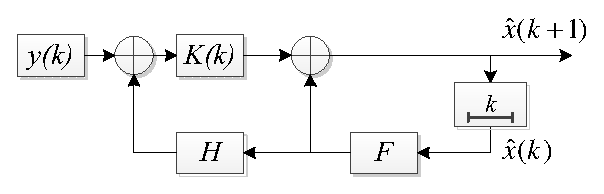
\includegraphics[width=0.8\textwidth]{3chapter/10.eps}
  \caption{Схема ФК}
  \label{img3:kalmanF}
\end{figure}


\textbf{2. Алгоритм фильтрации, который может быть синтезирован в том случае, когда в (\ref{eq3:v}), (\ref{eq3:vp}) известны последовательности $\mathbf{\{r_v\}}$, $\mathbf{\{R_2(k)\}}$.} Выражения описывающие алгоритм, имеют вид:

\begin{equation}\label{eq3:optim2}
\hat{x}(k+1)=\Phi\hat{x}(k)+K(k)\Delta y,
\end{equation}

\begin{equation}\label{eq3:optim2_3}
V(k|k-1)=\Phi(k-1)V(k-1)\Phi^T(k-1)+N_\xi,
\end{equation}

\begin{equation}\label{eq3:optim2_4}
\begin{split}
K(k)=&V(k|k-1)H^T(k)\{H(k)V(k|k-1)H^T(k)+\\
&+[1-r_v(k)R_1(k)+r_v(k)R_2(k)\}^{-1},
\end{split}
\end{equation}

\begin{equation}\label{eq3:optim2_5}
V(k)=[I-K(k-1)H(k)]V(k,k-1).
\end{equation}

\textbf{3. Алгоритм фильтрации при известной верояности появления выбросов $\mathbf{\varepsilon}$ и известных ковариационных матрицах $\mathbf{\{R_2(k)\}}$:}

\begin{equation}\label{eq3:optim3}
\hat{x}(k+1)=\Phi\hat{x}(k)+K(k)\Delta y,
\end{equation}

\begin{equation}\label{eq3:optim3_3}
V(k|k-1)=\Phi(k-1)V(k-1)\Phi^T(k-1)+N_\xi,
\end{equation}

\begin{equation}\label{eq3:optim3_4}
\begin{split}
K(k)=&V(k|k-1)H^T(k)[H(k)V(k|k-1)H^T(k)+\\
&+(1-\varepsilon)R_1(k)+\varepsilon R_2(k)]^{-1},
\end{split}
\end{equation}

\begin{equation}\label{eq3:optim3_5}
V(k)=[I-K(k-1)H(k)]V(k,k-1).
\end{equation}

\textbf{4. Алгоритм фильтрации с оценкой выбросов, требующий информацию о характеристиках выбросов:}

\begin{equation}\label{eq3:optim4}
\hat{x}(k+1)=\Phi\hat{x}(k)+K(k)\Delta y,
\end{equation}

\begin{equation}\label{eq3:optim4_3}
V(k|k-1)=\Phi(k-1)V(k-1)\Phi^T(k-1)+N_\xi,
\end{equation}

\begin{equation}\label{eq3:optim4_4}
\begin{split}
K(k)=&V(k|k-1)H^T(k)\{H(k)V(k|k-1)H^T(k)+\\
&+(1-\hat{r}_v(k))R_1(k)+\hat{r}_v(k)R_2(k)\}^{-1},
\end{split}
\end{equation}

\begin{equation}\label{eq3:optim4_5}
\begin{split}
V(k)=&[I-K(k-1)H(k)]V(k,k-1)[I-K(k-1)H(k)]^T+\\
&+K(k)R_1(k)K^T(k).
\end{split}
\end{equation}

\begin{equation}
\hat{r}_v(k)= \;
\begin{cases}
0, \; ||\Delta y(k)||\leq c_1 \\    
1, \; ||\Delta y(k)||> c_1    
\end{cases}
\end{equation}

\textbf{5. Алгоритм фильтрации, не требующий информации о вероятности появления и амплитудах выбросов.} Алгоритм использует следующую модель помех:
\begin{equation}\label{eq3:optim5_01}
\xi(k)=\xi(k)+r_v(k)Bu(k),
\end{equation}
\begin{equation}\label{eq3:optim5_01}
P[\xi(k)]=(1-\varepsilon)N[0,R_1(k)]+\varepsilon N[Bu(k),R_1(k)],
\end{equation}
\noindent где $u(k)$ - неизвестный, неслучайный вектор, $B$ - известная матрица соответствующих размеров.
\begin{equation}\label{eq3:optim5}
\hat{x}(k+1)=\Phi\hat{x}(k)+[1-\hat{r}_v(k)BL(k)]K(k)\Delta y,
\end{equation}

\begin{equation}\label{eq3:optim5_1}
L(k)=[B^TVv^{-1}(k)B]^{-1}B^TV^{-1}(k),
\end{equation}

\begin{equation}\label{eq3:optim5_2}
Vv(k)H(k)V(k,k-1)H^T(k)+R_1(k),
\end{equation}

\begin{equation}\label{eq3:optim5_3}
V(k|k-1)=\Phi(k-1)V(k-1)\Phi^T(k-1)+N_\xi,
\end{equation}

\begin{equation}\label{eq3:optim5_4}
K(k)=V(k|k-1)H^T(k)[H(k)V(k|k-1)H^T(k)+R_1(k)]^{-1},
\end{equation}

\begin{equation}\label{eq3:optim5_5}
\begin{split}
V(k)=&[I-K(k-1)H(k)]V(k,k-1)[I-K(k-1)H(k)]^T+\\
&+K(k)R_1(k)K^T(k)+\hat{r}_vK(k)BD(k)B^TK^T(k),
\end{split}
\end{equation}

\begin{equation}\label{eq3:optim5_6}
D(k)=[B^TV^{-1}(k)B]^{-1},
\end{equation}

\begin{equation}\label{eq3:optim5_7}
\hat{r}_v(k)= \;
\begin{cases}
0, \; ||l(k)||\leq c_2 \\    
1, \; ||l(k)||> c_2    
\end{cases}
\end{equation}

\begin{equation}\label{eq3:optim5_8}
l(k)=\Delta y^TV^{-1}(k)B[B^TV^{-1}(k)B]^{-1}B^TV^{-1}(k)\Delta y,
\end{equation}

Из анализа этих алгоритмов \cite{Klekis} отметим что алгоритмы (\ref{eq3:optim4})-(\ref{eq3:optim4_5}) и (\ref{eq3:optim5})-(\ref{eq3:optim5_8}) уступают по точности второму алгоритму фильтрации, но дают более точные оценки, чем ФК.
Особенно это характерно в случае мощных выбросов.
По точности алгоритмы (\ref{eq3:optim4})-(\ref{eq3:optim4_5}) и (\ref{eq3:optim5})-(\ref{eq3:optim5_8}) различаются незначительно, однако в отличии от первого второй не требует информации о характеристиках выбросов

\begin{table} [h]
  \centering
  \parbox{15cm}{\caption{Дисперсия ошибок оценивания в момент $k=20$. $\sigma_{OPT}^2$ - для оптимального фильтра (\ref{eq3:optim2})-(\ref{eq3:optim2_5}), $\sigma_{LIN}^2$ - для линейного фильтра (\ref{eq3:optim3})-(\ref{eq3:optim3_5}), $\sigma_{KAL}^2$ - для ФК, $\sigma_{RB1}^2$ - для алгоритма (\ref{eq3:optim4})-(\ref{eq3:optim4_5}), $\sigma_{RB2}^2$ - для алгоритма (\ref{eq3:optim5})-(\ref{eq3:optim5_8}) \cite{Klekis}} \label{disp_opt}} 
\begin{center}
\begin{tabular}{|l|l|l|l|l|l|l|l|} \hline \hline
$R_1=1$ & $\varepsilon$ & $R_2$ & $\sigma_{OPT}^2$ & $\sigma_{LIN}^2$ & $\sigma_{KAL}^2$ & $\sigma_{RB1}^2$ & $\sigma_{RB2}^2$\\\hline \hline
0,1 & 0,05 & 9 & 0,210 & 0,247 & 0,248 & 0,232 & 0,234\\\hline \hline
0,1 & 0,05 & 36 & 0,211 & 0,314 & 0,367 & 0,222 & 0,222\\\hline
0,1 & 0,05 & 100 & 0,211 & 0,386 & 0,655 & 0,223 & 0,223\\\hline
0,1 & 0,2 & 9 & 0,234 & 0,308 & 0,381 & 0,287 & 0,291\\\hline
0,1 & 0,2 & 36 & 0,235 & 0,410 & 0,921 & 0,277 & 0,273\\\hline
0,1 & 0,2 & 100 & 0,235 & 0,469 & 2,182 & 0,263 & 0,262\\\hline
1 & 0,05 & 9 & 0,633 & 0,748 & 0,782 & 0,744 & 0,746\\\hline
1 & 0,05 & 36 & 0,638 & 1,129 & 1,391 & 0,763 & 0,761\\\hline
1 & 0,05 & 100 & 0,639 & 1,697 & 2,823 & 0,770 & 0.761\\\hline
1 & 0,2 & 9 & 0,792 & 1,093 & 1,332 & 1,066 & 1,072\\\hline
1 & 0,2 & 36 & 0,829 & 1,951 & 3,659 & 1,377 & 1,407\\\hline
1 & 0,2 & 100 & 0,835 & 2,861 & 9,156 & 1,258 & 1,286\\\hline
\end{tabular}
\end{center}
\end{table}

Рассмотренные алгоритмы обладают рядом недостатков:
\begin{enumerate}
 \item Алгоритм ФК дает решение оптимального оценивания в линейных динамических системах при гауссовском распределение помех, а при отклонении от норамального распределения (выбросы и скачки) качество оценивания существенно ухудшаются.
 \item Для реализации 2-4 алгоритмов необходима априорная информация о характеристиках выбросов, а так как телекоммуникационные системы нестационарны, то практическое применение этих алгоритмов в таких системах ограничено.
 \item Ни один алгоритм не учитывает особенностей, которые необходимо учитывать при фильтрации случайного процесса содержащего скачки.
\end{enumerate}
Для решения этих недостатков рассмотрим ряд робастных алгоритмов фильтрации из \cite{RobustFilter}.

\section{Обзор робастных алгоритмов фильтрации на основе фильтра Калмана для случайных процессов содержащих выбросы и скачки} \label{sect3_grfk}

\textbf{1. Алгоритм РФК для случайного процесса, содержащего выбросы,} согласно \cite{RobustFilter} выглядит следующим образом:

\begin{equation}\label{eq3:skachok}
\hat{x}(k+1)=\Phi(k+1,k)\hat{x}(k)+K(k)\Delta y\cdot min\left\{1,\frac{b}{|K(k)\Delta y|}\right\},
\end{equation}

\noindent где $b$ является некоторым ограничителем изменения значения функции. 
Это позволяет решить проблему неограниченого изменения оценки за один шаг в классическом фильтре Калмана, оставаясь при этом достаточно простой.

Если $b\geq |K(k) \Delta y |$, то $min\left\{1,\frac{b}{|K(k)\Delta y|}\right\}$ принимает значение 1 и фильтр работает в обычном режиме как ФК (\ref{eq3:Estim_rel}). Если же $b\leq |K(k) \Delta y |$, то из этого следует, что произошел выброс и невязка умножается на понижающий коэффициент, равный $\frac{b}{|K(k)\Delta y|}$, что опять же приводит РФК к обычному виду (\ref{eq3:Estim_rel}).


\textbf{2. Алгоритм РФК для случайного процесса, содержащего скачки,} согласно \cite{RobustFilter} выглядит следующим образом:

\begin{equation}\label{eq3:vibros}
\begin{split}
\hat{x}(k+1)=&\Phi(k+1,k)\hat{x}(k)+H(k)[I-H(k)K(k)\Delta y]\times \\
&\times min\left\{1,\frac{b}{|I-H(k)K(k)\Delta y|}\right\},
\end{split}
\end{equation}

\noindent где $b$ тот же аргумент, ограничивающий изменение значения функции, что и для РФК для ситуации выброса (\ref{eq3:skachok}).

\textbf{3. Гибридный робастный фильтр Калмана (ГРФК)}

Очевидно, одновременная фильтрация возможна только с некоторой задержкой $\Delta \tau$. 
Это необходимо для принятия решения о типе отклонения от нормального распределения. 
Вследствие выброса скорей всего увидим один большой выброс (\ref{eq3:v}), а вследствие скачка – подряд целую последовательность (\ref{eq3:s}). 
ГРФК может быть реализован следующим образом \cite{RobustFilter}: РФК для случайного процесса с выбросами работает по умолчанию и всякий раз, когда ширина выброса больше, чем окно наблюдения $\Delta \tau$, единожды используется процедура РФК для случайных процессов со скачками.



\section{Сравнительный аналих алгоритмов фильтрации для случайных процессов содержащих выбросы и скачки} \label{sect3_6}
Чтобы сравнить алгоритмы фильтрации проведем моделирование оценки случайного процесса с помощью приведенных робастных алгоритмов фильтрации и фильтра Калмана. Результаты приведены на рис. \ref{img3:filterIdeal}-\ref{img3:filterMix}. Сплошной линией со снежинками показан наблюдаемый процесс, сплошной – оценка ФК, штрихпунктирной с точками – РФК для ситуации с выбросами, штрихпунктирной - РФК для ситуации со скачками и штрихпунктирной со снежинками – ГРФК. На рис. \ref{img3:filterIdeal} представлены результаты оценивания временного процесса без выбросов и скачков (\ref{eq3:Estim}), из графика следует, что рассмотренные робастные алгоритмы, не теряют своей оптимальности по сравнению с ФК, во время оценивания процесса без выбросов и скачков.
На рис. \ref{img3:filterVibros} представлены результаты оценивания временного процесса с выбросами (\ref{eq3:v}), из графика следует, что РФК для ситуации выброса и ГРФК позволяют игнорировать выбросы, что обеспечивает оптимальную оценку процесса.
На рис. \ref{img3:filterSkachok} представлены результаты оценивания временного процесса со скачками (\ref{eq3:v}), из графика следует, что РФК для ситуации скачка и ГРФК позволяют быстро переключиться на новое значение задержки. В то время как РФК для ситуации выброса оказался не в состоянии отслеживать скачки.
В заключение, на рис. \ref{img3:filterMix} представлены результаты оценивания временного процесса со скачками и с выбросами, из графика следует, что, ГРФК позволяет получить оптимальную оценку в смешанной ситуации, в то время как остальные алгоритмы выполняют оценку недопустимо плохо.


\pgfplotsset{width=15cm, height=10cm, compat=1.3}
\begin{figure} [h]
  \center
\begin{tikzpicture}
%\pgfkeys{/pgfplots/legend pos=north west}

\begin{axis}[
mark options={scale=0.5},
ylabel={Mem [GB]},
legend style={
%area legend,
at={(0.5,-0.20)},
anchor=north,
legend columns=3},
legend cell align=left,
cycle list name=mark list,
%cycle list name=linestyles,
xlabel=Порядковый номер пакета,
ylabel=Задержка (мс),
xmin=200,
xmax=300
]

				\addplot coordinates {
					(1, 20.0)
					(2, 20.2863761931)
					(3, 19.982683057)
					(4, 19.5220644)
					(5, 19.602464332)
					(6, 20.0234570071)
					(7, 19.8444577633)
					(8, 20.0522938721)
					(9, 19.4870140232)
					(10, 19.6096931395)
					(11, 19.2741416091)
					(12, 19.4813472933)
					(13, 19.2676345646)
					(14, 19.3829283545)
					(15, 19.0639958809)
					(16, 18.9824859016)
					(17, 19.0669442068)
					(18, 18.395363523)
					(19, 17.7522189906)
					(20, 17.7434389634)
					(21, 17.4845561771)
					(22, 17.3158790057)
					(23, 17.2286771582)
					(24, 17.2747261135)
					(25, 16.7074723756)
					(26, 16.4220508477)
					(27, 16.4004137946)
					(28, 16.0249203381)
					(29, 16.3753623217)
					(30, 15.9681916175)
					(31, 16.4733744175)
					(32, 16.9327544208)
					(33, 17.3043239281)
					(34, 17.1096192347)
					(35, 17.3240267918)
					(36, 17.0345899915)
					(37, 17.0597628178)
					(38, 17.0666625084)
					(39, 16.7854376433)
					(40, 16.574047305)
					(41, 17.0121522318)
					(42, 16.8125393599)
					(43, 16.7382063936)
					(44, 16.6971721155)
					(45, 16.859596165)
					(46, 16.8699178963)
					(47, 16.802136803)
					(48, 16.6967974268)
					(49, 16.1423810366)
					(50, 16.3604911237)
					(51, 16.3978185226)
					(52, 15.8141959566)
					(53, 15.8860425711)
					(54, 16.1817026098)
					(55, 16.3687037)
					(56, 16.643399307)
					(57, 16.8846000846)
					(58, 16.7949196988)
					(59, 17.0448689651)
					(60, 17.1779420485)
					(61, 17.4443981059)
					(62, 17.6747513432)
					(63, 17.8722152408)
					(64, 18.0543467739)
					(65, 18.1593826661)
					(66, 18.294272557)
					(67, 18.739801523)
					(68, 18.50801733)
					(69, 18.0912334095)
					(70, 18.4579205411)
					(71, 18.3053580785)
					(72, 18.7181262387)
					(73, 18.5636424372)
					(74, 18.1529316436)
					(75, 18.2528409043)
					(76, 17.9109607273)
					(77, 17.9171188298)
					(78, 18.0943144555)
					(79, 17.8544265551)
					(80, 18.0917256864)
					(81, 18.3317646042)
					(82, 17.7810213343)
					(83, 18.0385463971)
					(84, 17.6295317874)
					(85, 17.6414430776)
					(86, 17.7693978162)
					(87, 17.7994816094)
					(88, 17.8605008437)
					(89, 17.9838426835)
					(90, 17.8627595476)
					(91, 17.6054025027)
					(92, 17.6210579243)
					(93, 17.6296333059)
					(94, 17.4920272732)
					(95, 16.921074956)
					(96, 16.7904335669)
					(97, 16.2690891767)
					(98, 16.059869209)
					(99, 16.1676018071)
					(100, 16.3132101865)
					(101, 16.3428529337)
					(102, 16.6366372593)
					(103, 16.5324983983)
					(104, 16.5728104285)
					(105, 16.6451859592)
					(106, 16.9307264605)
					(107, 16.9091459317)
					(108, 17.3470671251)
					(109, 17.0780154184)
					(110, 17.0547464898)
					(111, 16.4871055119)
					(112, 16.508836767)
					(113, 16.991659316)
					(114, 16.7680234775)
					(115, 16.7431786939)
					(116, 16.9448075955)
					(117, 17.347433714)
					(118, 17.1738869179)
					(119, 17.0124306248)
					(120, 17.159526132)
					(121, 17.5875202866)
					(122, 18.0662753327)
					(123, 17.5916250086)
					(124, 18.380710759)
					(125, 18.4641226547)
					(126, 18.2548730663)
					(127, 17.9624168529)
					(128, 17.6645052785)
					(129, 17.6069603679)
					(130, 18.0400635262)
					(131, 18.2951906595)
					(132, 17.9038004167)
					(133, 18.0896310554)
					(134, 17.8822605037)
					(135, 17.4653347242)
					(136, 17.277643091)
					(137, 17.5679831501)
					(138, 17.6258097063)
					(139, 17.4744234005)
					(140, 17.929215196)
					(141, 18.1460447592)
					(142, 17.8965270149)
					(143, 18.2630609013)
					(144, 18.4246993197)
					(145, 18.4158493432)
					(146, 18.6018070044)
					(147, 18.905966958)
					(148, 19.1388698019)
					(149, 19.1631100719)
					(150, 18.8265096274)
					(151, 18.6454001939)
					(152, 18.875347641)
					(153, 18.7760784217)
					(154, 19.2297090714)
					(155, 19.5247428091)
					(156, 19.3382428276)
					(157, 19.2214358765)
					(158, 19.1073386484)
					(159, 18.887708243)
					(160, 18.9687622294)
					(161, 18.9718669304)
					(162, 19.1201918458)
					(163, 19.11441939)
					(164, 18.729571742)
					(165, 19.0424482165)
					(166, 19.1659891933)
					(167, 19.0391218497)
					(168, 18.6152886826)
					(169, 18.641669865)
					(170, 18.8131817708)
					(171, 19.0973486079)
					(172, 18.9987752671)
					(173, 18.6973710231)
					(174, 19.0235606726)
					(175, 18.9641061842)
					(176, 18.7936069731)
					(177, 18.8236812953)
					(178, 18.5686080116)
					(179, 18.721031714)
					(180, 18.8601586297)
					(181, 19.3523863173)
					(182, 19.0314870658)
					(183, 18.469278548)
					(184, 19.0191709841)
					(185, 18.9237974944)
					(186, 19.6461698738)
					(187, 19.6628458835)
					(188, 19.8058528547)
					(189, 19.8284387206)
					(190, 19.6893911911)
					(191, 19.7220796636)
					(192, 19.5085331658)
					(193, 19.3202934795)
					(194, 19.5049196502)
					(195, 19.4449262415)
					(196, 19.0140957401)
					(197, 19.0901699563)
					(198, 18.9551157296)
					(199, 19.1996245464)
					(200, 19.6436038737)
					(201, 19.4370031259)
					(202, 19.6316051302)
					(203, 19.4178484356)
					(204, 18.9002333968)
					(205, 18.8611845737)
					(206, 18.6090058581)
					(207, 18.368943845)
					(208, 18.1133432089)
					(209, 18.5632757055)
					(210, 18.6941705727)
					(211, 19.0713237147)
					(212, 19.073026226)
					(213, 19.5099637474)
					(214, 18.9835359368)
					(215, 18.5593445906)
					(216, 18.8724148839)
					(217, 19.2611352682)
					(218, 18.7753109378)
					(219, 18.5938378483)
					(220, 18.7593703709)
					(221, 18.4669663863)
					(222, 18.3633885993)
					(223, 18.5271877046)
					(224, 18.395827221)
					(225, 18.1372593594)
					(226, 18.3118247588)
					(227, 18.3740304867)
					(228, 18.8638970345)
					(229, 19.1296758318)
					(230, 19.1880277631)
					(231, 19.3069271752)
					(232, 19.7596388511)
					(233, 20.1895066843)
					(234, 20.5589058793)
					(235, 20.8278952656)
					(236, 20.3087990794)
					(237, 20.3923939639)
					(238, 20.2820797191)
					(239, 20.2061717945)
					(240, 20.2177813569)
					(241, 19.8011350594)
					(242, 19.6177988144)
					(243, 19.7362901677)
					(244, 19.8018075618)
					(245, 19.9319777218)
					(246, 19.7334751791)
					(247, 19.7813581669)
					(248, 20.0198950026)
					(249, 20.4105489926)
					(250, 20.1733732799)
					(251, 19.8003627867)
					(252, 19.3841103834)
					(253, 19.3634774068)
					(254, 18.9404362485)
					(255, 18.5682051707)
					(256, 18.6789624653)
					(257, 18.9669583907)
					(258, 18.854074966)
					(259, 18.7578746573)
					(260, 19.1463405466)
					(261, 19.2067046324)
					(262, 18.6983510066)
					(263, 18.6268745964)
					(264, 18.3263165698)
					(265, 18.21606498)
					(266, 17.8328940689)
					(267, 17.7473217488)
					(268, 18.3824189004)
					(269, 18.7652207872)
					(270, 18.9511733409)
					(271, 19.2290502946)
					(272, 19.0590290854)
					(273, 18.7214199929)
					(274, 18.8079258805)
					(275, 18.7826711952)
					(276, 18.7708523753)
					(277, 19.1897116381)
					(278, 19.216439052)
					(279, 19.4138294325)
					(280, 19.2682853682)
					(281, 18.8953656436)
					(282, 18.6629728098)
					(283, 18.3978643388)
					(284, 18.5131677057)
					(285, 18.8242349526)
					(286, 18.5907288222)
					(287, 18.040080337)
					(288, 17.8466440646)
					(289, 17.9420708545)
					(290, 18.7440705614)
					(291, 18.5090665244)
					(292, 18.1403520719)
					(293, 18.4016272156)
					(294, 18.7904111604)
					(295, 18.6559792554)
					(296, 18.5941853639)
					(297, 18.577659014)
					(298, 18.7375358006)
					(299, 18.7617455675)
					(300, 18.8616500372)
					(301, 19.3358466913)
					(302, 19.1581136551)
					(303, 19.0608877259)
					(304, 19.1134119166)
					(305, 19.0695004291)
					(306, 18.754283861)
					(307, 18.7453121485)
					(308, 19.1284890056)
					(309, 19.3741283356)
					(310, 19.7898697188)
					(311, 19.7494429804)
					(312, 20.0119728587)
					(313, 19.9888932162)
					(314, 19.7742510313)
					(315, 20.1369488642)
					(316, 19.70258678)
					(317, 19.5921561671)
					(318, 19.5414303848)
					(319, 19.1937955132)
					(320, 19.0885688765)
					(321, 18.4781257527)
					(322, 18.5634590333)
					(323, 18.4827137742)
					(324, 18.0212281161)
					(325, 17.9332275628)
					(326, 18.0439348447)
					(327, 17.5336060718)
					(328, 18.0489480668)
					(329, 18.075345764)
					(330, 17.764530814)
					(331, 17.892986931)
					(332, 18.3803753207)
					(333, 18.0903569627)
					(334, 18.2506935608)
					(335, 18.222011748)
					(336, 18.6350851831)
					(337, 18.5796356313)
					(338, 18.2326891561)
					(339, 18.6357647963)
					(340, 18.5802798619)
					(341, 18.6434429983)
					(342, 18.5804067214)
					(343, 18.5913583306)
					(344, 18.870904839)
					(345, 18.987664575)
					(346, 19.4860012012)
					(347, 19.2911554184)
					(348, 19.2478746469)
					(349, 19.2977462792)
					(350, 18.9059799068)
					(351, 18.483794035)
					(352, 18.8374245892)
					(353, 18.9134256746)
					(354, 18.6633467066)
					(355, 18.5433618805)
					(356, 18.6387386083)
					(357, 18.9900914215)
					(358, 18.7300011675)
					(359, 18.9153470992)
					(360, 18.9678658)
					(361, 19.0816297029)
					(362, 18.7248121309)
					(363, 18.9927712168)
					(364, 18.764947658)
					(365, 18.8599265559)
					(366, 18.8521411433)
					(367, 19.1171761666)
					(368, 19.0103422496)
					(369, 19.0460451292)
					(370, 19.1754682914)
					(371, 18.7911794186)
					(372, 18.7157436829)
					(373, 18.7412243679)
					(374, 18.585482386)
					(375, 18.7105584549)
					(376, 17.9400905821)
					(377, 18.1611771204)
					(378, 18.2606189813)
					(379, 18.3618940071)
					(380, 18.2547501856)
					(381, 18.4811967126)
					(382, 18.7032670486)
					(383, 18.5623625458)
					(384, 18.6992713338)
					(385, 18.9285765319)
					(386, 19.1395024603)
					(387, 19.2398304808)
					(388, 18.9175288499)
					(389, 19.0776430409)
					(390, 19.0970883079)
					(391, 19.1202108691)
					(392, 19.1248891294)
					(393, 19.1467234296)
					(394, 19.3402310634)
					(395, 18.7013405844)
					(396, 18.3380544642)
					(397, 18.3429600821)
					(398, 18.0439950593)
					(399, 17.9601709978)
					(400, 17.6686330852)
					(401, 17.4550327614)
					(402, 17.3965928)
					(403, 17.5585293748)
					(404, 17.4833401243)
					(405, 17.3079115079)
					(406, 17.5821049933)
					(407, 17.6111987688)
					(408, 17.6277256266)
					(409, 17.4423583452)
					(410, 17.563053475)
					(411, 17.1152522614)
					(412, 16.882336385)
					(413, 17.3473290411)
					(414, 17.5759691974)
					(415, 18.277748744)
					(416, 18.2426760591)
					(417, 18.3322597698)
					(418, 18.3857189564)
					(419, 18.724028283)
					(420, 18.3596878401)
					(421, 18.3689243389)
					(422, 18.4336487083)
					(423, 18.6140935862)
					(424, 18.8954349453)
					(425, 18.9952424389)
					(426, 18.9392879305)
					(427, 19.0377482908)
					(428, 18.9646357073)
					(429, 18.7736991505)
					(430, 18.4208947661)
					(431, 18.1001189924)
					(432, 17.8926216347)
					(433, 17.944208252)
					(434, 17.9145404783)
					(435, 18.1961003179)
					(436, 17.6778080294)
					(437, 17.8423045549)
					(438, 17.936945373)
					(439, 18.0583010611)
					(440, 17.9685936206)
					(441, 17.9747283085)
					(442, 17.9228626211)
					(443, 17.7952413705)
					(444, 17.6138360432)
					(445, 17.2179578316)
					(446, 17.1579625769)
					(447, 17.5076235186)
					(448, 17.2708219899)
					(449, 17.2198824612)
					(450, 17.5297861108)
					(451, 18.1059373648)
					(452, 18.316372783)
					(453, 18.3008859638)
					(454, 18.5397214858)
					(455, 18.0616762312)
					(456, 17.6785724374)
					(457, 17.8387828122)
					(458, 17.7325484759)
					(459, 17.8353724663)
					(460, 18.047242866)
					(461, 18.5324828775)
					(462, 18.2874625342)
					(463, 18.1479514511)
					(464, 17.7655112205)
					(465, 18.0692873375)
					(466, 17.8133120843)
					(467, 18.0317552896)
					(468, 17.9958229364)
					(469, 18.3346337408)
					(470, 17.9950600658)
					(471, 18.2669023622)
					(472, 18.2526535435)
					(473, 18.0569749428)
					(474, 18.3798864691)
					(475, 18.1485853422)
					(476, 18.4856628355)
					(477, 18.6961325781)
					(478, 18.8049930367)
					(479, 19.3273072556)
					(480, 19.8777360266)
					(481, 20.1890078049)
					(482, 20.1007091816)
					(483, 19.8145230744)
					(484, 20.4574533005)
					(485, 20.303042146)
					(486, 19.8994930156)
					(487, 19.9557886814)
					(488, 20.0207723421)
					(489, 20.3626090981)
					(490, 20.6490861207)
					(491, 20.3721466537)
					(492, 20.3498636429)
					(493, 20.6372516127)
					(494, 20.2718162714)
					(495, 19.9042282803)
					(496, 20.1921346557)
					(497, 20.2248623158)
					(498, 19.9480265916)
					(499, 20.4095260436)
					(500, 19.7790585902)
				};
				\addplot coordinates {
					(1, 20.0)
					(2, 20.0)
					(3, 19.9999425647)
					(4, 19.9967936087)
					(5, 19.9929302101)
					(6, 19.9933246516)
					(7, 19.9909512207)
					(8, 19.9921074503)
					(9, 19.9811849333)
					(10, 19.9721719761)
					(11, 19.9534983725)
					(12, 19.9397629438)
					(13, 19.9187404979)
					(14, 19.9008921678)
					(15, 19.8714388953)
					(16, 19.8386105308)
					(17, 19.8088833287)
					(18, 19.752367741)
					(19, 19.6697362836)
					(20, 19.587825408)
					(21, 19.4960819867)
					(22, 19.3988195729)
					(23, 19.3000629396)
					(24, 19.2062629832)
					(25, 19.0887249449)
					(26, 18.9615559079)
					(27, 18.8379273388)
					(28, 18.7006746708)
					(29, 18.5861344853)
					(30, 18.4560913335)
					(31, 18.3568670557)
					(32, 18.2851274024)
					(33, 18.2354309515)
					(34, 18.1780924542)
					(35, 18.1343954901)
					(36, 18.0778982353)
					(37, 18.0254094258)
					(38, 17.9758260174)
					(39, 17.9140906053)
					(40, 17.8444218527)
					(41, 17.8010574751)
					(42, 17.7494521918)
					(43, 17.696569944)
					(44, 17.6442280348)
					(45, 17.6030790349)
					(46, 17.5645837186)
					(47, 17.5245086902)
					(48, 17.4809628818)
					(49, 17.410482341)
					(50, 17.355156801)
					(51, 17.3046808227)
					(52, 17.22604978)
					(53, 17.1553216351)
					(54, 17.1039092611)
					(55, 17.0650711077)
					(56, 17.0427879976)
					(57, 17.0344260286)
					(58, 17.0217620311)
					(59, 17.022984115)
					(60, 17.0311813118)
					(61, 17.0530444064)
					(62, 17.0859441143)
					(63, 17.1275584479)
					(64, 17.176616246)
					(65, 17.228643168)
					(66, 17.285062578)
					(67, 17.3620902572)
					(68, 17.4227713767)
					(69, 17.4581714523)
					(70, 17.5111189877)
					(71, 17.5531848826)
					(72, 17.6148876011)
					(73, 17.6651418906)
					(74, 17.6909804638)
					(75, 17.7207436284)
					(76, 17.7308202116)
					(77, 17.7406894799)
					(78, 17.759423393)
					(79, 17.7644564598)
					(80, 17.7817948123)
					(81, 17.8109320643)
					(82, 17.809347379)
					(83, 17.8214906124)
					(84, 17.8113202931)
					(85, 17.8023198065)
					(86, 17.8005755081)
					(87, 17.8005175498)
					(88, 17.8036956782)
					(89, 17.8132405661)
					(90, 17.8158642883)
					(91, 17.8047130914)
					(92, 17.7949821865)
					(93, 17.7862212009)
					(94, 17.7706333279)
					(95, 17.7256193226)
					(96, 17.6760682058)
					(97, 17.6015187994)
					(98, 17.5198336472)
					(99, 17.4481847694)
					(100, 17.3880473119)
					(101, 17.3326668458)
					(102, 17.2957871115)
					(103, 17.2553435489)
					(104, 17.2191788612)
					(105, 17.1887652572)
					(106, 17.1750927959)
					(107, 17.1610013075)
					(108, 17.1708602163)
					(109, 17.1659407266)
					(110, 17.1600489677)
					(111, 17.1243922437)
					(112, 17.0917762792)
					(113, 17.086471457)
					(114, 17.0695980886)
					(115, 17.0523023402)
					(116, 17.0466065927)
					(117, 17.0625463085)
					(118, 17.0684458364)
					(119, 17.0654777966)
					(120, 17.0704610722)
					(121, 17.0978581426)
					(122, 17.1491710213)
					(123, 17.1726150393)
					(124, 17.2366276167)
					(125, 17.301668098)
					(126, 17.3521749531)
					(127, 17.3845094478)
					(128, 17.3993454074)
					(129, 17.4103461687)
					(130, 17.4437126016)
					(131, 17.4888293292)
					(132, 17.5108171396)
					(133, 17.5414863871)
					(134, 17.5595427705)
					(135, 17.554551028)
					(136, 17.539878681)
					(137, 17.5413678349)
					(138, 17.5458421034)
					(139, 17.5420578853)
					(140, 17.5625719478)
					(141, 17.5934880575)
					(142, 17.6095449937)
					(143, 17.6441724338)
					(144, 17.6855297257)
					(145, 17.7242267166)
					(146, 17.7707265172)
					(147, 17.8308787964)
					(148, 17.9001845026)
					(149, 17.9671023548)
					(150, 18.0126392339)
					(151, 18.0461669458)
					(152, 18.0901022284)
					(153, 18.126449623)
					(154, 18.1849073465)
					(155, 18.2559003765)
					(156, 18.3132497843)
					(157, 18.3613712772)
					(158, 18.4008973875)
					(159, 18.4266917322)
					(160, 18.4554140854)
					(161, 18.482779052)
					(162, 18.5165532483)
					(163, 18.5482320108)
					(164, 18.5578405466)
					(165, 18.5835181527)
					(166, 18.6143811845)
					(167, 18.6368866548)
					(168, 18.6357422564)
					(169, 18.6360563389)
					(170, 18.6454415744)
					(171, 18.6693864922)
					(172, 18.6868396109)
					(173, 18.6873976323)
					(174, 18.7052096949)
					(175, 18.7189276827)
					(176, 18.722884668)
					(177, 18.7282255164)
					(178, 18.7197679626)
					(179, 18.7198349242)
					(180, 18.7272701694)
					(181, 18.7603928112)
					(182, 18.7747571144)
					(183, 18.758570911)
					(184, 18.7723791655)
					(185, 18.7804022746)
					(186, 18.8262761657)
					(187, 18.8706029667)
					(188, 18.9201584727)
					(189, 18.9682849551)
					(190, 19.0064937642)
					(191, 19.0444100707)
					(192, 19.0690022734)
					(193, 19.0823172847)
					(194, 19.1047094543)
					(195, 19.1227363103)
					(196, 19.1169798397)
					(197, 19.1155592811)
					(198, 19.1070579581)
					(199, 19.1119627265)
					(200, 19.1401324664)
					(201, 19.155862568)
					(202, 19.1810704442)
					(203, 19.1936164529)
					(204, 19.1780711467)
					(205, 19.1612804743)
					(206, 19.1320174416)
					(207, 19.091584934)
					(208, 19.0397514461)
					(209, 19.0145047215)
					(210, 18.9975313745)
					(211, 19.0014413635)
					(212, 19.0052343862)
					(213, 19.031978168)
					(214, 19.0294113895)
					(215, 19.0045042514)
					(216, 18.997505314)
					(217, 19.011474111)
					(218, 18.9989606793)
					(219, 18.977494687)
					(220, 18.9659370691)
					(221, 18.9394984188)
					(222, 18.908972445)
					(223, 18.8887430536)
					(224, 18.862625228)
					(225, 18.8241907164)
					(226, 18.797042299)
					(227, 18.7746284343)
					(228, 18.7793584543)
					(229, 18.797920504)
					(230, 18.8185908755)
					(231, 18.8444660483)
					(232, 18.8929577423)
					(233, 18.9616571773)
					(234, 19.0462896041)
					(235, 19.1406904388)
					(236, 19.2025842872)
					(237, 19.265627995)
					(238, 19.3194860924)
					(239, 19.366468358)
					(240, 19.4115763521)
					(241, 19.4322176578)
					(242, 19.4420509315)
					(243, 19.4576416035)
					(244, 19.4758777118)
					(245, 19.5000448003)
					(246, 19.5124134311)
					(247, 19.5266638391)
					(248, 19.552798373)
					(249, 19.5982474733)
					(250, 19.6287213079)
					(251, 19.6378159685)
					(252, 19.624373028)
					(253, 19.6105491134)
					(254, 19.5750422585)
					(255, 19.5216936059)
					(256, 19.4770403333)
					(257, 19.4500129377)
					(258, 19.4184363418)
					(259, 19.3834355693)
					(260, 19.3708727623)
					(261, 19.3621740874)
					(262, 19.3270005053)
					(263, 19.2899033678)
					(264, 19.2388463915)
					(265, 19.1846529069)
					(266, 19.1130280993)
					(267, 19.0406642636)
					(268, 19.0057862246)
					(269, 18.9930395329)
					(270, 18.9908211949)
					(271, 19.0034440925)
					(272, 19.0063893401)
					(273, 18.9912898459)
					(274, 18.9815740532)
					(275, 18.9710349108)
					(276, 18.9604279628)
					(277, 18.9725768748)
					(278, 18.9854982488)
					(279, 19.0081939677)
					(280, 19.0219752695)
					(281, 19.0152666838)
					(282, 18.9965999066)
					(283, 18.9648750763)
					(284, 18.9409407379)
					(285, 18.9347569208)
					(286, 18.9165281172)
					(287, 18.870088322)
					(288, 18.8158597156)
					(289, 18.7695608069)
					(290, 18.768210171)
					(291, 18.7544790873)
					(292, 18.7219387198)
					(293, 18.7049665727)
					(294, 18.7094939721)
					(295, 18.706658421)
					(296, 18.7006988808)
					(297, 18.6941794437)
					(298, 18.6964767401)
					(299, 18.699935099)
					(300, 18.7085037882)
					(301, 18.7417444177)
					(302, 18.7638063164)
					(303, 18.7795475848)
					(304, 18.7972378472)
					(305, 18.8116640559)
					(306, 18.808623687)
					(307, 18.8052690378)
					(308, 18.8223952939)
					(309, 18.8516296305)
					(310, 18.9013435764)
					(311, 18.9462812938)
					(312, 19.0027484321)
					(313, 19.0550006744)
					(314, 19.0931111472)
					(315, 19.1484203292)
					(316, 19.1777836034)
					(317, 19.1997397056)
					(318, 19.2178446578)
					(319, 19.2165703807)
					(320, 19.2097880443)
					(321, 19.171019908)
					(322, 19.1388274566)
					(323, 19.1040623677)
					(324, 19.0466869004)
					(325, 18.9876887208)
					(326, 18.9376826192)
					(327, 18.8632856856)
					(328, 18.820136883)
					(329, 18.7806730977)
					(330, 18.7268313964)
					(331, 18.6826489967)
					(332, 18.6666326088)
					(333, 18.6360978484)
					(334, 18.6156766703)
					(335, 18.5948177911)
					(336, 18.5969514145)
					(337, 18.5960339138)
					(338, 18.5767815904)
					(339, 18.5799068969)
					(340, 18.579926659)
					(341, 18.5832921599)
					(342, 18.5831392709)
					(343, 18.5835747692)
					(344, 18.5987993495)
					(345, 18.6194039101)
					(346, 18.6653217635)
					(347, 18.6984824234)
					(348, 18.7275927286)
					(349, 18.7578031013)
					(350, 18.7656544539)
					(351, 18.7507196906)
					(352, 18.7553138693)
					(353, 18.7636916415)
					(354, 18.7583747266)
					(355, 18.7469819743)
					(356, 18.7412465501)
					(357, 18.7544319391)
					(358, 18.7531374409)
					(359, 18.7617323435)
					(360, 18.7726546092)
					(361, 18.7890260809)
					(362, 18.7856236162)
					(363, 18.7965996177)
					(364, 18.7949224949)
					(365, 18.7983668248)
					(366, 18.8012161313)
					(367, 18.8179577098)
					(368, 18.8281514702)
					(369, 18.8396968664)
					(370, 18.8574881787)
					(371, 18.8539747176)
					(372, 18.8466503554)
					(373, 18.841064214)
					(374, 18.8275218581)
					(375, 18.8213243908)
					(376, 18.7746310012)
					(377, 18.7421263007)
					(378, 18.7166129709)
					(379, 18.6978176971)
					(380, 18.6743411535)
					(381, 18.6641071287)
					(382, 18.6661820711)
					(383, 18.6606810503)
					(384, 18.6627258097)
					(385, 18.6768122772)
					(386, 18.7013285551)
					(387, 18.7298618228)
					(388, 18.7398056192)
					(389, 18.7577064012)
					(390, 18.7756890199)
					(391, 18.7939439856)
					(392, 18.8114795708)
					(393, 18.8292429293)
					(394, 18.8563183408)
					(395, 18.8481066305)
					(396, 18.8210808125)
					(397, 18.7957469258)
					(398, 18.7559143157)
					(399, 18.7137507578)
					(400, 18.6583737555)
					(401, 18.5946130723)
					(402, 18.5311343148)
					(403, 18.4795994998)
					(404, 18.4268113218)
					(405, 18.367524871)
					(406, 18.3259083149)
					(407, 18.2880384432)
					(408, 18.2530508573)
					(409, 18.2100951958)
					(410, 18.1758107972)
					(411, 18.1196156395)
					(412, 18.0540566907)
					(413, 18.0166097508)
					(414, 17.993261803)
					(415, 18.0083357362)
					(416, 18.0207525816)
					(417, 18.0372582199)
					(418, 18.0557218929)
					(419, 18.0911330293)
					(420, 18.1053627766)
					(421, 18.1193279497)
					(422, 18.1359826689)
					(423, 18.1613160356)
					(424, 18.2002143392)
					(425, 18.2423400003)
					(426, 18.2792687482)
					(427, 18.3194578335)
					(428, 18.3536434736)
					(429, 18.3759007033)
					(430, 18.3782847758)
					(431, 18.3635457779)
					(432, 18.3385932123)
					(433, 18.3176961809)
					(434, 18.2963344196)
					(435, 18.2910233774)
					(436, 18.2585313159)
					(437, 18.2364769665)
					(438, 18.2206058716)
					(439, 18.2120059273)
					(440, 18.1991083903)
					(441, 18.187219302)
					(442, 18.1732119984)
					(443, 18.1531847031)
					(444, 18.12460657)
					(445, 18.0765665353)
					(446, 18.0278930368)
					(447, 18.0003258384)
					(448, 17.9616720702)
					(449, 17.9223673241)
					(450, 17.9015658667)
					(451, 17.9123947726)
					(452, 17.933800105)
					(453, 17.9532506558)
					(454, 17.9843256221)
					(455, 17.9884241509)
					(456, 17.9720062302)
					(457, 17.9649472036)
					(458, 17.9526332362)
					(459, 17.9464200125)
					(460, 17.9517622505)
					(461, 17.9825325344)
					(462, 17.9986896713)
					(463, 18.0065985127)
					(464, 17.9938241698)
					(465, 17.9978226899)
					(466, 17.9880461408)
					(467, 17.9903621304)
					(468, 17.9906514787)
					(469, 18.0088778536)
					(470, 18.008145699)
					(471, 18.0218562779)
					(472, 18.0340853896)
					(473, 18.0352982241)
					(474, 18.0535567079)
					(475, 18.0585919312)
					(476, 18.0812208724)
					(477, 18.1138028178)
					(478, 18.1504264854)
					(479, 18.2127851372)
					(480, 18.3010048579)
					(481, 18.4010432996)
					(482, 18.491102442)
					(483, 18.5612257107)
					(484, 18.6616999465)
					(485, 18.7486687281)
					(486, 18.8096467412)
					(487, 18.8703766537)
					(488, 18.9313319568)
					(489, 19.0071701515)
					(490, 19.0941693351)
					(491, 19.161884727)
					(492, 19.2248314294)
					(493, 19.299670462)
					(494, 19.3511809494)
					(495, 19.3804849255)
					(496, 19.4234913066)
					(497, 19.4659530554)
					(498, 19.491496387)
					(499, 19.5401394554)
					(500, 19.5527989154)
				};
				\addplot coordinates {
					(1, 20.0)
					(2, 20.0)
					(3, 19.9999425647)
					(4, 19.9967936087)
					(5, 19.9929302101)
					(6, 19.9933246516)
					(7, 19.9909512207)
					(8, 19.9921074503)
					(9, 19.9813130288)
					(10, 19.9722969638)
					(11, 19.9548797477)
					(12, 19.9411041332)
					(13, 19.9200397384)
					(14, 19.9021481295)
					(15, 19.8726506554)
					(16, 19.8397775415)
					(17, 19.8100053821)
					(18, 19.7637429694)
					(19, 19.7073486373)
					(20, 19.635373952)
					(21, 19.5503021185)
					(22, 19.4516675642)
					(23, 19.3505059783)
					(24, 19.2543698401)
					(25, 19.134568953)
					(26, 19.0052136951)
					(27, 18.8794777265)
					(28, 18.7401977256)
					(29, 18.6237107144)
					(30, 18.4918010087)
					(31, 18.3907896545)
					(32, 18.3173411507)
					(33, 18.2660124575)
					(34, 18.2071164195)
					(35, 18.1619344886)
					(36, 18.1040225492)
					(37, 18.0501869305)
					(38, 17.9993221067)
					(39, 17.9363681505)
					(40, 17.8655411899)
					(41, 17.8210764154)
					(42, 17.7684260495)
					(43, 17.7145515797)
					(44, 17.6612679103)
					(45, 17.6192252763)
					(46, 17.5798821864)
					(47, 17.539003054)
					(48, 17.4946946986)
					(49, 17.4234911345)
					(50, 17.3674801425)
					(51, 17.316354412)
					(52, 17.2371075251)
					(53, 17.1657957312)
					(54, 17.113830268)
					(55, 17.074468025)
					(56, 17.0516883379)
					(57, 17.0428558881)
					(58, 17.0297461582)
					(59, 17.0305459761)
					(60, 17.0383431543)
					(61, 17.0598273193)
					(62, 17.0923680866)
					(63, 17.1336424239)
					(64, 17.1823781782)
					(65, 17.2341000677)
					(66, 17.2902305639)
					(67, 17.3581061859)
					(68, 17.4189982769)
					(69, 17.4545981665)
					(70, 17.5077349459)
					(71, 17.5499800725)
					(72, 17.6118525381)
					(73, 17.6622675909)
					(74, 17.6882584178)
					(75, 17.7181657761)
					(76, 17.7283789187)
					(77, 17.7383775158)
					(78, 17.7572339093)
					(79, 17.7623829703)
					(80, 17.779831174)
					(81, 17.809072459)
					(82, 17.8075862965)
					(83, 17.8198228341)
					(84, 17.8097408766)
					(85, 17.8008240712)
					(86, 17.799159021)
					(87, 17.7991761127)
					(88, 17.8024253152)
					(89, 17.8120375119)
					(90, 17.8147249769)
					(91, 17.8036341458)
					(92, 17.7939604085)
					(93, 17.7852535616)
					(94, 17.769716959)
					(95, 17.7495102817)
					(96, 17.7222822165)
					(97, 17.6876680465)
					(98, 17.641032226)
					(99, 17.5819131461)
					(100, 17.5146899928)
					(101, 17.4525992623)
					(102, 17.4093648043)
					(103, 17.362903222)
					(104, 17.3210393794)
					(105, 17.2852285912)
					(106, 17.266444917)
					(107, 17.2475130356)
					(108, 17.2527880222)
					(109, 17.2435274923)
					(110, 17.2335247064)
					(111, 17.1939747813)
					(112, 17.1576719005)
					(113, 17.1488755165)
					(114, 17.1286955902)
					(115, 17.1082684853)
					(116, 17.0996072994)
					(117, 17.1127387039)
					(118, 17.1159787221)
					(119, 17.1104920898)
					(120, 17.1130902234)
					(121, 17.1382285315)
					(122, 17.1678461722)
					(123, 17.1903006622)
					(124, 17.226879641)
					(125, 17.272278361)
					(126, 17.324342471)
					(127, 17.3581517075)
					(128, 17.3743842678)
					(129, 17.3867076291)
					(130, 17.4213265822)
					(131, 17.4676294636)
					(132, 17.4907405779)
					(133, 17.5224736095)
					(134, 17.541537411)
					(135, 17.5374997072)
					(136, 17.5237308478)
					(137, 17.5260756168)
					(138, 17.5313601645)
					(139, 17.5283432918)
					(140, 17.549584041)
					(141, 17.580542533)
					(142, 17.5972854057)
					(143, 17.6304142368)
					(144, 17.6668919383)
					(145, 17.706576478)
					(146, 17.7507492329)
					(147, 17.7994717368)
					(148, 17.8551001271)
					(149, 17.9188431968)
					(150, 17.966937154)
					(151, 18.0028864536)
					(152, 18.0491150128)
					(153, 18.0876341715)
					(154, 18.1481485853)
					(155, 18.2210893289)
					(156, 18.2802832481)
					(157, 18.3301515184)
					(158, 18.3713318506)
					(159, 18.3986927662)
					(160, 18.4288986832)
					(161, 18.4576686049)
					(162, 18.4927733129)
					(163, 18.5257120881)
					(164, 18.5365138731)
					(165, 18.5633215024)
					(166, 18.5952546816)
					(167, 18.618773596)
					(168, 18.6185889431)
					(169, 18.6198119176)
					(170, 18.6300578861)
					(171, 18.6548179298)
					(172, 18.673042984)
					(173, 18.6743320387)
					(174, 18.6928363998)
					(175, 18.7072100037)
					(176, 18.7117878664)
					(177, 18.7177166941)
					(178, 18.7098159648)
					(179, 18.7104102467)
					(180, 18.7183448715)
					(181, 18.7397991777)
					(182, 18.755254663)
					(183, 18.7401018239)
					(184, 18.7548886885)
					(185, 18.7638385547)
					(186, 18.7883327189)
					(187, 18.8196913398)
					(188, 18.8569684063)
					(189, 18.9006801565)
					(190, 18.9424710992)
					(191, 18.9837797349)
					(192, 19.0115845196)
					(193, 19.0279418899)
					(194, 19.0532152148)
					(195, 19.0739705641)
					(196, 19.0707980139)
					(197, 19.071824463)
					(198, 19.0656404897)
					(199, 19.0727398199)
					(200, 19.1029878396)
					(201, 19.1206861005)
					(202, 19.1477578504)
					(203, 19.1620689728)
					(204, 19.1481952535)
					(205, 19.1329875965)
					(206, 19.105223701)
					(207, 19.0718190249)
					(208, 19.034306785)
					(209, 19.0093485532)
					(210, 18.9926484129)
					(211, 18.9968171324)
					(212, 19.0008551764)
					(213, 19.0278309966)
					(214, 19.0254839618)
					(215, 19.0007849239)
					(216, 18.9939830601)
					(217, 19.0081384886)
					(218, 18.9958017995)
					(219, 18.9745031848)
					(220, 18.9631040757)
					(221, 18.9368155356)
					(222, 18.906820345)
					(223, 18.8867049857)
					(224, 18.8606951498)
					(225, 18.8264022444)
					(226, 18.7991366462)
					(227, 18.7766118097)
					(228, 18.7812367378)
					(229, 18.799699264)
					(230, 18.8202753855)
					(231, 18.8460613022)
					(232, 18.8819096649)
					(233, 18.9235547298)
					(234, 18.974704628)
					(235, 19.0378584893)
					(236, 19.1052010305)
					(237, 19.1734047245)
					(238, 19.2321493991)
					(239, 19.28375932)
					(240, 19.3332497666)
					(241, 19.3580413146)
					(242, 19.3718049242)
					(243, 19.3911176778)
					(244, 19.4128786481)
					(245, 19.4403838289)
					(246, 19.4559136786)
					(247, 19.473157804)
					(248, 19.502127429)
					(249, 19.5502613992)
					(250, 19.5832778422)
					(251, 19.5947803875)
					(252, 19.5836177466)
					(253, 19.5719533069)
					(254, 19.538491504)
					(255, 19.4922758524)
					(256, 19.4491813202)
					(257, 19.4236300727)
					(258, 19.3934514094)
					(259, 19.359774498)
					(260, 19.3484654055)
					(261, 19.3409540153)
					(262, 19.3069048081)
					(263, 19.2708724688)
					(264, 19.2229154765)
					(265, 19.1703268543)
					(266, 19.1129847419)
					(267, 19.0477642746)
					(268, 19.0125100317)
					(269, 18.9994070698)
					(270, 18.9968513391)
					(271, 19.0091547213)
					(272, 19.0117973833)
					(273, 18.9964113365)
					(274, 18.9864241745)
					(275, 18.9756280417)
					(276, 18.9647777204)
					(277, 18.9766961545)
					(278, 18.9893992627)
					(279, 19.011888281)
					(280, 19.0254738345)
					(281, 19.0185798725)
					(282, 18.9997375415)
					(283, 18.9702490007)
					(284, 18.9460299175)
					(285, 18.9395764432)
					(286, 18.9210922706)
					(287, 18.8902101144)
					(288, 18.8532768435)
					(289, 18.8092201135)
					(290, 18.8057680745)
					(291, 18.7900469334)
					(292, 18.7556219546)
					(293, 18.7368650548)
					(294, 18.7397022691)
					(295, 18.7352660896)
					(296, 18.7277907327)
					(297, 18.7198357964)
					(298, 18.7207736555)
					(299, 18.7229446088)
					(300, 18.7302941074)
					(301, 18.7517308354)
					(302, 18.7732635899)
					(303, 18.7885037517)
					(304, 18.8057194592)
					(305, 18.8196962579)
					(306, 18.8162302918)
					(307, 18.8124725961)
					(308, 18.8292171617)
					(309, 18.8519170406)
					(310, 18.8779096853)
					(311, 18.911205217)
					(312, 18.9501435568)
					(313, 18.9965982402)
					(314, 19.0378032465)
					(315, 19.0923438993)
					(316, 19.1246784605)
					(317, 19.149448412)
					(318, 19.1702181178)
					(319, 19.1714673986)
					(320, 19.167074906)
					(321, 19.1305699843)
					(322, 19.1005208279)
					(323, 19.0677854686)
					(324, 19.0205732973)
					(325, 18.9674888773)
					(326, 18.9185530923)
					(327, 18.8568167907)
					(328, 18.8140107515)
					(329, 18.7748715677)
					(330, 18.7213372685)
					(331, 18.6774459827)
					(332, 18.6617052837)
					(333, 18.6314316044)
					(334, 18.6112576737)
					(335, 18.5906329411)
					(336, 18.5929883045)
					(337, 18.5922807947)
					(338, 18.5732273355)
					(339, 18.5765409691)
					(340, 18.5767390795)
					(341, 18.5802734787)
					(342, 18.5802805388)
					(343, 18.5808675109)
					(344, 18.596235539)
					(345, 18.6169759466)
					(346, 18.6421027536)
					(347, 18.6738652438)
					(348, 18.7042799242)
					(349, 18.7357255581)
					(350, 18.7447467197)
					(351, 18.7309197816)
					(352, 18.7365630858)
					(353, 18.7459343941)
					(354, 18.7415583715)
					(355, 18.7310566569)
					(356, 18.7261650577)
					(357, 18.7401495603)
					(358, 18.7396118337)
					(359, 18.7489234093)
					(360, 18.760524374)
					(361, 18.777538583)
					(362, 18.7747447992)
					(363, 18.7862972298)
					(364, 18.7851659933)
					(365, 18.7891272849)
					(366, 18.7924661611)
					(367, 18.806932944)
					(368, 18.8177108667)
					(369, 18.8298094728)
					(370, 18.8468689764)
					(371, 18.8439181883)
					(372, 18.8371266853)
					(373, 18.8320451686)
					(374, 18.8189806993)
					(375, 18.8132357971)
					(376, 18.7977789062)
					(377, 18.774431243)
					(378, 18.7472061912)
					(379, 18.7267898934)
					(380, 18.701778218)
					(381, 18.6900904025)
					(382, 18.6907885853)
					(383, 18.6839837544)
					(384, 18.6847937878)
					(385, 18.697710953)
					(386, 18.7196837436)
					(387, 18.7438800898)
					(388, 18.753081109)
					(389, 18.7702784709)
					(390, 18.7875949411)
					(391, 18.8052190551)
					(392, 18.8221572152)
					(393, 18.839354804)
					(394, 18.8658944238)
					(395, 18.8571753115)
					(396, 18.829668977)
					(397, 18.8038800345)
					(398, 18.7720429289)
					(399, 18.7356367555)
					(400, 18.6946477945)
					(401, 18.6467786624)
					(402, 18.5909475026)
					(403, 18.5362434033)
					(404, 18.48045387)
					(405, 18.4183250947)
					(406, 18.3740168186)
					(407, 18.3335978515)
					(408, 18.2961962375)
					(409, 18.2509544584)
					(410, 18.2145050754)
					(411, 18.156259648)
					(412, 18.0887590658)
					(413, 18.0494733727)
					(414, 18.0243841005)
					(415, 18.0378089758)
					(416, 18.048664141)
					(417, 18.0636908467)
					(418, 18.0807539506)
					(419, 18.1148387288)
					(420, 18.1278123969)
					(421, 18.1405880459)
					(422, 18.1561162695)
					(423, 18.1803828297)
					(424, 18.2182708529)
					(425, 18.2594397646)
					(426, 18.295462458)
					(427, 18.3347934972)
					(428, 18.368166556)
					(429, 18.3896542601)
					(430, 18.3913095815)
					(431, 18.3758804462)
					(432, 18.3502743112)
					(433, 18.3287583406)
					(434, 18.3068104355)
					(435, 18.3009443072)
					(436, 18.2679265715)
					(437, 18.2453744016)
					(438, 18.2290318638)
					(439, 18.2199854566)
					(440, 18.2066651133)
					(441, 18.1943756216)
					(442, 18.1799891305)
					(443, 18.1596027395)
					(444, 18.1306845379)
					(445, 18.0969077141)
					(446, 18.0570848179)
					(447, 18.0279708526)
					(448, 17.9878522752)
					(449, 17.9471603348)
					(450, 17.9250451855)
					(451, 17.9346300073)
					(452, 17.9548571751)
					(453, 17.973191988)
					(454, 18.0032103353)
					(455, 18.0063082315)
					(456, 17.9889426981)
					(457, 17.9809862693)
					(458, 17.96782245)
					(459, 17.9608044048)
					(460, 17.965384466)
					(461, 17.9929389887)
					(462, 18.0085447252)
					(463, 18.015931383)
					(464, 18.0026625251)
					(465, 18.0061927327)
					(466, 17.9959726853)
					(467, 17.997868676)
					(468, 17.9977602797)
					(469, 18.0156099849)
					(470, 18.0145211191)
					(471, 18.0278938876)
					(472, 18.0398030881)
					(473, 18.0407129626)
					(474, 18.0571345324)
					(475, 18.0619801798)
					(476, 18.0789205051)
					(477, 18.0985097196)
					(478, 18.1225939181)
					(479, 18.1516155291)
					(480, 18.1905624637)
					(481, 18.2440598872)
					(482, 18.3133526428)
					(483, 18.3928942298)
					(484, 18.4811110547)
					(485, 18.577648588)
					(486, 18.6476883392)
					(487, 18.7169998411)
					(488, 18.7860820264)
					(489, 18.869616489)
					(490, 18.9639041433)
					(491, 19.0385218162)
					(492, 19.1080050726)
					(493, 19.189034311)
					(494, 19.2464070075)
					(495, 19.2812625755)
					(496, 19.3295263897)
					(497, 19.3769669994)
					(498, 19.40722538)
					(499, 19.4603336639)
					(500, 19.477221744)
				};
				\addplot coordinates {
					(1, 20.0)
					(2, 20.0)
					(3, 19.9999425647)
					(4, 19.9967936087)
					(5, 19.9929302101)
					(6, 19.9933246516)
					(7, 19.9909512207)
					(8, 19.9921074503)
					(9, 19.9811849333)
					(10, 19.9721719761)
					(11, 19.9534983725)
					(12, 19.9397629438)
					(13, 19.9187404979)
					(14, 19.9008921678)
					(15, 19.8714388953)
					(16, 19.8386105308)
					(17, 19.8088833287)
					(18, 19.752367741)
					(19, 19.6697362836)
					(20, 19.587825408)
					(21, 19.4960819867)
					(22, 19.3988195729)
					(23, 19.3000629396)
					(24, 19.2062629832)
					(25, 19.0887249449)
					(26, 18.9615559079)
					(27, 18.8379273388)
					(28, 18.7006746708)
					(29, 18.5861344853)
					(30, 18.4560913335)
					(31, 18.3568670557)
					(32, 18.2851274024)
					(33, 18.2354309515)
					(34, 18.1780924542)
					(35, 18.1343954901)
					(36, 18.0778982353)
					(37, 18.0254094258)
					(38, 17.9758260174)
					(39, 17.9140906053)
					(40, 17.8444218527)
					(41, 17.8010574751)
					(42, 17.7494521918)
					(43, 17.696569944)
					(44, 17.6442280348)
					(45, 17.6030790349)
					(46, 17.5645837186)
					(47, 17.5245086902)
					(48, 17.4809628818)
					(49, 17.410482341)
					(50, 17.355156801)
					(51, 17.3046808227)
					(52, 17.22604978)
					(53, 17.1553216351)
					(54, 17.1039092611)
					(55, 17.0650711077)
					(56, 17.0427879976)
					(57, 17.0344260286)
					(58, 17.0217620311)
					(59, 17.022984115)
					(60, 17.0311813118)
					(61, 17.0530444064)
					(62, 17.0859441143)
					(63, 17.1275584479)
					(64, 17.176616246)
					(65, 17.228643168)
					(66, 17.285062578)
					(67, 17.3620902572)
					(68, 17.4227713767)
					(69, 17.4581714523)
					(70, 17.5111189877)
					(71, 17.5531848826)
					(72, 17.6148876011)
					(73, 17.6651418906)
					(74, 17.6909804638)
					(75, 17.7207436284)
					(76, 17.7308202116)
					(77, 17.7406894799)
					(78, 17.759423393)
					(79, 17.7644564598)
					(80, 17.7817948123)
					(81, 17.8109320643)
					(82, 17.809347379)
					(83, 17.8214906124)
					(84, 17.8113202931)
					(85, 17.8023198065)
					(86, 17.8005755081)
					(87, 17.8005175498)
					(88, 17.8036956782)
					(89, 17.8132405661)
					(90, 17.8158642883)
					(91, 17.8047130914)
					(92, 17.7949821865)
					(93, 17.7862212009)
					(94, 17.7706333279)
					(95, 17.7256193226)
					(96, 17.6760682058)
					(97, 17.6015187994)
					(98, 17.5198336472)
					(99, 17.4481847694)
					(100, 17.3880473119)
					(101, 17.3326668458)
					(102, 17.2957871115)
					(103, 17.2553435489)
					(104, 17.2191788612)
					(105, 17.1887652572)
					(106, 17.1750927959)
					(107, 17.1610013075)
					(108, 17.1708602163)
					(109, 17.1659407266)
					(110, 17.1600489677)
					(111, 17.1243922437)
					(112, 17.0917762792)
					(113, 17.086471457)
					(114, 17.0695980886)
					(115, 17.0523023402)
					(116, 17.0466065927)
					(117, 17.0625463085)
					(118, 17.0684458364)
					(119, 17.0654777966)
					(120, 17.0704610722)
					(121, 17.0978581426)
					(122, 17.1491710213)
					(123, 17.1726150393)
					(124, 17.2366276167)
					(125, 17.301668098)
					(126, 17.3521749531)
					(127, 17.3845094478)
					(128, 17.3993454074)
					(129, 17.4103461687)
					(130, 17.4437126016)
					(131, 17.4888293292)
					(132, 17.5108171396)
					(133, 17.5414863871)
					(134, 17.5595427705)
					(135, 17.554551028)
					(136, 17.539878681)
					(137, 17.5413678349)
					(138, 17.5458421034)
					(139, 17.5420578853)
					(140, 17.5625719478)
					(141, 17.5934880575)
					(142, 17.6095449937)
					(143, 17.6441724338)
					(144, 17.6855297257)
					(145, 17.7242267166)
					(146, 17.7707265172)
					(147, 17.8308787964)
					(148, 17.9001845026)
					(149, 17.9671023548)
					(150, 18.0126392339)
					(151, 18.0461669458)
					(152, 18.0901022284)
					(153, 18.126449623)
					(154, 18.1849073465)
					(155, 18.2559003765)
					(156, 18.3132497843)
					(157, 18.3613712772)
					(158, 18.4008973875)
					(159, 18.4266917322)
					(160, 18.4554140854)
					(161, 18.482779052)
					(162, 18.5165532483)
					(163, 18.5482320108)
					(164, 18.5578405466)
					(165, 18.5835181527)
					(166, 18.6143811845)
					(167, 18.6368866548)
					(168, 18.6357422564)
					(169, 18.6360563389)
					(170, 18.6454415744)
					(171, 18.6693864922)
					(172, 18.6868396109)
					(173, 18.6873976323)
					(174, 18.7052096949)
					(175, 18.7189276827)
					(176, 18.722884668)
					(177, 18.7282255164)
					(178, 18.7197679626)
					(179, 18.7198349242)
					(180, 18.7272701694)
					(181, 18.7603928112)
					(182, 18.7747571144)
					(183, 18.758570911)
					(184, 18.7723791655)
					(185, 18.7804022746)
					(186, 18.8262761657)
					(187, 18.8706029667)
					(188, 18.9201584727)
					(189, 18.9682849551)
					(190, 19.0064937642)
					(191, 19.0444100707)
					(192, 19.0690022734)
					(193, 19.0823172847)
					(194, 19.1047094543)
					(195, 19.1227363103)
					(196, 19.1169798397)
					(197, 19.1155592811)
					(198, 19.1070579581)
					(199, 19.1119627265)
					(200, 19.1401324664)
					(201, 19.155862568)
					(202, 19.1810704442)
					(203, 19.1936164529)
					(204, 19.1780711467)
					(205, 19.1612804743)
					(206, 19.1320174416)
					(207, 19.091584934)
					(208, 19.0397514461)
					(209, 19.0145047215)
					(210, 18.9975313745)
					(211, 19.0014413635)
					(212, 19.0052343862)
					(213, 19.031978168)
					(214, 19.0294113895)
					(215, 19.0045042514)
					(216, 18.997505314)
					(217, 19.011474111)
					(218, 18.9989606793)
					(219, 18.977494687)
					(220, 18.9659370691)
					(221, 18.9394984188)
					(222, 18.908972445)
					(223, 18.8887430536)
					(224, 18.862625228)
					(225, 18.8241907164)
					(226, 18.797042299)
					(227, 18.7746284343)
					(228, 18.7793584543)
					(229, 18.797920504)
					(230, 18.8185908755)
					(231, 18.8444660483)
					(232, 18.8929577423)
					(233, 18.9616571773)
					(234, 19.0462896041)
					(235, 19.1406904388)
					(236, 19.2025842872)
					(237, 19.265627995)
					(238, 19.3194860924)
					(239, 19.366468358)
					(240, 19.4115763521)
					(241, 19.4322176578)
					(242, 19.4420509315)
					(243, 19.4576416035)
					(244, 19.4758777118)
					(245, 19.5000448003)
					(246, 19.5124134311)
					(247, 19.5266638391)
					(248, 19.552798373)
					(249, 19.5982474733)
					(250, 19.6287213079)
					(251, 19.6378159685)
					(252, 19.624373028)
					(253, 19.6105491134)
					(254, 19.5750422585)
					(255, 19.5216936059)
					(256, 19.4770403333)
					(257, 19.4500129377)
					(258, 19.4184363418)
					(259, 19.3834355693)
					(260, 19.3708727623)
					(261, 19.3621740874)
					(262, 19.3270005053)
					(263, 19.2899033678)
					(264, 19.2388463915)
					(265, 19.1846529069)
					(266, 19.1130280993)
					(267, 19.0406642636)
					(268, 19.0057862246)
					(269, 18.9930395329)
					(270, 18.9908211949)
					(271, 19.0034440925)
					(272, 19.0063893401)
					(273, 18.9912898459)
					(274, 18.9815740532)
					(275, 18.9710349108)
					(276, 18.9604279628)
					(277, 18.9725768748)
					(278, 18.9854982488)
					(279, 19.0081939677)
					(280, 19.0219752695)
					(281, 19.0152666838)
					(282, 18.9965999066)
					(283, 18.9648750763)
					(284, 18.9409407379)
					(285, 18.9347569208)
					(286, 18.9165281172)
					(287, 18.870088322)
					(288, 18.8158597156)
					(289, 18.7695608069)
					(290, 18.768210171)
					(291, 18.7544790873)
					(292, 18.7219387198)
					(293, 18.7049665727)
					(294, 18.7094939721)
					(295, 18.706658421)
					(296, 18.7006988808)
					(297, 18.6941794437)
					(298, 18.6964767401)
					(299, 18.699935099)
					(300, 18.7085037882)
					(301, 18.7417444177)
					(302, 18.7638063164)
					(303, 18.7795475848)
					(304, 18.7972378472)
					(305, 18.8116640559)
					(306, 18.808623687)
					(307, 18.8052690378)
					(308, 18.8223952939)
					(309, 18.8516296305)
					(310, 18.9013435764)
					(311, 18.9462812938)
					(312, 19.0027484321)
					(313, 19.0550006744)
					(314, 19.0931111472)
					(315, 19.1484203292)
					(316, 19.1777836034)
					(317, 19.1997397056)
					(318, 19.2178446578)
					(319, 19.2165703807)
					(320, 19.2097880443)
					(321, 19.171019908)
					(322, 19.1388274566)
					(323, 19.1040623677)
					(324, 19.0466869004)
					(325, 18.9876887208)
					(326, 18.9376826192)
					(327, 18.8632856856)
					(328, 18.820136883)
					(329, 18.7806730977)
					(330, 18.7268313964)
					(331, 18.6826489967)
					(332, 18.6666326088)
					(333, 18.6360978484)
					(334, 18.6156766703)
					(335, 18.5948177911)
					(336, 18.5969514145)
					(337, 18.5960339138)
					(338, 18.5767815904)
					(339, 18.5799068969)
					(340, 18.579926659)
					(341, 18.5832921599)
					(342, 18.5831392709)
					(343, 18.5835747692)
					(344, 18.5987993495)
					(345, 18.6194039101)
					(346, 18.6653217635)
					(347, 18.6984824234)
					(348, 18.7275927286)
					(349, 18.7578031013)
					(350, 18.7656544539)
					(351, 18.7507196906)
					(352, 18.7553138693)
					(353, 18.7636916415)
					(354, 18.7583747266)
					(355, 18.7469819743)
					(356, 18.7412465501)
					(357, 18.7544319391)
					(358, 18.7531374409)
					(359, 18.7617323435)
					(360, 18.7726546092)
					(361, 18.7890260809)
					(362, 18.7856236162)
					(363, 18.7965996177)
					(364, 18.7949224949)
					(365, 18.7983668248)
					(366, 18.8012161313)
					(367, 18.8179577098)
					(368, 18.8281514702)
					(369, 18.8396968664)
					(370, 18.8574881787)
					(371, 18.8539747176)
					(372, 18.8466503554)
					(373, 18.841064214)
					(374, 18.8275218581)
					(375, 18.8213243908)
					(376, 18.7746310012)
					(377, 18.7421263007)
					(378, 18.7166129709)
					(379, 18.6978176971)
					(380, 18.6743411535)
					(381, 18.6641071287)
					(382, 18.6661820711)
					(383, 18.6606810503)
					(384, 18.6627258097)
					(385, 18.6768122772)
					(386, 18.7013285551)
					(387, 18.7298618228)
					(388, 18.7398056192)
					(389, 18.7577064012)
					(390, 18.7756890199)
					(391, 18.7939439856)
					(392, 18.8114795708)
					(393, 18.8292429293)
					(394, 18.8563183408)
					(395, 18.8481066305)
					(396, 18.8210808125)
					(397, 18.7957469258)
					(398, 18.7559143157)
					(399, 18.7137507578)
					(400, 18.6583737555)
					(401, 18.5946130723)
					(402, 18.5311343148)
					(403, 18.4795994998)
					(404, 18.4268113218)
					(405, 18.367524871)
					(406, 18.3259083149)
					(407, 18.2880384432)
					(408, 18.2530508573)
					(409, 18.2100951958)
					(410, 18.1758107972)
					(411, 18.1196156395)
					(412, 18.0540566907)
					(413, 18.0166097508)
					(414, 17.993261803)
					(415, 18.0083357362)
					(416, 18.0207525816)
					(417, 18.0372582199)
					(418, 18.0557218929)
					(419, 18.0911330293)
					(420, 18.1053627766)
					(421, 18.1193279497)
					(422, 18.1359826689)
					(423, 18.1613160356)
					(424, 18.2002143392)
					(425, 18.2423400003)
					(426, 18.2792687482)
					(427, 18.3194578335)
					(428, 18.3536434736)
					(429, 18.3759007033)
					(430, 18.3782847758)
					(431, 18.3635457779)
					(432, 18.3385932123)
					(433, 18.3176961809)
					(434, 18.2963344196)
					(435, 18.2910233774)
					(436, 18.2585313159)
					(437, 18.2364769665)
					(438, 18.2206058716)
					(439, 18.2120059273)
					(440, 18.1991083903)
					(441, 18.187219302)
					(442, 18.1732119984)
					(443, 18.1531847031)
					(444, 18.12460657)
					(445, 18.0765665353)
					(446, 18.0278930368)
					(447, 18.0003258384)
					(448, 17.9616720702)
					(449, 17.9223673241)
					(450, 17.9015658667)
					(451, 17.9123947726)
					(452, 17.933800105)
					(453, 17.9532506558)
					(454, 17.9843256221)
					(455, 17.9884241509)
					(456, 17.9720062302)
					(457, 17.9649472036)
					(458, 17.9526332362)
					(459, 17.9464200125)
					(460, 17.9517622505)
					(461, 17.9825325344)
					(462, 17.9986896713)
					(463, 18.0065985127)
					(464, 17.9938241698)
					(465, 17.9978226899)
					(466, 17.9880461408)
					(467, 17.9903621304)
					(468, 17.9906514787)
					(469, 18.0088778536)
					(470, 18.008145699)
					(471, 18.0218562779)
					(472, 18.0340853896)
					(473, 18.0352982241)
					(474, 18.0535567079)
					(475, 18.0585919312)
					(476, 18.0812208724)
					(477, 18.1138028178)
					(478, 18.1504264854)
					(479, 18.2127851372)
					(480, 18.3010048579)
					(481, 18.4010432996)
					(482, 18.491102442)
					(483, 18.5612257107)
					(484, 18.6616999465)
					(485, 18.7486687281)
					(486, 18.8096467412)
					(487, 18.8703766537)
					(488, 18.9313319568)
					(489, 19.0071701515)
					(490, 19.0941693351)
					(491, 19.161884727)
					(492, 19.2248314294)
					(493, 19.299670462)
					(494, 19.3511809494)
					(495, 19.3804849255)
					(496, 19.4234913066)
					(497, 19.4659530554)
					(498, 19.491496387)
					(499, 19.5401394554)
					(500, 19.5527989154)
				};
				\addplot coordinates {
					(1, 20.0)
					(2, 20.0)
					(3, 19.9999425647)
					(4, 19.9979905842)
					(5, 19.9941154583)
					(6, 19.9944945851)
					(7, 19.9921025016)
					(8, 19.993237031)
					(9, 19.9884406761)
					(10, 19.9817127506)
					(11, 19.9739320782)
					(12, 19.963586134)
					(13, 19.952070509)
					(14, 19.9385145792)
					(15, 19.9238074299)
					(16, 19.9065660807)
					(17, 19.8867732926)
					(18, 19.8652564936)
					(19, 19.8389722456)
					(20, 19.8054083412)
					(21, 19.7655622583)
					(22, 19.719092675)
					(23, 19.6661833734)
					(24, 19.6074356568)
					(25, 19.5440741186)
					(26, 19.4741329562)
					(27, 19.3973243227)
					(28, 16.1074964882)
					(29, 16.1206910177)
					(30, 16.113115794)
					(31, 16.1311447933)
					(32, 16.1715258666)
					(33, 16.2289237498)
					(34, 16.27377828)
					(35, 16.3275126397)
					(36, 16.3638353617)
					(37, 16.3997131075)
					(38, 16.4342056559)
					(39, 16.4524210988)
					(40, 16.4587444364)
					(41, 16.487579064)
					(42, 16.504543516)
					(43, 16.5167627195)
					(44, 16.5262113815)
					(45, 16.5436953137)
					(46, 16.5608239377)
					(47, 16.573507601)
					(48, 16.5799938666)
					(49, 16.5605144202)
					(50, 16.5499749064)
					(51, 16.5419524106)
					(52, 16.5255915829)
					(53, 16.5076370764)
					(54, 16.4904259658)
					(55, 16.4839958348)
					(56, 16.4924194598)
					(57, 16.5076635715)
					(58, 16.5228523596)
					(59, 16.5376757034)
					(60, 16.5532562123)
					(61, 16.5700904893)
					(62, 16.5892761911)
					(63, 16.6115869845)
					(64, 16.6375236239)
					(65, 16.6674319824)
					(66, 16.7012110913)
					(67, 16.7389020144)
					(68, 16.7820745243)
					(69, 16.828696047)
					(70, 16.8760356739)
					(71, 18.2557897826)
					(72, 18.2802780678)
					(73, 18.2952875039)
					(74, 18.2877468118)
					(75, 18.2858977578)
					(76, 18.266035799)
					(77, 18.2475517371)
					(78, 18.2394337192)
					(79, 18.219036853)
					(80, 18.2122920518)
					(81, 18.2186216755)
					(82, 18.1986660196)
					(83, 18.1901826938)
					(84, 18.1721890451)
					(85, 18.1536413479)
					(86, 18.1347583831)
					(87, 18.1169943499)
					(88, 18.1034044113)
					(89, 18.0970695666)
					(90, 18.0846548445)
					(91, 18.0700438525)
					(92, 18.0548629728)
					(93, 18.0393347734)
					(94, 18.0236214506)
					(95, 18.0071357557)
					(96, 17.9871980401)
					(97, 17.9636690281)
					(98, 17.9344905982)
					(99, 17.899440473)
					(100, 17.8599371695)
					(101, 17.8174406275)
					(102, 17.772670732)
					(103, 17.7275930567)
					(104, 16.6184542561)
					(105, 16.6198706628)
					(106, 16.6363416894)
					(107, 16.6507965235)
					(108, 16.6842465156)
					(109, 16.7051108194)
					(110, 16.7236366812)
					(111, 16.7111037907)
					(112, 16.7003864235)
					(113, 16.7158198812)
					(114, 16.7185859547)
					(115, 16.7198890324)
					(116, 16.7318066322)
					(117, 16.7482246879)
					(118, 16.765668622)
					(119, 16.7787436316)
					(120, 16.7951952259)
					(121, 16.8114942834)
					(122, 16.829717584)
					(123, 16.8519368773)
					(124, 16.8751882961)
					(125, 16.9031771569)
					(126, 16.9356120819)
					(127, 16.9707511209)
					(128, 17.0066318038)
					(129, 17.0384410301)
					(130, 17.0719489952)
					(131, 17.1062765771)
					(132, 17.1424294197)
					(133, 17.1780507761)
					(134, 17.2139554711)
					(135, 17.2272751455)
					(136, 17.2299439603)
					(137, 17.2478554309)
					(138, 17.2678818574)
					(139, 17.278825745)
					(140, 17.3016313778)
					(141, 17.3248382537)
					(142, 17.349366337)
					(143, 17.3736868537)
					(144, 17.3995357787)
					(145, 17.4274086504)
					(146, 17.4568789809)
					(147, 17.4885375119)
					(148, 17.5234841664)
					(149, 17.5623141505)
					(150, 17.6044885162)
					(151, 17.6477120635)
					(152, 18.8323224787)
					(153, 18.8293423098)
					(154, 18.8505562948)
					(155, 18.8862789972)
					(156, 18.9102269242)
					(157, 18.9267167598)
					(158, 18.9362872598)
					(159, 18.9337132336)
					(160, 18.935570353)
					(161, 18.9374935772)
					(162, 18.947174097)
					(163, 18.9560358196)
					(164, 18.944036308)
					(165, 18.9492507988)
					(166, 18.9607349817)
					(167, 18.964888418)
					(168, 18.9530361957)
					(169, 18.9409175024)
					(170, 18.9341492484)
					(171, 18.9427965917)
					(172, 18.9457626991)
					(173, 18.9361331091)
					(174, 18.9407655792)
					(175, 18.9420023133)
					(176, 18.9341393815)
					(177, 18.9282866073)
					(178, 18.9210357724)
					(179, 18.9128928988)
					(180, 18.9100987008)
					(181, 18.9174717775)
					(182, 18.9235130349)
					(183, 18.9153629383)
					(184, 18.9208633509)
					(185, 18.9210188205)
					(186, 18.9286864458)
					(187, 18.9390213732)
					(188, 18.9517352319)
					(189, 18.9671940156)
					(190, 18.9851039688)
					(191, 19.0043861638)
					(192, 19.0249429628)
					(193, 19.0405925175)
					(194, 19.0600137125)
					(195, 19.0793288938)
					(196, 19.0758724251)
					(197, 19.0766299996)
					(198, 19.0701913983)
					(199, 19.0770495922)
					(200, 19.0895366936)
					(201, 19.1032956787)
					(202, 19.1170721228)
					(203, 19.1317680587)
					(204, 19.1194998751)
					(205, 19.1058126823)
					(206, 19.0925116034)
					(207, 19.0783891253)
					(208, 19.0624141181)
					(209, 19.0436107573)
					(210, 19.0250951869)
					(211, 19.0275446692)
					(212, 19.0299545723)
					(213, 19.0444160342)
					(214, 19.0411902182)
					(215, 19.0277137208)
					(216, 19.0194849976)
					(217, 19.0322891707)
					(218, 19.0195287212)
					(219, 19.0070784368)
					(220, 18.9940559835)
					(221, 18.9814227966)
					(222, 18.96773331)
					(223, 18.9526648383)
					(224, 18.9372771975)
					(225, 18.9210288237)
					(226, 18.9028114075)
					(227, 18.883825148)
					(228, 18.8827692294)
					(229, 18.8958519165)
					(230, 18.9113332569)
					(231, 18.9268512461)
					(232, 18.9424074563)
					(233, 18.9601830782)
					(234, 18.9819722435)
					(235, 19.0090313772)
					(236, 19.0419377342)
					(237, 19.0772296352)
					(238, 19.1148623296)
					(239, 19.1538151877)
					(240, 19.1933554859)
					(241, 19.2255595254)
					(242, 19.2463428654)
					(243, 19.2723033994)
					(244, 19.3003599082)
					(245, 19.332087273)
					(246, 19.3533553652)
					(247, 19.3760336843)
					(248, 19.4036025381)
					(249, 19.4309445918)
					(250, 19.459903621)
					(251, 19.4779433197)
					(252, 19.4729714521)
					(253, 19.467169759)
					(254, 19.4454463521)
					(255, 19.4238047035)
					(256, 19.400482055)
					(257, 19.3775112054)
					(258, 19.3542284996)
					(259, 19.3312389508)
					(260, 19.3214418537)
					(261, 19.3153623436)
					(262, 19.2962956083)
					(263, 19.2765271583)
					(264, 19.2558826594)
					(265, 19.2330676699)
					(266, 19.2079054657)
					(267, 19.1788876691)
					(268, 19.1461941784)
					(269, 19.1260077775)
					(270, 19.1167439336)
					(271, 19.1226946411)
					(272, 19.1193212338)
					(273, 19.0982378874)
					(274, 19.0828553051)
					(275, 19.0669496357)
					(276, 19.0512605137)
					(277, 19.0585965376)
					(278, 19.0669600411)
					(279, 19.0821751582)
					(280, 19.0920364645)
					(281, 19.0816155896)
					(282, 19.0682972042)
					(283, 19.0545504031)
					(284, 19.0391697877)
					(285, 19.0277811689)
					(286, 19.0125621618)
					(287, 18.9970602688)
					(288, 18.9786337034)
					(289, 18.9567583776)
					(290, 18.9454888201)
					(291, 18.9231421223)
					(292, 18.9014066502)
					(293, 18.8784741619)
					(294, 18.8738080222)
					(295, 18.8622660644)
					(296, 18.8480614385)
					(297, 18.8337337928)
					(298, 18.8286366095)
					(299, 18.8250922953)
					(300, 18.8270293577)
					(301, 18.8391818721)
					(302, 18.8523594089)
					(303, 18.8634085696)
					(304, 18.8759355893)
					(305, 18.8861918895)
					(306, 18.8792025606)
					(307, 18.8721081923)
					(308, 18.8822762549)
					(309, 18.8924552138)
					(310, 18.9038210632)
					(311, 18.918253254)
					(312, 18.9351095305)
					(313, 18.9553273704)
					(314, 18.9782868988)
					(315, 19.0024711045)
					(316, 19.0294255943)
					(317, 19.0565113512)
					(318, 19.0822054554)
					(319, 19.0881182086)
					(320, 19.0881420879)
					(321, 19.0680331963)
					(322, 19.0473878345)
					(323, 19.0268002722)
					(324, 19.0059627848)
					(325, 18.9827021226)
					(326, 18.956985367)
					(327, 18.9297893695)
					(328, 18.8988759752)
					(329, 18.8674225486)
					(330, 18.8357831494)
					(331, 18.8025842163)
					(332, 18.7802128953)
					(333, 18.7485591843)
					(334, 18.7221790871)
					(335, 18.6956770304)
					(336, 18.6924664878)
					(337, 18.6864879891)
					(338, 18.6638190114)
					(339, 18.6623325201)
					(340, 18.6579848468)
					(341, 18.6572143269)
					(342, 18.6531445699)
					(343, 18.6498707407)
					(344, 18.6615825375)
					(345, 18.6735335251)
					(346, 18.6856210495)
					(347, 18.7002599717)
					(348, 18.7160967005)
					(349, 18.7326919116)
					(350, 18.7418738152)
					(351, 18.7281991019)
					(352, 18.733986565)
					(353, 18.7434943939)
					(354, 18.7392476581)
					(355, 18.7288683798)
					(356, 18.7240927295)
					(357, 18.7345234056)
					(358, 18.7342837886)
					(359, 18.7434561305)
					(360, 18.7523872462)
					(361, 18.7613240208)
					(362, 18.7593893879)
					(363, 18.7678546012)
					(364, 18.7677005728)
					(365, 18.7725872938)
					(366, 18.7768025643)
					(367, 18.7833588409)
					(368, 18.790797451)
					(369, 18.7984411518)
					(370, 18.8064056284)
					(371, 18.8055988467)
					(372, 18.8008377468)
					(373, 18.7976790497)
					(374, 18.790998055)
					(375, 18.7867358518)
					(376, 18.7802901568)
					(377, 18.7704169474)
					(378, 18.7586823239)
					(379, 18.7458655386)
					(380, 18.7326669098)
					(381, 18.7193424144)
					(382, 18.7184906389)
					(383, 18.7102179764)
					(384, 18.7096379535)
					(385, 18.7194887212)
					(386, 18.7292028358)
					(387, 18.7398027548)
					(388, 18.7492198172)
					(389, 18.7604580066)
					(390, 18.7719335385)
					(391, 18.7836577804)
					(392, 18.7956578787)
					(393, 18.8078641214)
					(394, 18.8202999116)
					(395, 18.8139966875)
					(396, 18.8015516336)
					(397, 18.7882825004)
					(398, 18.774379051)
					(399, 18.7584920957)
					(400, 18.7405199694)
					(401, 18.7193450639)
					(402, 18.6943895856)
					(403, 18.6659397807)
					(404, 18.6353669004)
					(405, 18.6027026318)
					(406, 18.5674841199)
					(407, 17.6471179549)
					(408, 17.6460904257)
					(409, 17.6352954002)
					(410, 17.6314675621)
					(411, 17.6058824385)
					(412, 17.5809143789)
					(413, 17.5685375374)
					(414, 17.5689313142)
					(415, 17.5894868824)
					(416, 17.6110170917)
					(417, 17.6331219708)
					(418, 17.6560699533)
					(419, 17.679912423)
					(420, 17.7061143756)
					(421, 17.7324399612)
					(422, 17.7587888985)
					(423, 17.7853502623)
					(424, 18.8679172285)
					(425, 18.8746637305)
					(426, 18.8780879329)
					(427, 18.8865477573)
					(428, 18.8906853551)
					(429, 18.8844866796)
					(430, 18.8671625855)
					(431, 18.8496860435)
					(432, 18.8305588513)
					(433, 18.8090372361)
					(434, 18.7857740698)
					(435, 18.7609463155)
					(436, 18.7362736617)
					(437, 18.7092693982)
					(438, 18.6811708221)
					(439, 18.6527229479)
					(440, 17.9965998593)
					(441, 17.995440965)
					(442, 17.9915953013)
					(443, 17.9811912173)
					(444, 17.9617263964)
					(445, 17.9423097016)
					(446, 17.9216012509)
					(447, 17.8996660694)
					(448, 17.8783097545)
					(449, 17.8564787585)
					(450, 17.8391684977)
					(451, 17.8533036143)
					(452, 17.8732123427)
					(453, 17.8929478259)
					(454, 17.9123547418)
					(455, 17.920266747)
					(456, 17.9074602404)
					(457, 17.9038212721)
					(458, 17.8947461466)
					(459, 17.8916001502)
					(460, 17.8998470943)
					(461, 17.9119344508)
					(462, 17.9256740666)
					(463, 17.9374517406)
					(464, 17.9283412348)
					(465, 17.9358094586)
					(466, 17.9293187662)
					(467, 17.9347465067)
					(468, 17.9379827257)
					(469, 17.9469894665)
					(470, 17.9495365535)
					(471, 17.9584080407)
					(472, 17.967757421)
					(473, 17.9724847345)
					(474, 17.9813762655)
					(475, 17.9902360691)
					(476, 17.9996620755)
					(477, 18.0103869649)
					(478, 18.0232535957)
					(479, 18.0384849279)
					(480, 18.0583326119)
					(481, 18.084895591)
					(482, 18.1187915736)
					(483, 18.1585296263)
					(484, 18.2017790799)
					(485, 18.2511169702)
					(486, 18.3047939396)
					(487, 18.360003168)
					(488, 19.9642092935)
					(489, 19.985319057)
					(490, 20.0204896709)
					(491, 20.0391227015)
					(492, 20.0555877391)
					(493, 20.0864080022)
					(494, 20.0962321152)
					(495, 20.086058527)
					(496, 20.0916791171)
					(497, 20.0987360127)
					(498, 20.090750466)
					(499, 20.1076412299)
					(500, 20.0902308253)
				};


\legend{Задержка, ФК, РФК(выбросы), РФК(скачки), ГРФК}
\end{axis}
\end{tikzpicture}
\caption{Моделирование фильтрации в идеальных условиях}
  \label{img3:filterIdeal}
\end{figure}

\pgfplotsset{width=15cm, height=9cm, compat=1.3}
\begin{figure} [h]
  \center
\begin{tikzpicture}
%\pgfkeys{/pgfplots/legend pos=north west}

\begin{axis}[
mark options={scale=0.5},
ylabel={Mem [GB]},
legend style={
%area legend,
at={(0.5,-0.2)},
anchor=north,
legend columns=3},
legend cell align=left,
cycle list name=mark list,
%cycle list name=linestyles,
xlabel=Порядковый номер пакета,
ylabel=Задержка (мс),
xmin=0,
xmax=40
]

				\addplot coordinates {
					(1, 20.0)
					(2, 20.5277418762)
					(3, 20.6737546106)
					(4, 20.8417386815)
					(5, 20.8787644691)
					(6, 21.1182037881)
					(7, 20.9261222015)
					(8, 20.7531984604)
					(9, 20.737905212)
					(10, 20.5686348773)
					(11, 20.5976158027)
					(12, 19.8863483394)
					(13, 19.8764026722)
					(14, 20.2062218928)
					(15, 20.2930557777)
					(16, 20.6552595358)
					(17, 20.7520327606)
					(18, 20.8668571972)
					(19, 20.8656243728)
					(20, 20.9541418301)
					(21, 21.177075778)
					(22, 21.7335282945)
					(23, 40.9200404851)
					(24, 20.9200404851)
					(25, 21.1159772503)
					(26, 21.1397573629)
					(27, 21.0959205886)
					(28, 21.1211341993)
					(29, 21.2984304081)
					(30, 21.6289309019)
					(31, 21.4261468128)
					(32, 21.3979378535)
					(33, 21.325869694)
					(34, 21.4983703567)
					(35, 21.2766599276)
					(36, 21.4371025631)
					(37, 21.1993231684)
					(38, 21.165730585)
					(39, 21.0170895854)
					(40, 20.9635259582)
					(41, 21.143490324)
					(42, 20.9445260146)
					(43, 21.5152494372)
					(44, 21.9934078062)
					(45, 22.4621382909)
					(46, 22.2481842679)
					(47, 42.4808875378)
					(48, 22.4808875378)
					(49, 22.557021616)
					(50, 22.5161443098)
					(51, 22.3267695244)
					(52, 22.4886295892)
					(53, 22.4831067366)
					(54, 12.3591429591)
					(55, 12.2333093488)
					(56, 12.1836926318)
					(57, 12.0033149802)
					(58, 11.9392288184)
					(59, 11.6345369611)
					(60, 11.6888292545)
					(61, 11.2515842339)
					(62, 11.7101421062)
					(63, 12.2050200448)
					(64, 11.8913653233)
					(65, 12.4040028855)
					(66, 12.2108745122)
					(67, 11.8821820643)
					(68, 12.1878923569)
					(69, 11.9815339816)
					(70, 31.6516148436)
					(71, 31.7824405141)
					(72, 32.2627891454)
					(73, 32.2084108111)
					(74, 32.0520189432)
					(75, 32.0752132718)
					(76, 31.7489871476)
					(77, 31.8600442526)
					(78, 31.485890523)
					(79, 31.5329563648)
					(80, 31.5745487959)
					(81, 31.4787805569)
					(82, 31.3290660761)
					(83, 31.4437484159)
					(84, 31.1800791206)
					(85, 31.2315166947)
					(86, 31.0357158537)
					(87, 31.4166344923)
					(88, 31.9321873008)
					(89, 32.346733834)
					(90, 52.2704916209)
					(91, 32.2704916209)
					(92, 32.3576897726)
					(93, 32.5595896523)
					(94, 32.636754964)
					(95, 32.7756056459)
					(96, 32.6567073745)
					(97, 32.3885228195)
					(98, 32.232461412)
					(99, 32.1554485132)
					(100, 31.9110121201)
					(101, 31.764267103)
					(102, 31.7061756746)
					(103, 31.5338523276)
					(104, 31.4613247831)
					(105, 31.0153774566)
					(106, 30.5538961657)
					(107, 30.65088987)
					(108, 30.6082039159)
					(109, 30.8150500699)
					(110, 30.4723821761)
					(111, 31.0251337063)
					(112, 30.5794762766)
					(113, 30.73503811)
					(114, 30.7002210406)
					(115, 30.0258986873)
					(116, 29.8814562204)
					(117, 29.7498708146)
					(118, 29.4654006589)
					(119, 29.5909632418)
					(120, 29.6946538059)
					(121, 29.664407229)
					(122, 30.1948499448)
					(123, 29.9004420612)
					(124, 30.0717714021)
					(125, 30.3871116218)
					(126, 30.0456550507)
					(127, 30.3804441742)
					(128, 30.1997275696)
					(129, 30.2535890302)
					(130, 30.1705797262)
					(131, 30.4773188184)
					(132, 30.7789182931)
					(133, 31.1224687037)
					(134, 30.9928320134)
					(135, 30.6696736916)
					(136, 30.7642909423)
					(137, 30.7434321022)
					(138, 30.6471035941)
					(139, 30.7347798383)
					(140, 30.963881555)
					(141, 30.8617823916)
					(142, 31.1280082149)
					(143, 31.0259115411)
					(144, 31.092585319)
					(145, 30.8805490508)
					(146, 30.7725406922)
					(147, 31.1329405297)
					(148, 31.3448424161)
					(149, 31.3728402283)
					(150, 31.4519509753)
					(151, 31.5198068036)
					(152, 31.2114308267)
					(153, 31.3716652118)
					(154, 31.5165944095)
					(155, 32.0534087883)
					(156, 32.0778967282)
					(157, 32.6014773983)
					(158, 32.7681402156)
					(159, 32.3997313036)
					(160, 32.4575134234)
					(161, 32.2362826779)
					(162, 32.3110609039)
					(163, 32.2761300961)
					(164, 32.775174733)
					(165, 33.2615117285)
					(166, 33.3000684415)
					(167, 33.4473618215)
					(168, 33.6793165165)
					(169, 33.6912667109)
					(170, 33.5222008449)
					(171, 33.5313824836)
					(172, 33.3671424199)
					(173, 33.5565273765)
					(174, 33.1133331291)
					(175, 53.0153227815)
					(176, 33.0153227815)
					(177, 33.2298958796)
					(178, 32.8143461129)
					(179, 33.3005624477)
					(180, 33.2961874141)
					(181, 32.9822348255)
					(182, 33.1917425968)
					(183, 32.6211549857)
					(184, 32.6675811647)
					(185, 33.0738740124)
					(186, 32.7065322241)
					(187, 32.7434998791)
					(188, 32.5958317598)
					(189, 33.2708347076)
					(190, 33.5851511847)
					(191, 33.76461767)
					(192, 33.9200738661)
					(193, 33.4325115858)
					(194, 33.2117076527)
					(195, 33.3709517256)
					(196, 33.4511591821)
					(197, 33.3992656319)
					(198, 33.2163426957)
					(199, 33.8470198041)
					(200, 33.5967169985)
					(201, 33.6091914175)
					(202, 32.9791743435)
					(203, 33.2384932221)
					(204, 33.5852619036)
					(205, 33.8144530235)
					(206, 34.2253780984)
					(207, 34.2813307283)
					(208, 34.3818377758)
					(209, 34.0139969255)
					(210, 33.5307619133)
					(211, 33.442328129)
					(212, 33.2891697589)
					(213, 33.2230106159)
					(214, 33.5890457678)
					(215, 33.9433660773)
					(216, 34.4617345678)
					(217, 33.789247433)
					(218, 33.743631486)
					(219, 34.1153698597)
					(220, 34.1241811494)
					(221, 33.7916436664)
					(222, 33.7397898991)
					(223, 33.5575122411)
					(224, 33.6348419452)
					(225, 33.9554158153)
					(226, 33.6548989004)
					(227, 34.1552889685)
					(228, 34.1129402041)
					(229, 34.0941549098)
					(230, 34.3249284335)
					(231, 34.1077476314)
					(232, 34.4015134045)
					(233, 34.9148435961)
					(234, 34.6678874506)
					(235, 34.9418498724)
					(236, 34.9194683764)
					(237, 35.6432729645)
					(238, 35.5786176186)
					(239, 35.4349392849)
					(240, 35.2599381866)
					(241, 35.6267389935)
					(242, 35.9534754068)
					(243, 35.9989518049)
					(244, 35.7146787859)
					(245, 35.6874934996)
					(246, 35.9972017912)
					(247, 36.0986698158)
					(248, 36.1423135058)
					(249, 36.4954997122)
					(250, 36.516444653)
					(251, 36.0909639409)
					(252, 35.8402289916)
					(253, 35.6256411547)
					(254, 35.8828045082)
					(255, 35.9920793407)
					(256, 36.0884159702)
					(257, 36.187283264)
					(258, 36.249544442)
					(259, 36.0887455263)
					(260, 35.7744091058)
					(261, 35.6214659321)
					(262, 35.0918785415)
					(263, 34.4266712872)
					(264, 33.8472520809)
					(265, 34.1226122118)
					(266, 33.4561535633)
					(267, 33.7518834267)
					(268, 33.8844869227)
					(269, 33.7229752571)
					(270, 33.8274152447)
					(271, 33.8330032026)
					(272, 33.4871677405)
					(273, 33.9741006072)
					(274, 34.0261132066)
					(275, 34.3518329587)
					(276, 34.8612523906)
					(277, 35.0876732572)
					(278, 35.1217779853)
					(279, 34.8624664341)
					(280, 34.9471112921)
					(281, 34.8721084368)
					(282, 34.8251447126)
					(283, 34.2514930124)
					(284, 34.0024353537)
					(285, 34.0818221199)
					(286, 34.1554564614)
					(287, 33.9789460333)
					(288, 34.2490532162)
					(289, 33.9145182505)
					(290, 33.9986200823)
					(291, 34.1740251606)
					(292, 34.0928158874)
					(293, 34.2114979105)
					(294, 13.7618736968)
					(295, 13.7298885788)
					(296, 13.6889809952)
					(297, 13.3722758798)
					(298, 13.1993463547)
					(299, 13.6295250851)
					(300, 13.4528188479)
					(301, 13.8605817882)
					(302, 14.0289818694)
					(303, 14.1544021786)
					(304, 13.9991255426)
					(305, 13.7228586449)
					(306, 13.4181353452)
					(307, 13.1142483303)
					(308, 12.9070820476)
					(309, 13.1860203044)
					(310, 13.1459359169)
					(311, 13.0688193201)
					(312, 13.2620448904)
					(313, 13.5729755523)
					(314, 12.954352048)
					(315, 12.7446777807)
					(316, 13.0617895943)
					(317, 13.4878000149)
					(318, 13.4001175586)
					(319, 13.6604306903)
					(320, 13.2449505899)
					(321, 13.313040194)
					(322, 14.0980288939)
					(323, 13.8785386709)
					(324, 13.8592059584)
					(325, 13.8437955362)
					(326, 13.413844819)
					(327, 13.5369078406)
					(328, 13.645971965)
					(329, 13.688665324)
					(330, 13.7138142363)
					(331, 13.4058376893)
					(332, 13.8507277625)
					(333, 14.2773818631)
					(334, 14.3433673452)
					(335, 14.0195188837)
					(336, 13.849523678)
					(337, 13.6669045113)
					(338, 13.2591886964)
					(339, 13.4897530374)
					(340, 13.4848407863)
					(341, 14.1231917618)
					(342, 14.2783161843)
					(343, 13.9685119485)
					(344, 14.2787590132)
					(345, 14.3629757654)
					(346, 14.6191943704)
					(347, 14.3829107813)
					(348, 14.6803850903)
					(349, 14.4258329136)
					(350, 14.4482645933)
					(351, 14.6431960459)
					(352, 14.8340740342)
					(353, 15.0859926619)
					(354, 15.3849670119)
					(355, 15.3255739221)
					(356, 15.3086712613)
					(357, 15.381772394)
					(358, 15.6897187772)
					(359, 15.6193764078)
					(360, 15.491687544)
					(361, 15.2104812341)
					(362, 15.0019856958)
					(363, 15.2118800535)
					(364, 14.9463068196)
					(365, 14.8713641326)
					(366, 15.1639660106)
					(367, 15.2506224493)
					(368, 15.2033805376)
					(369, 15.5762311308)
					(370, 16.0962372532)
					(371, 15.8518723944)
					(372, 16.0501956315)
					(373, 15.697126193)
					(374, 15.8429425038)
					(375, 15.6721785894)
					(376, 15.5866687768)
					(377, 15.7566863815)
					(378, 15.6690086985)
					(379, 16.0094375406)
					(380, 15.9244101932)
					(381, 16.2518019887)
					(382, 16.0954451573)
					(383, 15.9541264833)
					(384, 15.8814249266)
					(385, 15.0922296476)
					(386, 14.4973233888)
					(387, 14.5095060479)
					(388, 14.440600105)
					(389, 14.3646509087)
					(390, 14.0338997853)
					(391, 14.3356362422)
					(392, 14.2811246143)
					(393, 14.1307861622)
					(394, 14.2478459535)
					(395, 14.1869238766)
					(396, 13.9169871062)
					(397, 14.4776028091)
					(398, 14.4122635957)
					(399, 14.7532671288)
					(400, 15.0419452232)
					(401, 34.9569839249)
					(402, 14.9569839249)
					(403, 14.9333931447)
					(404, 15.0013375398)
					(405, 14.9722458258)
					(406, 15.7392892031)
					(407, 15.4945710012)
					(408, 15.4791167982)
					(409, 15.2582427862)
					(410, 15.2375602489)
					(411, 15.6088180972)
					(412, 15.6531652478)
					(413, 15.7094393194)
					(414, 15.4086183654)
					(415, 15.3596776774)
					(416, 15.4705729423)
					(417, 15.748437401)
					(418, 15.5747682384)
					(419, 15.7405894922)
					(420, 15.7630266654)
					(421, 15.6427296398)
					(422, 15.134033167)
					(423, 15.1587223775)
					(424, 15.0446736646)
					(425, 14.742969516)
					(426, 14.111304303)
					(427, 14.0958101615)
					(428, 14.1923888644)
					(429, 14.1863213179)
					(430, 14.0722721041)
					(431, 13.9951693522)
					(432, 13.9239059289)
					(433, 13.6969391038)
					(434, 33.8722887554)
					(435, 33.7776965418)
					(436, 33.9786609691)
					(437, 34.2128435542)
					(438, 33.9381235617)
					(439, 33.9119589944)
					(440, 33.5163257851)
					(441, 33.5254283358)
					(442, 33.581938374)
					(443, 33.7919976503)
					(444, 34.1091696475)
					(445, 34.1013974703)
					(446, 33.977217821)
					(447, 33.7463353106)
					(448, 33.842811131)
					(449, 33.2438542246)
					(450, 33.6476498881)
					(451, 33.3759983419)
					(452, 33.7379735684)
					(453, 34.0685775714)
					(454, 33.8255588977)
					(455, 34.0551943832)
					(456, 34.4800114714)
					(457, 33.9072990865)
					(458, 34.1341356217)
					(459, 33.8369252013)
					(460, 34.2374250708)
					(461, 34.1565924107)
					(462, 33.8369129977)
					(463, 33.9710398678)
					(464, 33.5380574384)
					(465, 33.5688175954)
					(466, 33.8404969457)
					(467, 34.2152255717)
					(468, 34.2205542278)
					(469, 33.7303408327)
					(470, 33.7856428899)
					(471, 34.1976597085)
					(472, 34.2061513643)
					(473, 33.7200650514)
					(474, 33.8069050779)
					(475, 33.9304850265)
					(476, 33.6257368102)
					(477, 33.471074063)
					(478, 33.1080498224)
					(479, 33.275987886)
					(480, 33.2317725263)
					(481, 33.0292396815)
					(482, 32.3476612072)
					(483, 32.1138223573)
					(484, 32.5011608539)
					(485, 32.2153508186)
					(486, 32.2118266721)
					(487, 32.1457371806)
					(488, 31.9327324645)
					(489, 31.9617349311)
					(490, 31.8935243789)
					(491, 31.2513060293)
					(492, 31.0114449066)
					(493, 31.2042625542)
					(494, 30.8271574064)
					(495, 31.3459327681)
					(496, 31.2408010553)
					(497, 31.4710373788)
					(498, 31.3525269464)
					(499, 31.5945950578)
					(500, 31.350712605)
					(501, 31.4296960132)
					(502, 31.3186186362)
					(503, 31.1964385866)
					(504, 31.4029642115)
					(505, 31.1994468521)
				};
				\addplot coordinates {
					(1, 20.0)
					(2, 20.0)
					(3, 20.0022346485)
					(4, 20.0077665215)
					(5, 20.01630003)
					(6, 20.0305379016)
					(7, 20.0448164794)
					(8, 20.0581685622)
					(9, 20.0728676944)
					(10, 20.0848957621)
					(11, 20.0986119717)
					(12, 20.0924369737)
					(13, 20.0856799767)
					(14, 20.0896953241)
					(15, 20.0968522813)
					(16, 20.1174738406)
					(17, 20.1419192008)
					(18, 20.1709037943)
					(19, 20.1996045466)
					(20, 20.2316893182)
					(21, 20.272926544)
					(22, 20.3380863723)
					(23, 21.2747090018)
					(24, 21.2582831456)
					(25, 21.2515893651)
					(26, 21.246256292)
					(27, 21.2389994561)
					(28, 21.2332485565)
					(29, 21.2364592827)
					(30, 21.2559548366)
					(31, 21.2644720262)
					(32, 21.2711953654)
					(33, 21.2739656656)
					(34, 21.2853947772)
					(35, 21.284947872)
					(36, 21.2927640925)
					(37, 21.2879468523)
					(38, 21.2816262071)
					(39, 21.2679069221)
					(40, 21.2520821782)
					(41, 21.2464241342)
					(42, 21.230663636)
					(43, 21.2455458109)
					(44, 21.2847139215)
					(45, 21.3464624141)
					(46, 21.3938081696)
					(47, 22.5021677002)
					(48, 22.501048153)
					(49, 22.5039953317)
					(50, 22.5046354788)
					(51, 22.4952574373)
					(52, 22.4949077829)
					(53, 22.4942849011)
					(54, 21.9590943441)
					(55, 21.4453175865)
					(56, 20.9558900072)
					(57, 20.4826480686)
					(58, 20.0309111955)
					(59, 19.5868421357)
					(60, 19.169041224)
					(61, 18.7501325226)
					(62, 18.3775878162)
					(63, 18.0508973325)
					(64, 17.7248540823)
					(65, 17.4431721851)
					(66, 17.1661498444)
					(67, 16.8863664671)
					(68, 16.6375647103)
					(69, 16.3909929799)
					(70, 17.1992080855)
					(71, 17.9715910244)
					(72, 18.7285439558)
					(73, 19.4425546838)
					(74, 20.1104870537)
					(75, 20.7442887778)
					(76, 21.3272529763)
					(77, 21.8852331923)
					(78, 22.3938451175)
					(79, 22.8780159242)
					(80, 23.3387483734)
					(81, 23.7700050949)
					(82, 24.1704879085)
					(83, 24.5558338003)
					(84, 24.9067980771)
					(85, 25.2418962533)
					(86, 25.5488688954)
					(87, 25.8597618388)
					(88, 26.1815005465)
					(89, 26.5081585477)
					(90, 27.8731544093)
					(91, 28.1061447955)
					(92, 28.3314114214)
					(93, 28.555440811)
					(94, 28.7716893489)
					(95, 28.983837584)
					(96, 29.1784457665)
					(97, 29.3485331195)
					(98, 29.5013396476)
					(99, 29.6419693207)
					(100, 29.7621962113)
					(101, 29.8682775502)
					(102, 29.9656601844)
					(103, 30.048752304)
					(104, 30.1235988441)
					(105, 30.1708506506)
					(106, 30.1911467266)
					(107, 30.2155067248)
					(108, 30.2363142316)
					(109, 30.2669792239)
					(110, 30.2778627435)
					(111, 30.3174578006)
					(112, 30.331341172)
					(113, 30.352731558)
					(114, 30.3711437271)
					(115, 30.352850478)
					(116, 30.3278730458)
					(117, 30.2972468468)
					(118, 30.2531703881)
					(119, 30.2180824706)
					(120, 30.1903479098)
					(121, 30.1624802431)
					(122, 30.164195395)
					(123, 30.1502200708)
					(124, 30.1460633626)
					(125, 30.1588356299)
					(126, 30.1528386038)
					(127, 30.1648985936)
					(128, 30.1667440542)
					(129, 30.1713456535)
					(130, 30.1713050698)
					(131, 30.1875196262)
					(132, 30.2188556931)
					(133, 30.2667348652)
					(134, 30.3052081173)
					(135, 30.3245198255)
					(136, 30.3478217015)
					(137, 30.3687836618)
					(138, 30.3835308258)
					(139, 30.4021422376)
					(140, 30.4319067678)
					(141, 30.4546843192)
					(142, 30.4903613125)
					(143, 30.5187381786)
					(144, 30.5491442596)
					(145, 30.566704199)
					(146, 30.5776107291)
					(147, 30.6070356439)
					(148, 30.6461293526)
					(149, 30.6846351301)
					(150, 30.725292418)
					(151, 30.7673908582)
					(152, 30.7909189283)
					(153, 30.821690571)
					(154, 30.8585110093)
					(155, 30.9218243163)
					(156, 30.9830804077)
					(157, 31.0688334048)
					(158, 31.1588735204)
					(159, 31.2246220819)
					(160, 31.2899485306)
					(161, 31.3400913511)
					(162, 31.3915395126)
					(163, 31.4384107652)
					(164, 31.5092410485)
					(165, 31.6020875284)
					(166, 31.69205739)
					(167, 31.7850646175)
					(168, 31.8854341683)
					(169, 31.9811186975)
					(170, 32.0627750617)
					(171, 32.1405912526)
					(172, 32.2055817588)
					(173, 32.2771634766)
					(174, 32.3214690796)
					(175, 33.4179614758)
					(176, 33.3966271089)
					(177, 33.3877926246)
					(178, 33.3574077698)
					(179, 33.354395742)
					(180, 33.3513114934)
					(181, 33.3317554568)
					(182, 33.3243366822)
					(183, 33.2870776296)
					(184, 33.2542527544)
					(185, 33.2446951379)
					(186, 33.2161798332)
					(187, 33.1911342335)
					(188, 33.1595913104)
					(189, 33.1654856953)
					(190, 33.1877222504)
					(191, 33.2182898504)
					(192, 33.255474845)
					(193, 33.264855381)
					(194, 33.2620392753)
					(195, 33.2678101517)
					(196, 33.2775251532)
					(197, 33.2839757404)
					(198, 33.2803921102)
					(199, 33.3104156606)
					(200, 33.3255857321)
					(201, 33.3406129707)
					(202, 33.3214616462)
					(203, 33.3170654498)
					(204, 33.331276209)
					(205, 33.3568779994)
					(206, 33.4028966757)
					(207, 33.4494417163)
					(208, 33.4988460083)
					(209, 33.5261419906)
					(210, 33.5263867836)
					(211, 33.5219328197)
					(212, 33.5095995477)
					(213, 33.4944142377)
					(214, 33.4994284199)
					(215, 33.5229510693)
					(216, 33.5726938086)
					(217, 33.5841682012)
					(218, 33.5926175835)
					(219, 33.6203163342)
					(220, 33.6470143069)
					(221, 33.6546776931)
					(222, 33.6591874808)
					(223, 33.6538000779)
					(224, 33.6527955551)
					(225, 33.6688303072)
					(226, 33.6680921324)
					(227, 33.6939069291)
					(228, 33.7161099855)
					(229, 33.7361412175)
					(230, 33.7673389207)
					(231, 33.7853759461)
					(232, 33.8180228396)
					(233, 33.8761394011)
					(234, 33.9180912642)
					(235, 33.9723365269)
					(236, 34.0225216151)
					(237, 34.1083993621)
					(238, 34.1863009054)
					(239, 34.2524617332)
					(240, 34.3058442634)
					(241, 34.3758336937)
					(242, 34.4594272171)
					(243, 34.5410010521)
					(244, 34.6031899865)
					(245, 34.6606433046)
					(246, 34.7314627006)
					(247, 34.8039060564)
					(248, 34.8748234222)
					(249, 34.9606971921)
					(250, 35.0431306184)
					(251, 35.0986515131)
					(252, 35.1379450192)
					(253, 35.163786272)
					(254, 35.2018844456)
					(255, 35.2437540126)
					(256, 35.2885095921)
					(257, 35.3361323555)
					(258, 35.3845307555)
					(259, 35.421844547)
					(260, 35.4405256667)
					(261, 35.4501130364)
					(262, 35.4311314873)
					(263, 35.3779087773)
					(264, 35.2968048199)
					(265, 35.234588604)
					(266, 35.140355769)
					(267, 35.0667856458)
					(268, 35.0041399163)
					(269, 34.9362556387)
					(270, 34.8775022001)
					(271, 34.8221579793)
					(272, 34.7514216791)
					(273, 34.7102342493)
					(274, 34.6739851517)
					(275, 34.6569154732)
					(276, 34.6677425468)
					(277, 34.689993155)
					(278, 34.7128718701)
					(279, 34.7207983445)
					(280, 34.7327898484)
					(281, 34.7401718361)
					(282, 34.7446742412)
					(283, 34.7185423532)
					(284, 34.6805984355)
					(285, 34.6488714461)
					(286, 34.6227271722)
					(287, 34.5886155401)
					(288, 34.5706233617)
					(289, 34.5358587269)
					(290, 34.5073923959)
					(291, 34.4897284729)
					(292, 34.4686975117)
					(293, 34.4550694359)
					(294, 33.3586119014)
					(295, 32.318556907)
					(296, 31.331443117)
					(297, 30.3798518559)
					(298, 29.4695190615)
					(299, 28.6302151202)
					(300, 27.8260198327)
					(301, 27.0860418245)
					(302, 26.394195483)
					(303, 25.7456531429)
					(304, 25.1232471668)
					(305, 24.5191818476)
					(306, 23.9309775783)
					(307, 23.3578382512)
					(308, 22.8040905109)
					(309, 22.2944637873)
					(310, 21.8097164124)
					(311, 21.3465679168)
					(312, 20.918198307)
					(313, 20.5290015423)
					(314, 20.1276482853)
					(315, 19.736451404)
					(316, 19.3827852364)
					(317, 19.0704313089)
					(318, 18.7699819094)
					(319, 18.4992452865)
					(320, 18.2208392306)
					(321, 17.9607927255)
					(322, 17.756118853)
					(323, 17.5506599157)
					(324, 17.3550631332)
					(325, 17.1690137738)
					(326, 16.9700409643)
					(327, 16.7881316677)
					(328, 16.6216399995)
					(329, 16.4662322885)
					(330, 16.3203916195)
					(331, 16.1659599572)
					(332, 16.0432841841)
					(333, 15.9497154126)
					(334, 15.8646008433)
					(335, 15.7668366294)
					(336, 15.6652451566)
					(337, 15.5593603196)
					(338, 15.4374825517)
					(339, 15.3342794154)
					(340, 15.2362843573)
					(341, 15.17730561)
					(342, 15.1296714146)
					(343, 15.0681457778)
					(344, 15.0263190306)
					(345, 14.9911708722)
					(346, 14.9714611839)
					(347, 14.9402760286)
					(348, 14.9265053486)
					(349, 14.8999765286)
					(350, 14.8760419483)
					(351, 14.8637042869)
					(352, 14.862134287)
					(353, 14.873995732)
					(354, 14.9010702504)
					(355, 14.9235631633)
					(356, 14.9439686474)
					(357, 14.9671662831)
					(358, 15.0054517242)
					(359, 15.0379813708)
					(360, 15.0620216185)
					(361, 15.0698879561)
					(362, 15.0662900612)
					(363, 15.0740043478)
					(364, 15.0672381181)
					(365, 15.0568594646)
					(366, 15.0625346528)
					(367, 15.0725007443)
					(368, 15.0794355907)
					(369, 15.105758988)
					(370, 15.1582408459)
					(371, 15.1949938707)
					(372, 15.2403079163)
					(373, 15.2645130631)
					(374, 15.2951619453)
					(375, 15.3151386925)
					(376, 15.3295260888)
					(377, 15.3521597664)
					(378, 15.3689484443)
					(379, 15.402885643)
					(380, 15.4305193411)
					(381, 15.4740361356)
					(382, 15.5069623502)
					(383, 15.5306559589)
					(384, 15.5492419367)
					(385, 15.5250265099)
					(386, 15.4705722417)
					(387, 15.4196488231)
					(388, 15.3677725756)
					(389, 15.3146207897)
					(390, 15.2467600198)
					(391, 15.198482869)
					(392, 15.1498753758)
					(393, 15.0958775274)
					(394, 15.0509434041)
					(395, 15.0051621371)
					(396, 14.9475036813)
					(397, 14.9226053351)
					(398, 14.8955641737)
					(399, 14.8880243684)
					(400, 14.8961800773)
					(401, 15.9591294547)
					(402, 15.9060293907)
					(403, 15.8544929169)
					(404, 15.8092873018)
					(405, 15.764935504)
					(406, 15.7635765994)
					(407, 15.7493229665)
					(408, 15.7350057198)
					(409, 15.7097437778)
					(410, 15.6847244819)
					(411, 15.6807024773)
					(412, 15.6792433792)
					(413, 15.6808433528)
					(414, 15.6664191361)
					(415, 15.6501660166)
					(416, 15.6406500297)
					(417, 15.6463612923)
					(418, 15.6425678356)
					(419, 15.6477616483)
					(420, 15.6538691243)
					(421, 15.6532788834)
					(422, 15.6257659325)
					(423, 15.6010189852)
					(424, 15.5715402605)
					(425, 15.5276372962)
					(426, 15.4525909379)
					(427, 15.380700036)
					(428, 15.3177357286)
					(429, 15.2577861746)
					(430, 15.1949700755)
					(431, 15.1313969783)
					(432, 15.0674163986)
					(433, 14.9947997678)
					(434, 15.9950495742)
					(435, 16.9372876653)
					(436, 17.8402483482)
					(437, 18.7077729007)
					(438, 19.5147740495)
					(439, 20.2776287631)
					(440, 20.9790993952)
					(441, 21.6438839491)
					(442, 22.2764382382)
					(443, 22.8866060461)
					(444, 23.4812490665)
					(445, 24.0439722863)
					(446, 24.5702990097)
					(447, 25.0565039567)
					(448, 25.5220585681)
					(449, 25.9312085677)
					(450, 26.3400748603)
					(451, 26.7128829761)
					(452, 27.0851170964)
					(453, 27.4551453873)
					(454, 27.7926905389)
					(455, 28.1245179478)
					(456, 28.4612725432)
					(457, 28.7498377756)
					(458, 29.0351322277)
					(459, 29.2895618553)
					(460, 29.5517312162)
					(461, 29.7957261417)
					(462, 30.0098540044)
					(463, 30.2197429041)
					(464, 30.3955683792)
					(465, 30.5637073683)
					(466, 30.7373325863)
					(467, 30.9216135459)
					(468, 31.0964124707)
					(469, 31.2359748)
					(470, 31.3710724825)
					(471, 31.5208431076)
					(472, 31.6631278715)
					(473, 31.7721175267)
					(474, 31.8799335533)
					(475, 31.988584853)
					(476, 32.0753316089)
					(477, 32.149286949)
					(478, 32.200088323)
					(479, 32.2570963462)
					(480, 32.3087409087)
					(481, 32.3469175306)
					(482, 32.3469569353)
					(483, 32.3346039779)
					(484, 32.3434292239)
					(485, 32.3366428128)
					(486, 32.3300292573)
					(487, 32.3202642873)
					(488, 32.2997303788)
					(489, 32.2818212236)
					(490, 32.2612467794)
					(491, 32.207733675)
					(492, 32.1443466636)
					(493, 32.0945350097)
					(494, 32.0273812583)
					(495, 31.9912737696)
					(496, 31.9515089371)
					(497, 31.9260504885)
					(498, 31.8956615521)
					(499, 31.8797091284)
					(500, 31.8516795176)
					(501, 31.8293201392)
					(502, 31.8022599153)
					(503, 31.7701596361)
					(504, 31.7507032797)
					(505, 31.7214941971)
				};
				\addplot coordinates {
					(1, 20.0)
					(2, 20.0)
					(3, 20.0022346485)
					(4, 20.0077665215)
					(5, 20.01630003)
					(6, 20.0305379016)
					(7, 20.0448164794)
					(8, 20.0581685622)
					(9, 20.0728676944)
					(10, 20.0848957621)
					(11, 20.0986119717)
					(12, 20.0924369737)
					(13, 20.0856799767)
					(14, 20.0896953241)
					(15, 20.0968522813)
					(16, 20.1174738406)
					(17, 20.1419192008)
					(18, 20.1709037943)
					(19, 20.1996045466)
					(20, 20.2316893182)
					(21, 20.272926544)
					(22, 20.3253405605)
					(23, 20.3876345947)
					(24, 20.4122920485)
					(25, 20.4453919721)
					(26, 20.4785050466)
					(27, 20.5083082347)
					(28, 20.5382093329)
					(29, 20.5756562862)
					(30, 20.6279764313)
					(31, 20.6679205499)
					(32, 20.704695161)
					(33, 20.7361695292)
					(34, 20.7749890311)
					(35, 20.8006562557)
					(36, 20.833350645)
					(37, 20.8522179408)
					(38, 20.8684318396)
					(39, 20.8761414639)
					(40, 20.8806845774)
					(41, 20.8943777453)
					(42, 20.8969957202)
					(43, 20.929326778)
					(44, 20.9841630094)
					(45, 21.0441156236)
					(46, 21.1073363821)
					(47, 21.1813321937)
					(48, 21.2497016729)
					(49, 21.3185361763)
					(50, 21.3816398629)
					(51, 21.4314721378)
					(52, 21.4872428434)
					(53, 21.5398064455)
					(54, 21.3479383049)
					(55, 21.0767712176)
					(56, 20.7369604405)
					(57, 20.3395788765)
					(58, 19.8954068468)
					(59, 19.4585043672)
					(60, 19.0474924589)
					(61, 18.6350148421)
					(62, 18.2685619739)
					(63, 17.9476418124)
					(64, 17.6270641992)
					(65, 17.3505592255)
					(66, 17.0784402485)
					(67, 16.8033010493)
					(68, 16.5588979166)
					(69, 16.3164921827)
					(70, 16.8199537064)
					(71, 17.4330026696)
					(72, 18.137748489)
					(73, 18.8830528719)
					(74, 19.5806224543)
					(75, 20.2424924426)
					(76, 20.8520388598)
					(77, 21.4351937961)
					(78, 21.9676473601)
					(79, 22.4743972236)
					(80, 22.9565129338)
					(81, 23.4080203864)
					(82, 23.82768133)
					(83, 24.2311895174)
					(84, 24.5993540246)
					(85, 24.9507412956)
					(86, 25.2731401354)
					(87, 25.5986420683)
					(88, 25.9342158305)
					(89, 26.2739759363)
					(90, 26.9716343476)
					(91, 27.2523912564)
					(92, 27.5228937154)
					(93, 27.7897622944)
					(94, 28.0465803287)
					(95, 28.2971485974)
					(96, 28.5281412158)
					(97, 28.7326852432)
					(98, 28.9181228101)
					(99, 29.0896546041)
					(100, 29.2391462936)
					(101, 29.3729418537)
					(102, 29.4965702816)
					(103, 29.604517566)
					(104, 29.70290232)
					(105, 29.7724451643)
					(106, 29.8138511807)
					(107, 29.8582026001)
					(108, 29.897942272)
					(109, 29.9465362964)
					(110, 29.9743988657)
					(111, 30.0300733238)
					(112, 30.0591841154)
					(113, 30.0949950827)
					(114, 30.1270637445)
					(115, 30.1217033848)
					(116, 30.1089735792)
					(117, 30.0899460528)
					(118, 30.0568536979)
					(119, 30.0321678787)
					(120, 30.0142842487)
					(121, 29.9957455493)
					(122, 30.0062953617)
					(123, 30.0006865826)
					(124, 30.0044531075)
					(125, 30.0247287853)
					(126, 30.0258375918)
					(127, 30.0446269025)
					(128, 30.0528451221)
					(129, 30.0634818114)
					(130, 30.0691565404)
					(131, 30.0907835761)
					(132, 30.1257422104)
					(133, 30.1640725311)
					(134, 30.2079854876)
					(135, 30.2324486701)
					(136, 30.2606290627)
					(137, 30.2862110447)
					(138, 30.3053334322)
					(139, 30.3280882404)
					(140, 30.3617766235)
					(141, 30.388270117)
					(142, 30.4274661582)
					(143, 30.4591756107)
					(144, 30.4927376964)
					(145, 30.5132864152)
					(146, 30.5270233603)
					(147, 30.5591287164)
					(148, 30.6007608397)
					(149, 30.6416705304)
					(150, 30.6846043569)
					(151, 30.7288587101)
					(152, 30.7544284592)
					(153, 30.7871335997)
					(154, 30.8257850868)
					(155, 30.8824692588)
					(156, 30.9458106322)
					(157, 31.0147424312)
					(158, 31.0936840064)
					(159, 31.1628867243)
					(160, 31.2314843061)
					(161, 31.2847249341)
					(162, 31.3391067616)
					(163, 31.3887562359)
					(164, 31.4622175329)
					(165, 31.5575556187)
					(166, 31.649885065)
					(167, 31.7451268513)
					(168, 31.8476125598)
					(169, 31.9453011191)
					(170, 32.0288553271)
					(171, 32.1084688019)
					(172, 32.1751613605)
					(173, 32.2483549452)
					(174, 32.2941870079)
					(175, 32.4168072531)
					(176, 32.4485204243)
					(177, 32.4899226811)
					(178, 32.5071127044)
					(179, 32.549154734)
					(180, 32.5887372915)
					(181, 32.6095873014)
					(182, 32.6404336031)
					(183, 32.639412099)
					(184, 32.6409046758)
					(185, 32.6638461536)
					(186, 32.666107934)
					(187, 32.670208653)
					(188, 32.6662676907)
					(189, 32.6983015084)
					(190, 32.7452924624)
					(191, 32.7993028153)
					(192, 32.8586884161)
					(193, 32.8890932287)
					(194, 32.9061873992)
					(195, 32.9308135784)
					(196, 32.9583848084)
					(197, 32.9817454872)
					(198, 32.9941759441)
					(199, 33.039365053)
					(200, 33.068897115)
					(201, 33.0975253543)
					(202, 33.0912543626)
					(203, 33.0990560168)
					(204, 33.1248183067)
					(205, 33.1613595539)
					(206, 33.2095768459)
					(207, 33.2637371849)
					(208, 33.3229812878)
					(209, 33.359595705)
					(210, 33.3686651828)
					(211, 33.3725683156)
					(212, 33.368149328)
					(213, 33.360458953)
					(214, 33.3725709409)
					(215, 33.4028153089)
					(216, 33.44369419)
					(217, 33.4620038054)
					(218, 33.4769262367)
					(219, 33.5107550532)
					(220, 33.5432582815)
					(221, 33.5564193239)
					(222, 33.5661354669)
					(223, 33.5656785534)
					(224, 33.5693432712)
					(225, 33.5897998577)
					(226, 33.5932492203)
					(227, 33.6218042685)
					(228, 33.6478277838)
					(229, 33.6714770426)
					(230, 33.7053034999)
					(231, 33.7266275576)
					(232, 33.7623873156)
					(233, 33.8022307851)
					(234, 33.8480987982)
					(235, 33.8996870836)
					(236, 33.9537216028)
					(237, 34.0154580354)
					(238, 34.0884848668)
					(239, 34.1598286124)
					(240, 34.2181194364)
					(241, 34.2927570876)
					(242, 34.3807525397)
					(243, 34.466495061)
					(244, 34.5326317983)
					(245, 34.5938237393)
					(246, 34.6681836622)
					(247, 34.7439799452)
					(248, 34.8180725787)
					(249, 34.9069533704)
					(250, 34.9922344872)
					(251, 35.0504521837)
					(252, 35.0922995978)
					(253, 35.1205594362)
					(254, 35.1609480433)
					(255, 35.2049866821)
					(256, 35.2517964022)
					(257, 35.3013644646)
					(258, 35.3516050892)
					(259, 35.3906634926)
					(260, 35.4109967835)
					(261, 35.4221487818)
					(262, 35.4046489573)
					(263, 35.3528294608)
					(264, 35.2816563536)
					(265, 35.2202428002)
					(266, 35.1378911161)
					(267, 35.0644515858)
					(268, 35.0019295297)
					(269, 34.9341623725)
					(270, 34.8755198486)
					(271, 34.8202806653)
					(272, 34.7496438372)
					(273, 34.7085506088)
					(274, 34.6723907213)
					(275, 34.6554055258)
					(276, 34.666312606)
					(277, 34.6886389817)
					(278, 34.7115894495)
					(279, 34.7195838748)
					(280, 34.731639729)
					(281, 34.7390826573)
					(282, 34.7436427741)
					(283, 34.7175655398)
					(284, 34.6796733799)
					(285, 34.6479954058)
					(286, 34.6218975501)
					(287, 34.5878298767)
					(288, 34.5698793278)
					(289, 34.5351541167)
					(290, 34.5067251204)
					(291, 34.4890965539)
					(292, 34.4680990759)
					(293, 34.454502709)
					(294, 34.4125289878)
					(295, 34.1430099054)
					(296, 33.6745010038)
					(297, 33.0344478895)
					(298, 32.246001382)
					(299, 31.3329657955)
					(300, 30.3855615335)
					(301, 29.5099626759)
					(302, 28.6896815429)
					(303, 27.919509706)
					(304, 27.1819189398)
					(305, 26.4687720555)
					(306, 25.7772660585)
					(307, 25.1062985882)
					(308, 24.459906264)
					(309, 23.8625438575)
					(310, 23.294709596)
					(311, 22.7528766872)
					(312, 22.2499918664)
					(313, 21.790228182)
					(314, 21.3220470908)
					(315, 20.8675633405)
					(316, 20.453963646)
					(317, 20.0848518521)
					(318, 19.7306519801)
					(319, 19.4090129277)
					(320, 19.0824015778)
					(321, 18.7767040027)
					(322, 18.5287979451)
					(323, 18.2823975398)
					(324, 18.0480286295)
					(325, 17.8252615369)
					(326, 17.591516534)
					(327, 17.3766774967)
					(328, 17.1790009154)
					(329, 16.9940606672)
					(330, 16.820252283)
					(331, 16.6393348136)
					(332, 16.4915766205)
					(333, 16.3742544555)
					(334, 16.2666450992)
					(335, 16.1475780155)
					(336, 16.0258124349)
					(337, 15.9008224431)
					(338, 15.7608518333)
					(339, 15.6405145294)
					(340, 15.5262931811)
					(341, 15.451947916)
					(342, 15.389761419)
					(343, 15.3144545544)
					(344, 15.2595767968)
					(345, 15.2120691537)
					(346, 15.1806548651)
					(347, 15.1383852939)
					(348, 15.114117521)
					(349, 15.0776478112)
					(350, 15.0442990728)
					(351, 15.0230460754)
					(352, 15.013033131)
					(353, 15.0168989924)
					(354, 15.0364015844)
					(355, 15.0517237798)
					(356, 15.0653384967)
					(357, 15.0821051835)
					(358, 15.1143004283)
					(359, 15.1410625761)
					(360, 15.1596409239)
					(361, 15.1623347679)
					(362, 15.153838451)
					(363, 15.1569138654)
					(364, 15.1457545605)
					(365, 15.131215605)
					(366, 15.1329509304)
					(367, 15.1391859182)
					(368, 15.1425873587)
					(369, 15.1655645725)
					(370, 15.1939562276)
					(371, 15.2288168237)
					(372, 15.2671170508)
					(373, 15.2899016786)
					(374, 15.31920531)
					(375, 15.3379080864)
					(376, 15.3510890148)
					(377, 15.3725801511)
					(378, 15.3882868268)
					(379, 15.4211993546)
					(380, 15.4478626753)
					(381, 15.4883078694)
					(382, 15.5204778765)
					(383, 15.5434553464)
					(384, 15.561363131)
					(385, 15.536505446)
					(386, 15.4935435909)
					(387, 15.4442611696)
					(388, 15.391080803)
					(389, 15.3366939985)
					(390, 15.2737757094)
					(391, 15.224067095)
					(392, 15.1741039863)
					(393, 15.1188223516)
					(394, 15.0726724651)
					(395, 15.0257398537)
					(396, 14.9669910592)
					(397, 14.9410601474)
					(398, 14.9130411323)
					(399, 14.9045752863)
					(400, 14.911854022)
					(401, 14.9698018012)
					(402, 14.9691226284)
					(403, 14.9672294524)
					(404, 14.9690367164)
					(405, 14.9692067555)
					(406, 15.0100106368)
					(407, 15.0356857364)
					(408, 15.0591815432)
					(409, 15.0697290779)
					(410, 15.0786218441)
					(411, 15.1067150243)
					(412, 15.1356694435)
					(413, 15.1660714322)
					(414, 15.1789231162)
					(415, 15.1885006461)
					(416, 15.203446636)
					(417, 15.2323237238)
					(418, 15.250468619)
					(419, 15.2764383499)
					(420, 15.3022209033)
					(421, 15.3202632286)
					(422, 15.3103955718)
					(423, 15.3023589583)
					(424, 15.2887051474)
					(425, 15.2597885918)
					(426, 15.218362692)
					(427, 15.1691945814)
					(428, 15.1174371824)
					(429, 15.0681007233)
					(430, 15.0153353696)
					(431, 14.9612804653)
					(432, 14.9063137438)
					(433, 14.8422333595)
					(434, 14.9190951371)
					(435, 15.2004373157)
					(436, 15.6587709879)
					(437, 16.2710679671)
					(438, 17.0155611402)
					(439, 17.8657470422)
					(440, 18.6950145559)
					(441, 19.4808244972)
					(442, 20.2279914766)
					(443, 20.9466990631)
					(444, 21.6441307323)
					(445, 22.3041962024)
					(446, 22.9227073626)
					(447, 23.4962122269)
					(448, 24.0444410489)
					(449, 24.5318846519)
					(450, 25.0148960535)
					(451, 25.4579205972)
					(452, 25.896650631)
					(453, 26.3296514578)
					(454, 26.7268324585)
					(455, 27.1151358288)
					(456, 27.5053739288)
					(457, 27.8445887685)
					(458, 28.1778490885)
					(459, 28.4777030464)
					(460, 28.7828898667)
					(461, 29.0676229121)
					(462, 29.3203303293)
					(463, 29.5667545925)
					(464, 29.7771795545)
					(465, 29.9780847289)
					(466, 30.1827399706)
					(467, 30.3964067854)
					(468, 30.5990345152)
					(469, 30.7649511019)
					(470, 30.9250066251)
					(471, 31.0984126652)
					(472, 31.2630804891)
					(473, 31.393267207)
					(474, 31.5211571406)
					(475, 31.6488187037)
					(476, 31.7535684379)
					(477, 31.8445728437)
					(478, 31.9115199151)
					(479, 31.9838181336)
					(480, 32.0499427194)
					(481, 32.1018321204)
					(482, 32.1148577139)
					(483, 32.1148028541)
					(484, 32.1352745659)
					(485, 32.1395175167)
					(486, 32.143348917)
					(487, 32.1434754625)
					(488, 32.1323089539)
					(489, 32.1232708539)
					(490, 32.1110974198)
					(491, 32.0655401864)
					(492, 32.0096874933)
					(493, 31.9670109414)
					(494, 31.9066142287)
					(495, 31.8769057477)
					(496, 31.8432008627)
					(497, 31.8234812669)
					(498, 31.7985271023)
					(499, 31.7877214815)
					(500, 31.764565963)
					(501, 31.7468224166)
					(502, 31.7241334483)
					(503, 31.6961728078)
					(504, 31.6806367457)
					(505, 31.6551402351)
				};
				\addplot coordinates {
					(1, 20.0)
					(2, 20.0)
					(3, 20.0022346485)
					(4, 20.0077665215)
					(5, 20.01630003)
					(6, 20.0305379016)
					(7, 20.0448164794)
					(8, 20.0581685622)
					(9, 20.0728676944)
					(10, 20.0848957621)
					(11, 20.0986119717)
					(12, 20.0924369737)
					(13, 20.0856799767)
					(14, 20.0896953241)
					(15, 20.0968522813)
					(16, 20.1174738406)
					(17, 20.1419192008)
					(18, 20.1709037943)
					(19, 20.1996045466)
					(20, 20.2316893182)
					(21, 20.272926544)
					(22, 20.3380863723)
					(23, 37.9200404851)
					(24, 23.9200404851)
					(25, 23.7881430421)
					(26, 23.6618461478)
					(27, 23.5379866776)
					(28, 23.4200632417)
					(29, 23.3155558974)
					(30, 23.2317748367)
					(31, 23.1414129019)
					(32, 23.0535853716)
					(33, 22.9660435352)
					(34, 22.8912937584)
					(35, 22.8086834865)
					(36, 22.7382250672)
					(37, 22.6588887361)
					(38, 22.581667241)
					(39, 22.5005257847)
					(40, 22.4206172767)
					(41, 22.3540741588)
					(42, 22.2804891329)
					(43, 22.2404715671)
					(44, 22.2275319863)
					(45, 22.2398356094)
					(46, 22.2402739636)
					(47, 39.4808875378)
					(48, 25.4808875378)
					(49, 25.3269368083)
					(50, 25.1788321288)
					(51, 25.0284561819)
					(52, 24.8944667549)
					(53, 24.7671905584)
					(54, 15.3591429591)
					(55, 15.1940168887)
					(56, 15.0349372757)
					(57, 14.8746827335)
					(58, 14.7194693776)
					(59, 14.556312877)
					(60, 14.4046244346)
					(61, 14.2377986499)
					(62, 14.1040392256)
					(63, 14.003531379)
					(64, 13.8917278386)
					(65, 13.8129687883)
					(66, 13.728146415)
					(67, 13.6304035517)
					(68, 13.5540171949)
					(69, 13.4707424209)
					(70, 28.6516148436)
					(71, 28.8174351681)
					(72, 29.2627891454)
					(73, 29.4188148311)
					(74, 29.5582975424)
					(75, 29.6916249166)
					(76, 29.8006118677)
					(77, 29.9097113929)
					(78, 29.9932122902)
					(79, 30.0747846784)
					(80, 30.1542404806)
					(81, 30.2244142585)
					(82, 30.2829392617)
					(83, 30.3444402953)
					(84, 30.3887139237)
					(85, 30.4333675579)
					(86, 30.4652816423)
					(87, 30.5156873517)
					(88, 30.5907385592)
					(89, 30.683778008)
					(90, 49.2704916209)
					(91, 35.2704916209)
					(92, 35.1161578322)
					(93, 34.9806984505)
					(94, 34.8565045431)
					(95, 34.7462477356)
					(96, 34.6355327702)
					(97, 34.5164739537)
					(98, 34.3954542919)
					(99, 34.2767661384)
					(100, 34.1514149332)
					(101, 34.0249299825)
					(102, 33.9020687642)
					(103, 33.7765866132)
					(104, 33.6539101913)
					(105, 33.514104822)
					(106, 33.3572550032)
					(107, 33.2138552576)
					(108, 33.0757918607)
					(109, 32.9560038247)
					(110, 32.8244061782)
					(111, 32.7290695471)
					(112, 32.6151707023)
					(113, 32.5155495307)
					(114, 32.4193620578)
					(115, 32.2925413457)
					(116, 32.1647868936)
					(117, 32.0368294281)
					(118, 31.9005789103)
					(119, 31.7782008832)
					(120, 31.6678013828)
					(121, 31.5616488782)
					(122, 31.4892272104)
					(123, 31.4050432984)
					(124, 31.3343980928)
					(125, 31.2842048406)
					(126, 31.2185786041)
					(127, 31.1741689146)
					(128, 31.1225368156)
					(129, 31.0764944342)
					(130, 31.0284933081)
					(131, 30.9992885752)
					(132, 30.9876119545)
					(133, 30.9947575239)
					(134, 30.9946554981)
					(135, 30.9774358915)
					(136, 30.9661421139)
					(137, 30.9543415181)
					(138, 30.9380620946)
					(139, 30.9272909048)
					(140, 30.9292297107)
					(141, 30.9256559218)
					(142, 30.9363778365)
					(143, 30.9411219031)
					(144, 30.9491474008)
					(145, 30.9455126227)
					(146, 30.9363474667)
					(147, 30.946764221)
					(148, 30.9678569428)
					(149, 30.9893155405)
					(150, 31.0138289168)
					(151, 31.0406388528)
					(152, 31.049688501)
					(153, 31.0667488811)
					(154, 31.0905845668)
					(155, 31.1416011362)
					(156, 31.1912120497)
					(157, 31.2659369046)
					(158, 31.3455332194)
					(159, 31.4013913593)
					(160, 31.4573514439)
					(161, 31.4986241901)
					(162, 31.5416722703)
					(163, 31.5805885316)
					(164, 31.6438853298)
					(165, 31.7295974966)
					(166, 31.8128110667)
					(167, 31.899419994)
					(168, 31.9937302673)
					(169, 32.0836765783)
					(170, 32.1598987716)
					(171, 32.2325687287)
					(172, 32.2926856814)
					(173, 32.3596520778)
					(174, 32.3995869083)
					(175, 50.0153227815)
					(176, 36.0153227815)
					(177, 35.8677330931)
					(178, 35.7059451702)
					(179, 35.5784926471)
					(180, 35.4575615547)
					(181, 35.3264029519)
					(182, 35.213295027)
					(183, 35.0759469096)
					(184, 34.9483363269)
					(185, 34.8490153543)
					(186, 34.7354929289)
					(187, 34.6299444281)
					(188, 34.5221641612)
					(189, 34.4558607431)
					(190, 34.4097249956)
					(191, 34.3755430936)
					(192, 34.351409428)
					(193, 34.3027203577)
					(194, 34.2449115439)
					(195, 34.1986035768)
					(196, 34.158999204)
					(197, 34.1187436722)
					(198, 34.070928711)
					(199, 34.0590645886)
					(200, 34.0345664635)
					(201, 34.0120273796)
					(202, 33.9573002361)
					(203, 33.9192132544)
					(204, 33.9015183812)
					(205, 33.8969051031)
					(206, 33.9143096981)
					(207, 33.9337568139)
					(208, 33.957499002)
					(209, 33.9604926225)
					(210, 33.9377227478)
					(211, 33.9114735802)
					(212, 33.8784999534)
					(213, 33.8437679462)
					(214, 33.8302711401)
					(215, 33.8362636314)
					(216, 33.8694050722)
					(217, 33.865157809)
					(218, 33.8587185691)
					(219, 33.8723175919)
					(220, 33.8856629301)
					(221, 33.8806811897)
					(222, 33.8732158702)
					(223, 33.8564878777)
					(224, 33.8447436621)
					(225, 33.8506077789)
					(226, 33.8402378738)
					(227, 33.8569312909)
					(228, 33.8704962765)
					(229, 33.8823471378)
					(230, 33.9057979186)
					(231, 33.9164985028)
					(232, 33.9421976867)
					(233, 33.9937346726)
					(234, 34.0294555879)
					(235, 34.0778000582)
					(236, 34.1223970156)
					(237, 34.2029827267)
					(238, 34.27587264)
					(239, 34.3372873857)
					(240, 34.3861753118)
					(241, 34.4519082905)
					(242, 34.5314708964)
					(243, 34.6092273976)
					(244, 34.667801265)
					(245, 34.7218310653)
					(246, 34.7894083434)
					(247, 34.8587813694)
					(248, 34.926791091)
					(249, 35.0099112822)
					(250, 35.089737032)
					(251, 35.1427884216)
					(252, 35.1797432727)
					(253, 35.2033697873)
					(254, 35.2393705737)
					(255, 35.2792538865)
					(256, 35.3221284562)
					(257, 35.3679698777)
					(258, 35.4146813226)
					(259, 35.4503975447)
					(260, 35.4675657444)
					(261, 35.4757203583)
					(262, 35.4553819699)
					(263, 35.4008743147)
					(264, 35.3185534965)
					(265, 35.255184897)
					(266, 35.159860739)
					(267, 35.085257118)
					(268, 35.021632652)
					(269, 34.9528214977)
					(270, 34.8931902942)
					(271, 34.8370148181)
					(272, 34.7654913078)
					(273, 34.7235583793)
					(274, 34.6866032843)
					(275, 34.6688650166)
					(276, 34.6790589271)
					(277, 34.7007099213)
					(278, 34.7230207938)
					(279, 34.7304095135)
					(280, 34.7418917563)
					(281, 34.7487914668)
					(282, 34.7528371489)
					(283, 34.726272738)
					(284, 34.6879192152)
					(285, 34.6558043241)
					(286, 34.6292927021)
					(287, 34.5948331863)
					(288, 34.5765115574)
					(289, 34.5414349284)
					(290, 34.5126731347)
					(291, 34.4947294044)
					(292, 34.4734334621)
					(293, 34.4595544454)
					(294, 16.7618736968)
					(295, 16.6012197809)
					(296, 16.4469107897)
					(297, 16.2839970158)
					(298, 16.1205525435)
					(299, 15.9885620158)
					(300, 15.8542021645)
					(301, 15.7485674375)
					(302, 15.657452823)
					(303, 15.5778116103)
					(304, 15.4941627503)
					(305, 15.4003077577)
					(306, 15.2952796169)
					(307, 15.1797146642)
					(308, 15.0592960886)
					(309, 14.9600379859)
					(310, 14.8639152841)
					(311, 14.7687996471)
					(312, 14.6889621669)
					(313, 14.629830076)
					(314, 14.5410525604)
					(315, 14.4458691635)
					(316, 14.3725317974)
					(317, 14.3256530629)
					(318, 14.2766122869)
					(319, 14.2439630546)
					(320, 14.1910290005)
					(321, 14.1445075519)
					(322, 14.142044816)
					(323, 14.1280825793)
					(324, 14.1138357804)
					(325, 14.0995273254)
					(326, 14.0631954915)
					(327, 14.035309414)
					(328, 14.014679832)
					(329, 13.9974055033)
					(330, 13.9823790287)
					(331, 13.9518301901)
					(332, 13.9464731385)
					(333, 13.9640067939)
					(334, 13.9841077363)
					(335, 13.9859840448)
					(336, 13.9787535039)
					(337, 13.9622297547)
					(338, 13.924978154)
					(339, 13.9019171505)
					(340, 13.8798177838)
					(341, 13.8927132899)
					(342, 13.9131449914)
					(343, 13.916078686)
					(344, 13.9352958037)
					(345, 13.9579570167)
					(346, 13.9929935904)
					(347, 14.0136538909)
					(348, 14.0489815637)
					(349, 14.0689495525)
					(350, 14.0890480834)
					(351, 14.118410378)
					(352, 14.1563308045)
					(353, 14.205590221)
					(354, 14.2680811279)
					(355, 14.324113843)
					(356, 14.3762819766)
					(357, 14.429559274)
					(358, 14.4963305644)
					(359, 14.5558366983)
					(360, 14.6054240469)
					(361, 14.637483837)
					(362, 14.6567974711)
					(363, 14.6862092877)
					(364, 14.6999909144)
					(365, 14.7090713609)
					(366, 14.7331745817)
					(367, 14.7605922711)
					(368, 14.7840540185)
					(369, 14.826028616)
					(370, 14.8933323737)
					(371, 14.9441219395)
					(372, 15.0027287806)
					(373, 15.0395223858)
					(374, 15.0820927095)
					(375, 15.1133592242)
					(376, 15.1384381841)
					(377, 15.1711969181)
					(378, 15.1975741623)
					(379, 15.2405918638)
					(380, 15.2768249217)
					(381, 15.3284854271)
					(382, 15.3691238469)
					(383, 15.400121019)
					(384, 15.4256235707)
					(385, 15.4079582336)
					(386, 15.3597069896)
					(387, 15.3146579194)
					(388, 15.2683447598)
					(389, 15.2204612939)
					(390, 15.1575896949)
					(391, 15.1140373568)
					(392, 15.0699043257)
					(393, 15.0201438537)
					(394, 14.9792225836)
					(395, 14.9372415432)
					(396, 14.8831819538)
					(397, 14.8616917831)
					(398, 14.8378782104)
					(399, 14.8333949754)
					(400, 14.8444452981)
					(401, 31.9569839249)
					(402, 17.9569839249)
					(403, 17.7967747946)
					(404, 17.6486546937)
					(405, 17.5068414762)
					(406, 17.4131852796)
					(407, 17.3115248543)
					(408, 17.2144321845)
					(409, 17.1107807896)
					(410, 17.011525614)
					(411, 16.9372012204)
					(412, 16.8691648023)
					(413, 16.8077151471)
					(414, 16.7335820733)
					(415, 16.6607838527)
					(416, 16.5977188851)
					(417, 16.5527185336)
					(418, 16.5009004875)
					(419, 16.4606143601)
					(420, 16.4236517134)
					(421, 16.3822734796)
					(422, 16.316133744)
					(423, 16.2548067054)
					(424, 16.1906861362)
					(425, 16.1139768731)
					(426, 16.0078625031)
					(427, 15.906549771)
					(428, 15.8157225897)
					(429, 15.7293865146)
					(430, 15.6415820206)
					(431, 15.5543445732)
					(432, 15.4679535315)
					(433, 15.3741138879)
					(434, 30.8722887554)
					(435, 31.0262357967)
					(436, 31.182674119)
					(437, 31.3432318284)
					(438, 31.480725748)
					(439, 31.6095479969)
					(440, 31.7105812495)
					(441, 31.806743427)
					(442, 31.9008045812)
					(443, 32.0010120559)
					(444, 32.1127156954)
					(445, 32.2180887437)
					(446, 32.3112986256)
					(447, 32.3873360249)
					(448, 32.464456382)
					(449, 32.5057538523)
					(450, 32.5662587897)
					(451, 32.6091639574)
					(452, 32.6689754925)
					(453, 32.7431353402)
					(454, 32.8004890462)
					(455, 32.8669713401)
					(456, 32.9524404976)
					(457, 33.0030349977)
					(458, 33.0629679252)
					(459, 33.1039771196)
					(460, 33.1640344236)
					(461, 33.2166264783)
					(462, 33.2494932156)
					(463, 33.2877253608)
					(464, 33.3009895514)
					(465, 33.3151807899)
					(466, 33.3430153914)
					(467, 33.3892306515)
					(468, 33.4332794785)
					(469, 33.4490196843)
					(470, 33.4668561294)
					(471, 33.5055787656)
					(472, 33.5426995716)
					(473, 33.5520975264)
					(474, 33.5655988561)
					(475, 33.5849328534)
					(476, 33.5870949074)
					(477, 33.5809473828)
					(478, 33.555890253)
					(479, 33.5410592398)
					(480, 33.5246712564)
					(481, 33.4984201307)
					(482, 33.437445581)
					(483, 33.3673115778)
					(484, 33.3214173863)
					(485, 33.2628109228)
					(486, 33.2071230718)
					(487, 33.1508840756)
					(488, 33.0863386313)
					(489, 33.0267499522)
					(490, 32.9667044313)
					(491, 32.8758116795)
					(492, 32.7770256331)
					(493, 32.6936906108)
					(494, 32.594789773)
					(495, 32.5286173611)
					(496, 32.4603806369)
					(497, 32.407958919)
					(498, 32.3520353993)
					(499, 32.3119013775)
					(500, 32.2609714639)
					(501, 32.2169251869)
					(502, 32.1693271746)
					(503, 32.1177773301)
					(504, 32.0799019705)
					(505, 32.0332498409)
				};
				\addplot coordinates {
					(1, 20.0)
					(2, 20.0)
					(3, 20.0022346485)
					(4, 20.0077665215)
					(5, 20.01630003)
					(6, 20.0291437412)
					(7, 20.0434445466)
					(8, 20.0568224885)
					(9, 20.0715507292)
					(10, 20.0836107485)
					(11, 20.0973613346)
					(12, 20.091222719)
					(13, 20.0845037008)
					(14, 20.088558231)
					(15, 20.0957552063)
					(16, 20.1111189929)
					(17, 20.1273598277)
					(18, 20.1447751271)
					(19, 20.1637110008)
					(20, 20.1838841366)
					(21, 20.2054877846)
					(22, 20.2293569347)
					(23, 20.2578826437)
					(24, 20.2885493337)
					(25, 20.3274698635)
					(26, 20.3662064377)
					(27, 20.4014303778)
					(28, 20.4365462767)
					(29, 20.4790009467)
					(30, 20.5361223291)
					(31, 20.5806632496)
					(32, 20.621833446)
					(33, 20.6575063445)
					(34, 20.7003322257)
					(35, 20.7298191516)
					(36, 20.7661524589)
					(37, 20.7884840805)
					(38, 20.8079940963)
					(39, 20.818838117)
					(40, 20.8263604272)
					(41, 20.8428840876)
					(42, 20.8481902731)
					(43, 20.8752058788)
					(44, 20.9021798296)
					(45, 20.9313730462)
					(46, 20.964716903)
					(47, 21.0004768338)
					(48, 21.0783610958)
					(49, 21.156217219)
					(50, 21.2278737238)
					(51, 21.2858133694)
					(52, 21.3492683535)
					(53, 21.4091145132)
					(54, 21.3189661061)
					(55, 21.194836392)
					(56, 21.0407946084)
					(57, 20.860952329)
					(58, 20.6584029364)
					(59, 20.4365636003)
					(60, 20.1973348513)
					(61, 19.9442710242)
					(62, 19.6781114224)
					(63, 12.479080341)
					(64, 12.4479707511)
					(65, 12.4456431251)
					(66, 12.4332133753)
					(67, 12.4040365507)
					(68, 12.3925909082)
					(69, 12.3708223625)
					(70, 12.5027469629)
					(71, 12.7145849506)
					(72, 12.9963416576)
					(73, 13.3406197972)
					(74, 13.7379235152)
					(75, 14.1791212641)
					(76, 14.6568557432)
					(77, 15.1627227418)
					(78, 15.6913723082)
					(79, 30.9887721553)
					(80, 31.0198059374)
					(81, 31.0441222897)
					(82, 31.0592187533)
					(83, 31.0795915869)
					(84, 31.0849155948)
					(85, 31.0926828591)
					(86, 31.0896645891)
					(87, 31.1069884978)
					(88, 31.1507104666)
					(89, 31.2140804291)
					(90, 31.3749962029)
					(91, 31.4224435133)
					(92, 31.4719972097)
					(93, 31.5296231322)
					(94, 31.5882845415)
					(95, 31.6511949667)
					(96, 31.7044723637)
					(97, 31.7407170798)
					(98, 31.766772424)
					(99, 31.7873666777)
					(100, 31.7939181218)
					(101, 31.7923470387)
					(102, 31.7877811738)
					(103, 31.7743265177)
					(104, 31.7577418134)
					(105, 31.7184068748)
					(106, 31.6684855327)
					(107, 31.6189818049)
					(108, 31.5705780647)
					(109, 31.5305455342)
					(110, 31.4852866274)
					(111, 31.4609048676)
					(112, 31.4193232877)
					(113, 31.3830655837)
					(114, 31.3468842031)
					(115, 31.309245604)
					(116, 31.2697069022)
					(117, 31.2279715912)
					(118, 31.1838540136)
					(119, 31.1364382786)
					(120, 31.0869850566)
					(121, 31.036504565)
					(122, 30.9919083703)
					(123, 30.9428271929)
					(124, 30.8966731296)
					(125, 30.8696733254)
					(126, 30.8262558249)
					(127, 30.8026338899)
					(128, 30.7706880792)
					(129, 30.7432888821)
					(130, 30.7129431065)
					(131, 30.7004582319)
					(132, 30.7046155455)
					(133, 30.726756067)
					(134, 30.7408544655)
					(135, 30.7370828546)
					(136, 30.7385245125)
					(137, 30.7387845478)
					(138, 30.7339267065)
					(139, 30.7339719109)
					(140, 30.7461539896)
					(141, 30.7522807195)
					(142, 30.7638242418)
					(143, 30.7758034613)
					(144, 30.7875957149)
					(145, 30.7925209754)
					(146, 30.7914622926)
					(147, 30.801081434)
					(148, 30.811205574)
					(149, 30.8227830013)
					(150, 30.8357214235)
					(151, 30.8501883828)
					(152, 30.8662673991)
					(153, 30.8821427506)
					(154, 30.8985606722)
					(155, 30.9160986119)
					(156, 30.9372185497)
					(157, 30.9615074858)
					(158, 30.9910815992)
					(159, 31.0259921121)
					(160, 31.0635820594)
					(161, 31.1036308698)
					(162, 31.144537082)
					(163, 31.1863671679)
					(164, 32.7329154428)
					(165, 32.7609238464)
					(166, 32.7894911667)
					(167, 32.8243493511)
					(168, 32.8621144994)
					(169, 32.89943384)
					(170, 32.9324320092)
					(171, 32.9641682266)
					(172, 32.9855203703)
					(173, 33.0157759645)
					(174, 33.0209451655)
					(175, 33.0481804089)
					(176, 33.0464394021)
					(177, 33.0561600968)
					(178, 33.0433472491)
					(179, 33.0569761514)
					(180, 33.0696510903)
					(181, 33.0650192188)
					(182, 33.0717338319)
					(183, 33.0478592899)
					(184, 33.0277097286)
					(185, 33.0301558069)
					(186, 33.0130081648)
					(187, 32.9987278963)
					(188, 32.9773798885)
					(189, 32.9929289971)
					(190, 33.0210768955)
					(191, 33.0486674176)
					(192, 33.0765268283)
					(193, 33.0953891719)
					(194, 33.1015524672)
					(195, 33.1158269587)
					(196, 33.1335949993)
					(197, 33.1476719244)
					(198, 33.15131054)
					(199, 33.1691518286)
					(200, 33.1882415024)
					(201, 33.2070827928)
					(202, 33.1950067491)
					(203, 33.1973109399)
					(204, 33.2127591132)
					(205, 33.2282160197)
					(206, 33.2447492824)
					(207, 33.2642016977)
					(208, 33.2864054683)
					(209, 33.311421948)
					(210, 33.3230439787)
					(211, 33.3293644141)
					(212, 33.3272346448)
					(213, 33.3217121908)
					(214, 33.3358772293)
					(215, 33.3519593879)
					(216, 33.3690687208)
					(217, 33.3895882631)
					(218, 33.4083477318)
					(219, 33.4276665044)
					(220, 33.4481055409)
					(221, 33.4663083826)
					(222, 33.4807991782)
					(223, 33.4848639257)
					(224, 33.4928107181)
					(225, 33.5086186528)
					(226, 33.5163695136)
					(227, 33.5312277621)
					(228, 33.5474233268)
					(229, 33.5645030082)
					(230, 33.5821813873)
					(231, 33.6014520961)
					(232, 33.6209417976)
					(233, 33.6419955929)
					(234, 33.6668871728)
					(235, 33.6937967645)
					(236, 33.7237174707)
					(237, 33.7560264468)
					(238, 33.7938945782)
					(239, 33.8361421491)
					(240, 33.8813139972)
					(241, 33.9279583445)
					(242, 35.903934478)
					(243, 35.9089691022)
					(244, 35.8986743616)
					(245, 35.8874846522)
					(246, 35.8932981663)
					(247, 35.9041800665)
					(248, 35.9167978955)
					(249, 35.9448273039)
					(250, 35.9722465454)
					(251, 35.9785369504)
					(252, 35.9712085123)
					(253, 35.952898149)
					(254, 35.9491841407)
					(255, 35.9514570021)
					(256, 35.958713962)
					(257, 35.9708250219)
					(258, 35.9851438354)
					(259, 35.990633314)
					(260, 35.9791763759)
					(261, 35.9669825383)
					(262, 35.9545243782)
					(263, 35.9392479681)
					(264, 35.9182418438)
					(265, 35.8894015056)
					(266, 35.8551880616)
					(267, 35.8130850583)
					(268, 35.7657284072)
					(269, 35.7146483469)
					(270, 35.6597395284)
					(271, 35.6022581466)
					(272, 33.5465976311)
					(273, 33.5692494663)
					(274, 33.5934570221)
					(275, 33.6336406177)
					(276, 33.6829892486)
					(277, 33.7323073594)
					(278, 33.7824841264)
					(279, 33.8333361507)
					(280, 33.8832315835)
					(281, 33.9324589629)
					(282, 33.9797591493)
					(283, 33.9941573431)
					(284, 33.9945959649)
					(285, 33.9992177631)
					(286, 34.0074962861)
					(287, 34.0059835116)
					(288, 34.0188628953)
					(289, 34.0133340503)
					(290, 34.0125544104)
					(291, 34.021110161)
					(292, 34.0249095878)
					(293, 34.0347962276)
					(294, 34.0203632332)
					(295, 33.9063697504)
					(296, 33.7051730797)
					(297, 33.428039049)
					(298, 33.0838822862)
					(299, 32.6816016552)
					(300, 32.2323343172)
					(301, 31.7430814823)
					(302, 31.2231264892)
					(303, 14.6979332956)
					(304, 14.6609060024)
					(305, 14.6112022686)
					(306, 14.5479859711)
					(307, 14.4720174036)
					(308, 14.389097144)
					(309, 14.3253504573)
					(310, 14.2628575502)
					(311, 14.1995897867)
					(312, 14.1499126765)
					(313, 14.1193428668)
					(314, 14.0576142204)
					(315, 13.9880464712)
					(316, 13.9389674723)
					(317, 13.9150617419)
					(318, 13.8877767137)
					(319, 13.8757304709)
					(320, 13.8423077284)
					(321, 13.8142637576)
					(322, 13.829299445)
					(323, 13.8319084533)
					(324, 13.8333548493)
					(325, 13.8339080635)
					(326, 13.8116504328)
					(327, 13.7970928174)
					(328, 13.7890854704)
					(329, 13.7837645704)
					(330, 13.7800581554)
					(331, 13.7602295676)
					(332, 13.7650247393)
					(333, 13.7883663776)
					(334, 13.8113520967)
					(335, 13.8223821012)
					(336, 13.8238202351)
					(337, 13.815505839)
					(338, 13.7984727845)
					(339, 13.7821148426)
					(340, 13.7663633665)
					(341, 13.782740853)
					(342, 13.7988552957)
					(343, 13.8078447876)
					(344, 13.8231988331)
					(345, 13.8389881941)
					(346, 13.8555027696)
					(347, 13.8738540541)
					(348, 13.892548468)
					(349, 13.9129387354)
					(350, 13.9334466416)
					(351, 13.9540676888)
					(352, 13.9756598521)
					(353, 15.0626994872)
					(354, 15.0797752768)
					(355, 15.0927992572)
					(356, 15.1042375333)
					(357, 15.1189431009)
					(358, 15.1384971944)
					(359, 15.1584609047)
					(360, 15.176117378)
					(361, 15.1779381944)
					(362, 15.1686151084)
					(363, 15.1709075612)
					(364, 15.159006781)
					(365, 15.1457363069)
					(366, 15.1467022329)
					(367, 15.152208589)
					(368, 15.1549200053)
					(369, 15.1644427003)
					(370, 15.1748816142)
					(371, 15.1886746365)
					(372, 15.204128485)
					(373, 15.2219582073)
					(374, 15.240024203)
					(375, 15.2589368706)
					(376, 15.276302198)
					(377, 15.2943115441)
					(378, 15.3124716429)
					(379, 15.3302352151)
					(380, 15.3492631703)
					(381, 15.3688835059)
					(382, 15.3905639937)
					(383, 15.4131672288)
					(384, 15.435762872)
					(385, 15.41756029)
					(386, 15.3964942071)
					(387, 15.3734602002)
					(388, 15.3488705033)
					(389, 15.322690218)
					(390, 15.2948613704)
					(391, 15.2640671766)
					(392, 15.2323261314)
					(393, 15.199638004)
					(394, 15.1655281927)
					(395, 14.2215289217)
					(396, 14.2053923533)
					(397, 14.2198158)
					(398, 14.230012912)
					(399, 14.2568946802)
					(400, 14.2830324985)
					(401, 14.3098283421)
					(402, 14.3441187738)
					(403, 14.3753422896)
					(404, 14.4085115119)
					(405, 14.4383817525)
					(406, 14.5073121291)
					(407, 14.5596234029)
					(408, 14.6083440295)
					(409, 14.642779812)
					(410, 14.6742950743)
					(411, 14.7238120664)
					(412, 14.7730551273)
					(413, 14.822670736)
					(414, 14.8537179798)
					(415, 14.8805269526)
					(416, 14.9117913537)
					(417, 14.954250327)
					(418, 14.9871293249)
					(419, 15.0263998923)
					(420, 15.0645289396)
					(421, 15.0951657017)
					(422, 15.097225148)
					(423, 15.1004836636)
					(424, 15.0975264938)
					(425, 15.078739803)
					(426, 15.055661336)
					(427, 15.0306305)
					(428, 15.0039292625)
					(429, 14.9763744716)
					(430, 14.9481759898)
					(431, 14.9189818064)
					(432, 14.8886718627)
					(433, 14.8571752826)
					(434, 14.890693454)
					(435, 15.0150974213)
					(436, 15.2183859082)
					(437, 15.4910811519)
					(438, 15.8246617784)
					(439, 16.2087800386)
					(440, 16.6353200024)
					(441, 17.0950801995)
					(442, 17.5818209135)
					(443, 33.2836652346)
					(444, 33.3274057252)
					(445, 33.368416746)
					(446, 33.4006749111)
					(447, 33.4189902044)
					(448, 33.4414469411)
					(449, 33.4309772183)
					(450, 33.4424579188)
					(451, 33.4389364664)
					(452, 33.4547813599)
					(453, 33.4873041993)
					(454, 33.5052270913)
					(455, 33.5343678672)
					(456, 33.5844740987)
					(457, 33.6015794262)
					(458, 33.6297976512)
					(459, 33.6407725903)
					(460, 33.6723870454)
					(461, 33.6980433349)
					(462, 33.7054015356)
					(463, 33.7194767493)
					(464, 33.7098639967)
					(465, 33.7023904585)
					(466, 33.7097082213)
					(467, 33.7364937558)
					(468, 33.7621423679)
					(469, 33.7604573197)
					(470, 33.7617918119)
					(471, 33.7848868739)
					(472, 33.8072081543)
					(473, 33.8025907567)
					(474, 33.802819357)
					(475, 33.8095838987)
					(476, 33.799842507)
					(477, 33.7844377008)
					(478, 33.7693146532)
					(479, 33.7527000471)
					(480, 33.735695633)
					(481, 33.718212133)
					(482, 33.6993817907)
					(483, 33.6760524866)
					(484, 33.6477115484)
					(485, 33.6170387693)
					(486, 33.5830382839)
					(487, 33.5462617987)
					(488, 33.5068958686)
					(489, 33.4643830331)
					(490, 33.4194584974)
					(491, 31.2984692913)
					(492, 31.2832609082)
					(493, 31.2790750714)
					(494, 31.2551295902)
					(495, 31.2599409219)
					(496, 31.2589267697)
					(497, 31.270165743)
					(498, 31.2745297651)
					(499, 31.2914888663)
					(500, 31.2946269178)
					(501, 31.3017837403)
					(502, 31.3026757605)
					(503, 31.2970466372)
					(504, 31.302658826)
					(505, 31.2971899972)
				};


\legend{Задержка, ФК, РФК(выбросы), РФК(скачки), ГРФК}
\end{axis}
\end{tikzpicture}
\caption{Моделирование фильтрации при выбросах}
  \label{img3:filterVibros}
\end{figure}



\pgfplotsset{width=15cm, height=9cm, compat=1.3}
\begin{figure} [h]
  \center
\begin{tikzpicture}
%\pgfkeys{/pgfplots/legend pos=north west}

\begin{axis}[
mark options={scale=0.5},
ylabel={Mem [GB]},
legend style={
%area legend,
at={(0.5,-0.2)},
anchor=north,
legend columns=3},
legend cell align=left,
cycle list name=mark list,
%cycle list name=linestyles,
xlabel=Порядковый номер пакета,
ylabel=Задержка (мс),
xmin=280,
xmax=350
]

				\addplot coordinates {
					(1, 20.0)
					(2, 20.5277418762)
					(3, 20.6737546106)
					(4, 20.8417386815)
					(5, 20.8787644691)
					(6, 21.1182037881)
					(7, 20.9261222015)
					(8, 20.7531984604)
					(9, 20.737905212)
					(10, 20.5686348773)
					(11, 20.5976158027)
					(12, 19.8863483394)
					(13, 19.8764026722)
					(14, 20.2062218928)
					(15, 20.2930557777)
					(16, 20.6552595358)
					(17, 20.7520327606)
					(18, 20.8668571972)
					(19, 20.8656243728)
					(20, 20.9541418301)
					(21, 21.177075778)
					(22, 21.7335282945)
					(23, 40.9200404851)
					(24, 20.9200404851)
					(25, 21.1159772503)
					(26, 21.1397573629)
					(27, 21.0959205886)
					(28, 21.1211341993)
					(29, 21.2984304081)
					(30, 21.6289309019)
					(31, 21.4261468128)
					(32, 21.3979378535)
					(33, 21.325869694)
					(34, 21.4983703567)
					(35, 21.2766599276)
					(36, 21.4371025631)
					(37, 21.1993231684)
					(38, 21.165730585)
					(39, 21.0170895854)
					(40, 20.9635259582)
					(41, 21.143490324)
					(42, 20.9445260146)
					(43, 21.5152494372)
					(44, 21.9934078062)
					(45, 22.4621382909)
					(46, 22.2481842679)
					(47, 42.4808875378)
					(48, 22.4808875378)
					(49, 22.557021616)
					(50, 22.5161443098)
					(51, 22.3267695244)
					(52, 22.4886295892)
					(53, 22.4831067366)
					(54, 12.3591429591)
					(55, 12.2333093488)
					(56, 12.1836926318)
					(57, 12.0033149802)
					(58, 11.9392288184)
					(59, 11.6345369611)
					(60, 11.6888292545)
					(61, 11.2515842339)
					(62, 11.7101421062)
					(63, 12.2050200448)
					(64, 11.8913653233)
					(65, 12.4040028855)
					(66, 12.2108745122)
					(67, 11.8821820643)
					(68, 12.1878923569)
					(69, 11.9815339816)
					(70, 31.6516148436)
					(71, 31.7824405141)
					(72, 32.2627891454)
					(73, 32.2084108111)
					(74, 32.0520189432)
					(75, 32.0752132718)
					(76, 31.7489871476)
					(77, 31.8600442526)
					(78, 31.485890523)
					(79, 31.5329563648)
					(80, 31.5745487959)
					(81, 31.4787805569)
					(82, 31.3290660761)
					(83, 31.4437484159)
					(84, 31.1800791206)
					(85, 31.2315166947)
					(86, 31.0357158537)
					(87, 31.4166344923)
					(88, 31.9321873008)
					(89, 32.346733834)
					(90, 52.2704916209)
					(91, 32.2704916209)
					(92, 32.3576897726)
					(93, 32.5595896523)
					(94, 32.636754964)
					(95, 32.7756056459)
					(96, 32.6567073745)
					(97, 32.3885228195)
					(98, 32.232461412)
					(99, 32.1554485132)
					(100, 31.9110121201)
					(101, 31.764267103)
					(102, 31.7061756746)
					(103, 31.5338523276)
					(104, 31.4613247831)
					(105, 31.0153774566)
					(106, 30.5538961657)
					(107, 30.65088987)
					(108, 30.6082039159)
					(109, 30.8150500699)
					(110, 30.4723821761)
					(111, 31.0251337063)
					(112, 30.5794762766)
					(113, 30.73503811)
					(114, 30.7002210406)
					(115, 30.0258986873)
					(116, 29.8814562204)
					(117, 29.7498708146)
					(118, 29.4654006589)
					(119, 29.5909632418)
					(120, 29.6946538059)
					(121, 29.664407229)
					(122, 30.1948499448)
					(123, 29.9004420612)
					(124, 30.0717714021)
					(125, 30.3871116218)
					(126, 30.0456550507)
					(127, 30.3804441742)
					(128, 30.1997275696)
					(129, 30.2535890302)
					(130, 30.1705797262)
					(131, 30.4773188184)
					(132, 30.7789182931)
					(133, 31.1224687037)
					(134, 30.9928320134)
					(135, 30.6696736916)
					(136, 30.7642909423)
					(137, 30.7434321022)
					(138, 30.6471035941)
					(139, 30.7347798383)
					(140, 30.963881555)
					(141, 30.8617823916)
					(142, 31.1280082149)
					(143, 31.0259115411)
					(144, 31.092585319)
					(145, 30.8805490508)
					(146, 30.7725406922)
					(147, 31.1329405297)
					(148, 31.3448424161)
					(149, 31.3728402283)
					(150, 31.4519509753)
					(151, 31.5198068036)
					(152, 31.2114308267)
					(153, 31.3716652118)
					(154, 31.5165944095)
					(155, 32.0534087883)
					(156, 32.0778967282)
					(157, 32.6014773983)
					(158, 32.7681402156)
					(159, 32.3997313036)
					(160, 32.4575134234)
					(161, 32.2362826779)
					(162, 32.3110609039)
					(163, 32.2761300961)
					(164, 32.775174733)
					(165, 33.2615117285)
					(166, 33.3000684415)
					(167, 33.4473618215)
					(168, 33.6793165165)
					(169, 33.6912667109)
					(170, 33.5222008449)
					(171, 33.5313824836)
					(172, 33.3671424199)
					(173, 33.5565273765)
					(174, 33.1133331291)
					(175, 53.0153227815)
					(176, 33.0153227815)
					(177, 33.2298958796)
					(178, 32.8143461129)
					(179, 33.3005624477)
					(180, 33.2961874141)
					(181, 32.9822348255)
					(182, 33.1917425968)
					(183, 32.6211549857)
					(184, 32.6675811647)
					(185, 33.0738740124)
					(186, 32.7065322241)
					(187, 32.7434998791)
					(188, 32.5958317598)
					(189, 33.2708347076)
					(190, 33.5851511847)
					(191, 33.76461767)
					(192, 33.9200738661)
					(193, 33.4325115858)
					(194, 33.2117076527)
					(195, 33.3709517256)
					(196, 33.4511591821)
					(197, 33.3992656319)
					(198, 33.2163426957)
					(199, 33.8470198041)
					(200, 33.5967169985)
					(201, 33.6091914175)
					(202, 32.9791743435)
					(203, 33.2384932221)
					(204, 33.5852619036)
					(205, 33.8144530235)
					(206, 34.2253780984)
					(207, 34.2813307283)
					(208, 34.3818377758)
					(209, 34.0139969255)
					(210, 33.5307619133)
					(211, 33.442328129)
					(212, 33.2891697589)
					(213, 33.2230106159)
					(214, 33.5890457678)
					(215, 33.9433660773)
					(216, 34.4617345678)
					(217, 33.789247433)
					(218, 33.743631486)
					(219, 34.1153698597)
					(220, 34.1241811494)
					(221, 33.7916436664)
					(222, 33.7397898991)
					(223, 33.5575122411)
					(224, 33.6348419452)
					(225, 33.9554158153)
					(226, 33.6548989004)
					(227, 34.1552889685)
					(228, 34.1129402041)
					(229, 34.0941549098)
					(230, 34.3249284335)
					(231, 34.1077476314)
					(232, 34.4015134045)
					(233, 34.9148435961)
					(234, 34.6678874506)
					(235, 34.9418498724)
					(236, 34.9194683764)
					(237, 35.6432729645)
					(238, 35.5786176186)
					(239, 35.4349392849)
					(240, 35.2599381866)
					(241, 35.6267389935)
					(242, 35.9534754068)
					(243, 35.9989518049)
					(244, 35.7146787859)
					(245, 35.6874934996)
					(246, 35.9972017912)
					(247, 36.0986698158)
					(248, 36.1423135058)
					(249, 36.4954997122)
					(250, 36.516444653)
					(251, 36.0909639409)
					(252, 35.8402289916)
					(253, 35.6256411547)
					(254, 35.8828045082)
					(255, 35.9920793407)
					(256, 36.0884159702)
					(257, 36.187283264)
					(258, 36.249544442)
					(259, 36.0887455263)
					(260, 35.7744091058)
					(261, 35.6214659321)
					(262, 35.0918785415)
					(263, 34.4266712872)
					(264, 33.8472520809)
					(265, 34.1226122118)
					(266, 33.4561535633)
					(267, 33.7518834267)
					(268, 33.8844869227)
					(269, 33.7229752571)
					(270, 33.8274152447)
					(271, 33.8330032026)
					(272, 33.4871677405)
					(273, 33.9741006072)
					(274, 34.0261132066)
					(275, 34.3518329587)
					(276, 34.8612523906)
					(277, 35.0876732572)
					(278, 35.1217779853)
					(279, 34.8624664341)
					(280, 34.9471112921)
					(281, 34.8721084368)
					(282, 34.8251447126)
					(283, 34.2514930124)
					(284, 34.0024353537)
					(285, 34.0818221199)
					(286, 34.1554564614)
					(287, 33.9789460333)
					(288, 34.2490532162)
					(289, 33.9145182505)
					(290, 33.9986200823)
					(291, 34.1740251606)
					(292, 34.0928158874)
					(293, 34.2114979105)
					(294, 13.7618736968)
					(295, 13.7298885788)
					(296, 13.6889809952)
					(297, 13.3722758798)
					(298, 13.1993463547)
					(299, 13.6295250851)
					(300, 13.4528188479)
					(301, 13.8605817882)
					(302, 14.0289818694)
					(303, 14.1544021786)
					(304, 13.9991255426)
					(305, 13.7228586449)
					(306, 13.4181353452)
					(307, 13.1142483303)
					(308, 12.9070820476)
					(309, 13.1860203044)
					(310, 13.1459359169)
					(311, 13.0688193201)
					(312, 13.2620448904)
					(313, 13.5729755523)
					(314, 12.954352048)
					(315, 12.7446777807)
					(316, 13.0617895943)
					(317, 13.4878000149)
					(318, 13.4001175586)
					(319, 13.6604306903)
					(320, 13.2449505899)
					(321, 13.313040194)
					(322, 14.0980288939)
					(323, 13.8785386709)
					(324, 13.8592059584)
					(325, 13.8437955362)
					(326, 13.413844819)
					(327, 13.5369078406)
					(328, 13.645971965)
					(329, 13.688665324)
					(330, 13.7138142363)
					(331, 13.4058376893)
					(332, 13.8507277625)
					(333, 14.2773818631)
					(334, 14.3433673452)
					(335, 14.0195188837)
					(336, 13.849523678)
					(337, 13.6669045113)
					(338, 13.2591886964)
					(339, 13.4897530374)
					(340, 13.4848407863)
					(341, 14.1231917618)
					(342, 14.2783161843)
					(343, 13.9685119485)
					(344, 14.2787590132)
					(345, 14.3629757654)
					(346, 14.6191943704)
					(347, 14.3829107813)
					(348, 14.6803850903)
					(349, 14.4258329136)
					(350, 14.4482645933)
					(351, 14.6431960459)
					(352, 14.8340740342)
					(353, 15.0859926619)
					(354, 15.3849670119)
					(355, 15.3255739221)
					(356, 15.3086712613)
					(357, 15.381772394)
					(358, 15.6897187772)
					(359, 15.6193764078)
					(360, 15.491687544)
					(361, 15.2104812341)
					(362, 15.0019856958)
					(363, 15.2118800535)
					(364, 14.9463068196)
					(365, 14.8713641326)
					(366, 15.1639660106)
					(367, 15.2506224493)
					(368, 15.2033805376)
					(369, 15.5762311308)
					(370, 16.0962372532)
					(371, 15.8518723944)
					(372, 16.0501956315)
					(373, 15.697126193)
					(374, 15.8429425038)
					(375, 15.6721785894)
					(376, 15.5866687768)
					(377, 15.7566863815)
					(378, 15.6690086985)
					(379, 16.0094375406)
					(380, 15.9244101932)
					(381, 16.2518019887)
					(382, 16.0954451573)
					(383, 15.9541264833)
					(384, 15.8814249266)
					(385, 15.0922296476)
					(386, 14.4973233888)
					(387, 14.5095060479)
					(388, 14.440600105)
					(389, 14.3646509087)
					(390, 14.0338997853)
					(391, 14.3356362422)
					(392, 14.2811246143)
					(393, 14.1307861622)
					(394, 14.2478459535)
					(395, 14.1869238766)
					(396, 13.9169871062)
					(397, 14.4776028091)
					(398, 14.4122635957)
					(399, 14.7532671288)
					(400, 15.0419452232)
					(401, 34.9569839249)
					(402, 14.9569839249)
					(403, 14.9333931447)
					(404, 15.0013375398)
					(405, 14.9722458258)
					(406, 15.7392892031)
					(407, 15.4945710012)
					(408, 15.4791167982)
					(409, 15.2582427862)
					(410, 15.2375602489)
					(411, 15.6088180972)
					(412, 15.6531652478)
					(413, 15.7094393194)
					(414, 15.4086183654)
					(415, 15.3596776774)
					(416, 15.4705729423)
					(417, 15.748437401)
					(418, 15.5747682384)
					(419, 15.7405894922)
					(420, 15.7630266654)
					(421, 15.6427296398)
					(422, 15.134033167)
					(423, 15.1587223775)
					(424, 15.0446736646)
					(425, 14.742969516)
					(426, 14.111304303)
					(427, 14.0958101615)
					(428, 14.1923888644)
					(429, 14.1863213179)
					(430, 14.0722721041)
					(431, 13.9951693522)
					(432, 13.9239059289)
					(433, 13.6969391038)
					(434, 33.8722887554)
					(435, 33.7776965418)
					(436, 33.9786609691)
					(437, 34.2128435542)
					(438, 33.9381235617)
					(439, 33.9119589944)
					(440, 33.5163257851)
					(441, 33.5254283358)
					(442, 33.581938374)
					(443, 33.7919976503)
					(444, 34.1091696475)
					(445, 34.1013974703)
					(446, 33.977217821)
					(447, 33.7463353106)
					(448, 33.842811131)
					(449, 33.2438542246)
					(450, 33.6476498881)
					(451, 33.3759983419)
					(452, 33.7379735684)
					(453, 34.0685775714)
					(454, 33.8255588977)
					(455, 34.0551943832)
					(456, 34.4800114714)
					(457, 33.9072990865)
					(458, 34.1341356217)
					(459, 33.8369252013)
					(460, 34.2374250708)
					(461, 34.1565924107)
					(462, 33.8369129977)
					(463, 33.9710398678)
					(464, 33.5380574384)
					(465, 33.5688175954)
					(466, 33.8404969457)
					(467, 34.2152255717)
					(468, 34.2205542278)
					(469, 33.7303408327)
					(470, 33.7856428899)
					(471, 34.1976597085)
					(472, 34.2061513643)
					(473, 33.7200650514)
					(474, 33.8069050779)
					(475, 33.9304850265)
					(476, 33.6257368102)
					(477, 33.471074063)
					(478, 33.1080498224)
					(479, 33.275987886)
					(480, 33.2317725263)
					(481, 33.0292396815)
					(482, 32.3476612072)
					(483, 32.1138223573)
					(484, 32.5011608539)
					(485, 32.2153508186)
					(486, 32.2118266721)
					(487, 32.1457371806)
					(488, 31.9327324645)
					(489, 31.9617349311)
					(490, 31.8935243789)
					(491, 31.2513060293)
					(492, 31.0114449066)
					(493, 31.2042625542)
					(494, 30.8271574064)
					(495, 31.3459327681)
					(496, 31.2408010553)
					(497, 31.4710373788)
					(498, 31.3525269464)
					(499, 31.5945950578)
					(500, 31.350712605)
					(501, 31.4296960132)
					(502, 31.3186186362)
					(503, 31.1964385866)
					(504, 31.4029642115)
					(505, 31.1994468521)
				};
				\addplot coordinates {
					(1, 20.0)
					(2, 20.0)
					(3, 20.0022346485)
					(4, 20.0077665215)
					(5, 20.01630003)
					(6, 20.0305379016)
					(7, 20.0448164794)
					(8, 20.0581685622)
					(9, 20.0728676944)
					(10, 20.0848957621)
					(11, 20.0986119717)
					(12, 20.0924369737)
					(13, 20.0856799767)
					(14, 20.0896953241)
					(15, 20.0968522813)
					(16, 20.1174738406)
					(17, 20.1419192008)
					(18, 20.1709037943)
					(19, 20.1996045466)
					(20, 20.2316893182)
					(21, 20.272926544)
					(22, 20.3380863723)
					(23, 21.2747090018)
					(24, 21.2582831456)
					(25, 21.2515893651)
					(26, 21.246256292)
					(27, 21.2389994561)
					(28, 21.2332485565)
					(29, 21.2364592827)
					(30, 21.2559548366)
					(31, 21.2644720262)
					(32, 21.2711953654)
					(33, 21.2739656656)
					(34, 21.2853947772)
					(35, 21.284947872)
					(36, 21.2927640925)
					(37, 21.2879468523)
					(38, 21.2816262071)
					(39, 21.2679069221)
					(40, 21.2520821782)
					(41, 21.2464241342)
					(42, 21.230663636)
					(43, 21.2455458109)
					(44, 21.2847139215)
					(45, 21.3464624141)
					(46, 21.3938081696)
					(47, 22.5021677002)
					(48, 22.501048153)
					(49, 22.5039953317)
					(50, 22.5046354788)
					(51, 22.4952574373)
					(52, 22.4949077829)
					(53, 22.4942849011)
					(54, 21.9590943441)
					(55, 21.4453175865)
					(56, 20.9558900072)
					(57, 20.4826480686)
					(58, 20.0309111955)
					(59, 19.5868421357)
					(60, 19.169041224)
					(61, 18.7501325226)
					(62, 18.3775878162)
					(63, 18.0508973325)
					(64, 17.7248540823)
					(65, 17.4431721851)
					(66, 17.1661498444)
					(67, 16.8863664671)
					(68, 16.6375647103)
					(69, 16.3909929799)
					(70, 17.1992080855)
					(71, 17.9715910244)
					(72, 18.7285439558)
					(73, 19.4425546838)
					(74, 20.1104870537)
					(75, 20.7442887778)
					(76, 21.3272529763)
					(77, 21.8852331923)
					(78, 22.3938451175)
					(79, 22.8780159242)
					(80, 23.3387483734)
					(81, 23.7700050949)
					(82, 24.1704879085)
					(83, 24.5558338003)
					(84, 24.9067980771)
					(85, 25.2418962533)
					(86, 25.5488688954)
					(87, 25.8597618388)
					(88, 26.1815005465)
					(89, 26.5081585477)
					(90, 27.8731544093)
					(91, 28.1061447955)
					(92, 28.3314114214)
					(93, 28.555440811)
					(94, 28.7716893489)
					(95, 28.983837584)
					(96, 29.1784457665)
					(97, 29.3485331195)
					(98, 29.5013396476)
					(99, 29.6419693207)
					(100, 29.7621962113)
					(101, 29.8682775502)
					(102, 29.9656601844)
					(103, 30.048752304)
					(104, 30.1235988441)
					(105, 30.1708506506)
					(106, 30.1911467266)
					(107, 30.2155067248)
					(108, 30.2363142316)
					(109, 30.2669792239)
					(110, 30.2778627435)
					(111, 30.3174578006)
					(112, 30.331341172)
					(113, 30.352731558)
					(114, 30.3711437271)
					(115, 30.352850478)
					(116, 30.3278730458)
					(117, 30.2972468468)
					(118, 30.2531703881)
					(119, 30.2180824706)
					(120, 30.1903479098)
					(121, 30.1624802431)
					(122, 30.164195395)
					(123, 30.1502200708)
					(124, 30.1460633626)
					(125, 30.1588356299)
					(126, 30.1528386038)
					(127, 30.1648985936)
					(128, 30.1667440542)
					(129, 30.1713456535)
					(130, 30.1713050698)
					(131, 30.1875196262)
					(132, 30.2188556931)
					(133, 30.2667348652)
					(134, 30.3052081173)
					(135, 30.3245198255)
					(136, 30.3478217015)
					(137, 30.3687836618)
					(138, 30.3835308258)
					(139, 30.4021422376)
					(140, 30.4319067678)
					(141, 30.4546843192)
					(142, 30.4903613125)
					(143, 30.5187381786)
					(144, 30.5491442596)
					(145, 30.566704199)
					(146, 30.5776107291)
					(147, 30.6070356439)
					(148, 30.6461293526)
					(149, 30.6846351301)
					(150, 30.725292418)
					(151, 30.7673908582)
					(152, 30.7909189283)
					(153, 30.821690571)
					(154, 30.8585110093)
					(155, 30.9218243163)
					(156, 30.9830804077)
					(157, 31.0688334048)
					(158, 31.1588735204)
					(159, 31.2246220819)
					(160, 31.2899485306)
					(161, 31.3400913511)
					(162, 31.3915395126)
					(163, 31.4384107652)
					(164, 31.5092410485)
					(165, 31.6020875284)
					(166, 31.69205739)
					(167, 31.7850646175)
					(168, 31.8854341683)
					(169, 31.9811186975)
					(170, 32.0627750617)
					(171, 32.1405912526)
					(172, 32.2055817588)
					(173, 32.2771634766)
					(174, 32.3214690796)
					(175, 33.4179614758)
					(176, 33.3966271089)
					(177, 33.3877926246)
					(178, 33.3574077698)
					(179, 33.354395742)
					(180, 33.3513114934)
					(181, 33.3317554568)
					(182, 33.3243366822)
					(183, 33.2870776296)
					(184, 33.2542527544)
					(185, 33.2446951379)
					(186, 33.2161798332)
					(187, 33.1911342335)
					(188, 33.1595913104)
					(189, 33.1654856953)
					(190, 33.1877222504)
					(191, 33.2182898504)
					(192, 33.255474845)
					(193, 33.264855381)
					(194, 33.2620392753)
					(195, 33.2678101517)
					(196, 33.2775251532)
					(197, 33.2839757404)
					(198, 33.2803921102)
					(199, 33.3104156606)
					(200, 33.3255857321)
					(201, 33.3406129707)
					(202, 33.3214616462)
					(203, 33.3170654498)
					(204, 33.331276209)
					(205, 33.3568779994)
					(206, 33.4028966757)
					(207, 33.4494417163)
					(208, 33.4988460083)
					(209, 33.5261419906)
					(210, 33.5263867836)
					(211, 33.5219328197)
					(212, 33.5095995477)
					(213, 33.4944142377)
					(214, 33.4994284199)
					(215, 33.5229510693)
					(216, 33.5726938086)
					(217, 33.5841682012)
					(218, 33.5926175835)
					(219, 33.6203163342)
					(220, 33.6470143069)
					(221, 33.6546776931)
					(222, 33.6591874808)
					(223, 33.6538000779)
					(224, 33.6527955551)
					(225, 33.6688303072)
					(226, 33.6680921324)
					(227, 33.6939069291)
					(228, 33.7161099855)
					(229, 33.7361412175)
					(230, 33.7673389207)
					(231, 33.7853759461)
					(232, 33.8180228396)
					(233, 33.8761394011)
					(234, 33.9180912642)
					(235, 33.9723365269)
					(236, 34.0225216151)
					(237, 34.1083993621)
					(238, 34.1863009054)
					(239, 34.2524617332)
					(240, 34.3058442634)
					(241, 34.3758336937)
					(242, 34.4594272171)
					(243, 34.5410010521)
					(244, 34.6031899865)
					(245, 34.6606433046)
					(246, 34.7314627006)
					(247, 34.8039060564)
					(248, 34.8748234222)
					(249, 34.9606971921)
					(250, 35.0431306184)
					(251, 35.0986515131)
					(252, 35.1379450192)
					(253, 35.163786272)
					(254, 35.2018844456)
					(255, 35.2437540126)
					(256, 35.2885095921)
					(257, 35.3361323555)
					(258, 35.3845307555)
					(259, 35.421844547)
					(260, 35.4405256667)
					(261, 35.4501130364)
					(262, 35.4311314873)
					(263, 35.3779087773)
					(264, 35.2968048199)
					(265, 35.234588604)
					(266, 35.140355769)
					(267, 35.0667856458)
					(268, 35.0041399163)
					(269, 34.9362556387)
					(270, 34.8775022001)
					(271, 34.8221579793)
					(272, 34.7514216791)
					(273, 34.7102342493)
					(274, 34.6739851517)
					(275, 34.6569154732)
					(276, 34.6677425468)
					(277, 34.689993155)
					(278, 34.7128718701)
					(279, 34.7207983445)
					(280, 34.7327898484)
					(281, 34.7401718361)
					(282, 34.7446742412)
					(283, 34.7185423532)
					(284, 34.6805984355)
					(285, 34.6488714461)
					(286, 34.6227271722)
					(287, 34.5886155401)
					(288, 34.5706233617)
					(289, 34.5358587269)
					(290, 34.5073923959)
					(291, 34.4897284729)
					(292, 34.4686975117)
					(293, 34.4550694359)
					(294, 33.3586119014)
					(295, 32.318556907)
					(296, 31.331443117)
					(297, 30.3798518559)
					(298, 29.4695190615)
					(299, 28.6302151202)
					(300, 27.8260198327)
					(301, 27.0860418245)
					(302, 26.394195483)
					(303, 25.7456531429)
					(304, 25.1232471668)
					(305, 24.5191818476)
					(306, 23.9309775783)
					(307, 23.3578382512)
					(308, 22.8040905109)
					(309, 22.2944637873)
					(310, 21.8097164124)
					(311, 21.3465679168)
					(312, 20.918198307)
					(313, 20.5290015423)
					(314, 20.1276482853)
					(315, 19.736451404)
					(316, 19.3827852364)
					(317, 19.0704313089)
					(318, 18.7699819094)
					(319, 18.4992452865)
					(320, 18.2208392306)
					(321, 17.9607927255)
					(322, 17.756118853)
					(323, 17.5506599157)
					(324, 17.3550631332)
					(325, 17.1690137738)
					(326, 16.9700409643)
					(327, 16.7881316677)
					(328, 16.6216399995)
					(329, 16.4662322885)
					(330, 16.3203916195)
					(331, 16.1659599572)
					(332, 16.0432841841)
					(333, 15.9497154126)
					(334, 15.8646008433)
					(335, 15.7668366294)
					(336, 15.6652451566)
					(337, 15.5593603196)
					(338, 15.4374825517)
					(339, 15.3342794154)
					(340, 15.2362843573)
					(341, 15.17730561)
					(342, 15.1296714146)
					(343, 15.0681457778)
					(344, 15.0263190306)
					(345, 14.9911708722)
					(346, 14.9714611839)
					(347, 14.9402760286)
					(348, 14.9265053486)
					(349, 14.8999765286)
					(350, 14.8760419483)
					(351, 14.8637042869)
					(352, 14.862134287)
					(353, 14.873995732)
					(354, 14.9010702504)
					(355, 14.9235631633)
					(356, 14.9439686474)
					(357, 14.9671662831)
					(358, 15.0054517242)
					(359, 15.0379813708)
					(360, 15.0620216185)
					(361, 15.0698879561)
					(362, 15.0662900612)
					(363, 15.0740043478)
					(364, 15.0672381181)
					(365, 15.0568594646)
					(366, 15.0625346528)
					(367, 15.0725007443)
					(368, 15.0794355907)
					(369, 15.105758988)
					(370, 15.1582408459)
					(371, 15.1949938707)
					(372, 15.2403079163)
					(373, 15.2645130631)
					(374, 15.2951619453)
					(375, 15.3151386925)
					(376, 15.3295260888)
					(377, 15.3521597664)
					(378, 15.3689484443)
					(379, 15.402885643)
					(380, 15.4305193411)
					(381, 15.4740361356)
					(382, 15.5069623502)
					(383, 15.5306559589)
					(384, 15.5492419367)
					(385, 15.5250265099)
					(386, 15.4705722417)
					(387, 15.4196488231)
					(388, 15.3677725756)
					(389, 15.3146207897)
					(390, 15.2467600198)
					(391, 15.198482869)
					(392, 15.1498753758)
					(393, 15.0958775274)
					(394, 15.0509434041)
					(395, 15.0051621371)
					(396, 14.9475036813)
					(397, 14.9226053351)
					(398, 14.8955641737)
					(399, 14.8880243684)
					(400, 14.8961800773)
					(401, 15.9591294547)
					(402, 15.9060293907)
					(403, 15.8544929169)
					(404, 15.8092873018)
					(405, 15.764935504)
					(406, 15.7635765994)
					(407, 15.7493229665)
					(408, 15.7350057198)
					(409, 15.7097437778)
					(410, 15.6847244819)
					(411, 15.6807024773)
					(412, 15.6792433792)
					(413, 15.6808433528)
					(414, 15.6664191361)
					(415, 15.6501660166)
					(416, 15.6406500297)
					(417, 15.6463612923)
					(418, 15.6425678356)
					(419, 15.6477616483)
					(420, 15.6538691243)
					(421, 15.6532788834)
					(422, 15.6257659325)
					(423, 15.6010189852)
					(424, 15.5715402605)
					(425, 15.5276372962)
					(426, 15.4525909379)
					(427, 15.380700036)
					(428, 15.3177357286)
					(429, 15.2577861746)
					(430, 15.1949700755)
					(431, 15.1313969783)
					(432, 15.0674163986)
					(433, 14.9947997678)
					(434, 15.9950495742)
					(435, 16.9372876653)
					(436, 17.8402483482)
					(437, 18.7077729007)
					(438, 19.5147740495)
					(439, 20.2776287631)
					(440, 20.9790993952)
					(441, 21.6438839491)
					(442, 22.2764382382)
					(443, 22.8866060461)
					(444, 23.4812490665)
					(445, 24.0439722863)
					(446, 24.5702990097)
					(447, 25.0565039567)
					(448, 25.5220585681)
					(449, 25.9312085677)
					(450, 26.3400748603)
					(451, 26.7128829761)
					(452, 27.0851170964)
					(453, 27.4551453873)
					(454, 27.7926905389)
					(455, 28.1245179478)
					(456, 28.4612725432)
					(457, 28.7498377756)
					(458, 29.0351322277)
					(459, 29.2895618553)
					(460, 29.5517312162)
					(461, 29.7957261417)
					(462, 30.0098540044)
					(463, 30.2197429041)
					(464, 30.3955683792)
					(465, 30.5637073683)
					(466, 30.7373325863)
					(467, 30.9216135459)
					(468, 31.0964124707)
					(469, 31.2359748)
					(470, 31.3710724825)
					(471, 31.5208431076)
					(472, 31.6631278715)
					(473, 31.7721175267)
					(474, 31.8799335533)
					(475, 31.988584853)
					(476, 32.0753316089)
					(477, 32.149286949)
					(478, 32.200088323)
					(479, 32.2570963462)
					(480, 32.3087409087)
					(481, 32.3469175306)
					(482, 32.3469569353)
					(483, 32.3346039779)
					(484, 32.3434292239)
					(485, 32.3366428128)
					(486, 32.3300292573)
					(487, 32.3202642873)
					(488, 32.2997303788)
					(489, 32.2818212236)
					(490, 32.2612467794)
					(491, 32.207733675)
					(492, 32.1443466636)
					(493, 32.0945350097)
					(494, 32.0273812583)
					(495, 31.9912737696)
					(496, 31.9515089371)
					(497, 31.9260504885)
					(498, 31.8956615521)
					(499, 31.8797091284)
					(500, 31.8516795176)
					(501, 31.8293201392)
					(502, 31.8022599153)
					(503, 31.7701596361)
					(504, 31.7507032797)
					(505, 31.7214941971)
				};
				\addplot coordinates {
					(1, 20.0)
					(2, 20.0)
					(3, 20.0022346485)
					(4, 20.0077665215)
					(5, 20.01630003)
					(6, 20.0305379016)
					(7, 20.0448164794)
					(8, 20.0581685622)
					(9, 20.0728676944)
					(10, 20.0848957621)
					(11, 20.0986119717)
					(12, 20.0924369737)
					(13, 20.0856799767)
					(14, 20.0896953241)
					(15, 20.0968522813)
					(16, 20.1174738406)
					(17, 20.1419192008)
					(18, 20.1709037943)
					(19, 20.1996045466)
					(20, 20.2316893182)
					(21, 20.272926544)
					(22, 20.3253405605)
					(23, 20.3876345947)
					(24, 20.4122920485)
					(25, 20.4453919721)
					(26, 20.4785050466)
					(27, 20.5083082347)
					(28, 20.5382093329)
					(29, 20.5756562862)
					(30, 20.6279764313)
					(31, 20.6679205499)
					(32, 20.704695161)
					(33, 20.7361695292)
					(34, 20.7749890311)
					(35, 20.8006562557)
					(36, 20.833350645)
					(37, 20.8522179408)
					(38, 20.8684318396)
					(39, 20.8761414639)
					(40, 20.8806845774)
					(41, 20.8943777453)
					(42, 20.8969957202)
					(43, 20.929326778)
					(44, 20.9841630094)
					(45, 21.0441156236)
					(46, 21.1073363821)
					(47, 21.1813321937)
					(48, 21.2497016729)
					(49, 21.3185361763)
					(50, 21.3816398629)
					(51, 21.4314721378)
					(52, 21.4872428434)
					(53, 21.5398064455)
					(54, 21.3479383049)
					(55, 21.0767712176)
					(56, 20.7369604405)
					(57, 20.3395788765)
					(58, 19.8954068468)
					(59, 19.4585043672)
					(60, 19.0474924589)
					(61, 18.6350148421)
					(62, 18.2685619739)
					(63, 17.9476418124)
					(64, 17.6270641992)
					(65, 17.3505592255)
					(66, 17.0784402485)
					(67, 16.8033010493)
					(68, 16.5588979166)
					(69, 16.3164921827)
					(70, 16.8199537064)
					(71, 17.4330026696)
					(72, 18.137748489)
					(73, 18.8830528719)
					(74, 19.5806224543)
					(75, 20.2424924426)
					(76, 20.8520388598)
					(77, 21.4351937961)
					(78, 21.9676473601)
					(79, 22.4743972236)
					(80, 22.9565129338)
					(81, 23.4080203864)
					(82, 23.82768133)
					(83, 24.2311895174)
					(84, 24.5993540246)
					(85, 24.9507412956)
					(86, 25.2731401354)
					(87, 25.5986420683)
					(88, 25.9342158305)
					(89, 26.2739759363)
					(90, 26.9716343476)
					(91, 27.2523912564)
					(92, 27.5228937154)
					(93, 27.7897622944)
					(94, 28.0465803287)
					(95, 28.2971485974)
					(96, 28.5281412158)
					(97, 28.7326852432)
					(98, 28.9181228101)
					(99, 29.0896546041)
					(100, 29.2391462936)
					(101, 29.3729418537)
					(102, 29.4965702816)
					(103, 29.604517566)
					(104, 29.70290232)
					(105, 29.7724451643)
					(106, 29.8138511807)
					(107, 29.8582026001)
					(108, 29.897942272)
					(109, 29.9465362964)
					(110, 29.9743988657)
					(111, 30.0300733238)
					(112, 30.0591841154)
					(113, 30.0949950827)
					(114, 30.1270637445)
					(115, 30.1217033848)
					(116, 30.1089735792)
					(117, 30.0899460528)
					(118, 30.0568536979)
					(119, 30.0321678787)
					(120, 30.0142842487)
					(121, 29.9957455493)
					(122, 30.0062953617)
					(123, 30.0006865826)
					(124, 30.0044531075)
					(125, 30.0247287853)
					(126, 30.0258375918)
					(127, 30.0446269025)
					(128, 30.0528451221)
					(129, 30.0634818114)
					(130, 30.0691565404)
					(131, 30.0907835761)
					(132, 30.1257422104)
					(133, 30.1640725311)
					(134, 30.2079854876)
					(135, 30.2324486701)
					(136, 30.2606290627)
					(137, 30.2862110447)
					(138, 30.3053334322)
					(139, 30.3280882404)
					(140, 30.3617766235)
					(141, 30.388270117)
					(142, 30.4274661582)
					(143, 30.4591756107)
					(144, 30.4927376964)
					(145, 30.5132864152)
					(146, 30.5270233603)
					(147, 30.5591287164)
					(148, 30.6007608397)
					(149, 30.6416705304)
					(150, 30.6846043569)
					(151, 30.7288587101)
					(152, 30.7544284592)
					(153, 30.7871335997)
					(154, 30.8257850868)
					(155, 30.8824692588)
					(156, 30.9458106322)
					(157, 31.0147424312)
					(158, 31.0936840064)
					(159, 31.1628867243)
					(160, 31.2314843061)
					(161, 31.2847249341)
					(162, 31.3391067616)
					(163, 31.3887562359)
					(164, 31.4622175329)
					(165, 31.5575556187)
					(166, 31.649885065)
					(167, 31.7451268513)
					(168, 31.8476125598)
					(169, 31.9453011191)
					(170, 32.0288553271)
					(171, 32.1084688019)
					(172, 32.1751613605)
					(173, 32.2483549452)
					(174, 32.2941870079)
					(175, 32.4168072531)
					(176, 32.4485204243)
					(177, 32.4899226811)
					(178, 32.5071127044)
					(179, 32.549154734)
					(180, 32.5887372915)
					(181, 32.6095873014)
					(182, 32.6404336031)
					(183, 32.639412099)
					(184, 32.6409046758)
					(185, 32.6638461536)
					(186, 32.666107934)
					(187, 32.670208653)
					(188, 32.6662676907)
					(189, 32.6983015084)
					(190, 32.7452924624)
					(191, 32.7993028153)
					(192, 32.8586884161)
					(193, 32.8890932287)
					(194, 32.9061873992)
					(195, 32.9308135784)
					(196, 32.9583848084)
					(197, 32.9817454872)
					(198, 32.9941759441)
					(199, 33.039365053)
					(200, 33.068897115)
					(201, 33.0975253543)
					(202, 33.0912543626)
					(203, 33.0990560168)
					(204, 33.1248183067)
					(205, 33.1613595539)
					(206, 33.2095768459)
					(207, 33.2637371849)
					(208, 33.3229812878)
					(209, 33.359595705)
					(210, 33.3686651828)
					(211, 33.3725683156)
					(212, 33.368149328)
					(213, 33.360458953)
					(214, 33.3725709409)
					(215, 33.4028153089)
					(216, 33.44369419)
					(217, 33.4620038054)
					(218, 33.4769262367)
					(219, 33.5107550532)
					(220, 33.5432582815)
					(221, 33.5564193239)
					(222, 33.5661354669)
					(223, 33.5656785534)
					(224, 33.5693432712)
					(225, 33.5897998577)
					(226, 33.5932492203)
					(227, 33.6218042685)
					(228, 33.6478277838)
					(229, 33.6714770426)
					(230, 33.7053034999)
					(231, 33.7266275576)
					(232, 33.7623873156)
					(233, 33.8022307851)
					(234, 33.8480987982)
					(235, 33.8996870836)
					(236, 33.9537216028)
					(237, 34.0154580354)
					(238, 34.0884848668)
					(239, 34.1598286124)
					(240, 34.2181194364)
					(241, 34.2927570876)
					(242, 34.3807525397)
					(243, 34.466495061)
					(244, 34.5326317983)
					(245, 34.5938237393)
					(246, 34.6681836622)
					(247, 34.7439799452)
					(248, 34.8180725787)
					(249, 34.9069533704)
					(250, 34.9922344872)
					(251, 35.0504521837)
					(252, 35.0922995978)
					(253, 35.1205594362)
					(254, 35.1609480433)
					(255, 35.2049866821)
					(256, 35.2517964022)
					(257, 35.3013644646)
					(258, 35.3516050892)
					(259, 35.3906634926)
					(260, 35.4109967835)
					(261, 35.4221487818)
					(262, 35.4046489573)
					(263, 35.3528294608)
					(264, 35.2816563536)
					(265, 35.2202428002)
					(266, 35.1378911161)
					(267, 35.0644515858)
					(268, 35.0019295297)
					(269, 34.9341623725)
					(270, 34.8755198486)
					(271, 34.8202806653)
					(272, 34.7496438372)
					(273, 34.7085506088)
					(274, 34.6723907213)
					(275, 34.6554055258)
					(276, 34.666312606)
					(277, 34.6886389817)
					(278, 34.7115894495)
					(279, 34.7195838748)
					(280, 34.731639729)
					(281, 34.7390826573)
					(282, 34.7436427741)
					(283, 34.7175655398)
					(284, 34.6796733799)
					(285, 34.6479954058)
					(286, 34.6218975501)
					(287, 34.5878298767)
					(288, 34.5698793278)
					(289, 34.5351541167)
					(290, 34.5067251204)
					(291, 34.4890965539)
					(292, 34.4680990759)
					(293, 34.454502709)
					(294, 34.4125289878)
					(295, 34.1430099054)
					(296, 33.6745010038)
					(297, 33.0344478895)
					(298, 32.246001382)
					(299, 31.3329657955)
					(300, 30.3855615335)
					(301, 29.5099626759)
					(302, 28.6896815429)
					(303, 27.919509706)
					(304, 27.1819189398)
					(305, 26.4687720555)
					(306, 25.7772660585)
					(307, 25.1062985882)
					(308, 24.459906264)
					(309, 23.8625438575)
					(310, 23.294709596)
					(311, 22.7528766872)
					(312, 22.2499918664)
					(313, 21.790228182)
					(314, 21.3220470908)
					(315, 20.8675633405)
					(316, 20.453963646)
					(317, 20.0848518521)
					(318, 19.7306519801)
					(319, 19.4090129277)
					(320, 19.0824015778)
					(321, 18.7767040027)
					(322, 18.5287979451)
					(323, 18.2823975398)
					(324, 18.0480286295)
					(325, 17.8252615369)
					(326, 17.591516534)
					(327, 17.3766774967)
					(328, 17.1790009154)
					(329, 16.9940606672)
					(330, 16.820252283)
					(331, 16.6393348136)
					(332, 16.4915766205)
					(333, 16.3742544555)
					(334, 16.2666450992)
					(335, 16.1475780155)
					(336, 16.0258124349)
					(337, 15.9008224431)
					(338, 15.7608518333)
					(339, 15.6405145294)
					(340, 15.5262931811)
					(341, 15.451947916)
					(342, 15.389761419)
					(343, 15.3144545544)
					(344, 15.2595767968)
					(345, 15.2120691537)
					(346, 15.1806548651)
					(347, 15.1383852939)
					(348, 15.114117521)
					(349, 15.0776478112)
					(350, 15.0442990728)
					(351, 15.0230460754)
					(352, 15.013033131)
					(353, 15.0168989924)
					(354, 15.0364015844)
					(355, 15.0517237798)
					(356, 15.0653384967)
					(357, 15.0821051835)
					(358, 15.1143004283)
					(359, 15.1410625761)
					(360, 15.1596409239)
					(361, 15.1623347679)
					(362, 15.153838451)
					(363, 15.1569138654)
					(364, 15.1457545605)
					(365, 15.131215605)
					(366, 15.1329509304)
					(367, 15.1391859182)
					(368, 15.1425873587)
					(369, 15.1655645725)
					(370, 15.1939562276)
					(371, 15.2288168237)
					(372, 15.2671170508)
					(373, 15.2899016786)
					(374, 15.31920531)
					(375, 15.3379080864)
					(376, 15.3510890148)
					(377, 15.3725801511)
					(378, 15.3882868268)
					(379, 15.4211993546)
					(380, 15.4478626753)
					(381, 15.4883078694)
					(382, 15.5204778765)
					(383, 15.5434553464)
					(384, 15.561363131)
					(385, 15.536505446)
					(386, 15.4935435909)
					(387, 15.4442611696)
					(388, 15.391080803)
					(389, 15.3366939985)
					(390, 15.2737757094)
					(391, 15.224067095)
					(392, 15.1741039863)
					(393, 15.1188223516)
					(394, 15.0726724651)
					(395, 15.0257398537)
					(396, 14.9669910592)
					(397, 14.9410601474)
					(398, 14.9130411323)
					(399, 14.9045752863)
					(400, 14.911854022)
					(401, 14.9698018012)
					(402, 14.9691226284)
					(403, 14.9672294524)
					(404, 14.9690367164)
					(405, 14.9692067555)
					(406, 15.0100106368)
					(407, 15.0356857364)
					(408, 15.0591815432)
					(409, 15.0697290779)
					(410, 15.0786218441)
					(411, 15.1067150243)
					(412, 15.1356694435)
					(413, 15.1660714322)
					(414, 15.1789231162)
					(415, 15.1885006461)
					(416, 15.203446636)
					(417, 15.2323237238)
					(418, 15.250468619)
					(419, 15.2764383499)
					(420, 15.3022209033)
					(421, 15.3202632286)
					(422, 15.3103955718)
					(423, 15.3023589583)
					(424, 15.2887051474)
					(425, 15.2597885918)
					(426, 15.218362692)
					(427, 15.1691945814)
					(428, 15.1174371824)
					(429, 15.0681007233)
					(430, 15.0153353696)
					(431, 14.9612804653)
					(432, 14.9063137438)
					(433, 14.8422333595)
					(434, 14.9190951371)
					(435, 15.2004373157)
					(436, 15.6587709879)
					(437, 16.2710679671)
					(438, 17.0155611402)
					(439, 17.8657470422)
					(440, 18.6950145559)
					(441, 19.4808244972)
					(442, 20.2279914766)
					(443, 20.9466990631)
					(444, 21.6441307323)
					(445, 22.3041962024)
					(446, 22.9227073626)
					(447, 23.4962122269)
					(448, 24.0444410489)
					(449, 24.5318846519)
					(450, 25.0148960535)
					(451, 25.4579205972)
					(452, 25.896650631)
					(453, 26.3296514578)
					(454, 26.7268324585)
					(455, 27.1151358288)
					(456, 27.5053739288)
					(457, 27.8445887685)
					(458, 28.1778490885)
					(459, 28.4777030464)
					(460, 28.7828898667)
					(461, 29.0676229121)
					(462, 29.3203303293)
					(463, 29.5667545925)
					(464, 29.7771795545)
					(465, 29.9780847289)
					(466, 30.1827399706)
					(467, 30.3964067854)
					(468, 30.5990345152)
					(469, 30.7649511019)
					(470, 30.9250066251)
					(471, 31.0984126652)
					(472, 31.2630804891)
					(473, 31.393267207)
					(474, 31.5211571406)
					(475, 31.6488187037)
					(476, 31.7535684379)
					(477, 31.8445728437)
					(478, 31.9115199151)
					(479, 31.9838181336)
					(480, 32.0499427194)
					(481, 32.1018321204)
					(482, 32.1148577139)
					(483, 32.1148028541)
					(484, 32.1352745659)
					(485, 32.1395175167)
					(486, 32.143348917)
					(487, 32.1434754625)
					(488, 32.1323089539)
					(489, 32.1232708539)
					(490, 32.1110974198)
					(491, 32.0655401864)
					(492, 32.0096874933)
					(493, 31.9670109414)
					(494, 31.9066142287)
					(495, 31.8769057477)
					(496, 31.8432008627)
					(497, 31.8234812669)
					(498, 31.7985271023)
					(499, 31.7877214815)
					(500, 31.764565963)
					(501, 31.7468224166)
					(502, 31.7241334483)
					(503, 31.6961728078)
					(504, 31.6806367457)
					(505, 31.6551402351)
				};
				\addplot coordinates {
					(1, 20.0)
					(2, 20.0)
					(3, 20.0022346485)
					(4, 20.0077665215)
					(5, 20.01630003)
					(6, 20.0305379016)
					(7, 20.0448164794)
					(8, 20.0581685622)
					(9, 20.0728676944)
					(10, 20.0848957621)
					(11, 20.0986119717)
					(12, 20.0924369737)
					(13, 20.0856799767)
					(14, 20.0896953241)
					(15, 20.0968522813)
					(16, 20.1174738406)
					(17, 20.1419192008)
					(18, 20.1709037943)
					(19, 20.1996045466)
					(20, 20.2316893182)
					(21, 20.272926544)
					(22, 20.3380863723)
					(23, 37.9200404851)
					(24, 23.9200404851)
					(25, 23.7881430421)
					(26, 23.6618461478)
					(27, 23.5379866776)
					(28, 23.4200632417)
					(29, 23.3155558974)
					(30, 23.2317748367)
					(31, 23.1414129019)
					(32, 23.0535853716)
					(33, 22.9660435352)
					(34, 22.8912937584)
					(35, 22.8086834865)
					(36, 22.7382250672)
					(37, 22.6588887361)
					(38, 22.581667241)
					(39, 22.5005257847)
					(40, 22.4206172767)
					(41, 22.3540741588)
					(42, 22.2804891329)
					(43, 22.2404715671)
					(44, 22.2275319863)
					(45, 22.2398356094)
					(46, 22.2402739636)
					(47, 39.4808875378)
					(48, 25.4808875378)
					(49, 25.3269368083)
					(50, 25.1788321288)
					(51, 25.0284561819)
					(52, 24.8944667549)
					(53, 24.7671905584)
					(54, 15.3591429591)
					(55, 15.1940168887)
					(56, 15.0349372757)
					(57, 14.8746827335)
					(58, 14.7194693776)
					(59, 14.556312877)
					(60, 14.4046244346)
					(61, 14.2377986499)
					(62, 14.1040392256)
					(63, 14.003531379)
					(64, 13.8917278386)
					(65, 13.8129687883)
					(66, 13.728146415)
					(67, 13.6304035517)
					(68, 13.5540171949)
					(69, 13.4707424209)
					(70, 28.6516148436)
					(71, 28.8174351681)
					(72, 29.2627891454)
					(73, 29.4188148311)
					(74, 29.5582975424)
					(75, 29.6916249166)
					(76, 29.8006118677)
					(77, 29.9097113929)
					(78, 29.9932122902)
					(79, 30.0747846784)
					(80, 30.1542404806)
					(81, 30.2244142585)
					(82, 30.2829392617)
					(83, 30.3444402953)
					(84, 30.3887139237)
					(85, 30.4333675579)
					(86, 30.4652816423)
					(87, 30.5156873517)
					(88, 30.5907385592)
					(89, 30.683778008)
					(90, 49.2704916209)
					(91, 35.2704916209)
					(92, 35.1161578322)
					(93, 34.9806984505)
					(94, 34.8565045431)
					(95, 34.7462477356)
					(96, 34.6355327702)
					(97, 34.5164739537)
					(98, 34.3954542919)
					(99, 34.2767661384)
					(100, 34.1514149332)
					(101, 34.0249299825)
					(102, 33.9020687642)
					(103, 33.7765866132)
					(104, 33.6539101913)
					(105, 33.514104822)
					(106, 33.3572550032)
					(107, 33.2138552576)
					(108, 33.0757918607)
					(109, 32.9560038247)
					(110, 32.8244061782)
					(111, 32.7290695471)
					(112, 32.6151707023)
					(113, 32.5155495307)
					(114, 32.4193620578)
					(115, 32.2925413457)
					(116, 32.1647868936)
					(117, 32.0368294281)
					(118, 31.9005789103)
					(119, 31.7782008832)
					(120, 31.6678013828)
					(121, 31.5616488782)
					(122, 31.4892272104)
					(123, 31.4050432984)
					(124, 31.3343980928)
					(125, 31.2842048406)
					(126, 31.2185786041)
					(127, 31.1741689146)
					(128, 31.1225368156)
					(129, 31.0764944342)
					(130, 31.0284933081)
					(131, 30.9992885752)
					(132, 30.9876119545)
					(133, 30.9947575239)
					(134, 30.9946554981)
					(135, 30.9774358915)
					(136, 30.9661421139)
					(137, 30.9543415181)
					(138, 30.9380620946)
					(139, 30.9272909048)
					(140, 30.9292297107)
					(141, 30.9256559218)
					(142, 30.9363778365)
					(143, 30.9411219031)
					(144, 30.9491474008)
					(145, 30.9455126227)
					(146, 30.9363474667)
					(147, 30.946764221)
					(148, 30.9678569428)
					(149, 30.9893155405)
					(150, 31.0138289168)
					(151, 31.0406388528)
					(152, 31.049688501)
					(153, 31.0667488811)
					(154, 31.0905845668)
					(155, 31.1416011362)
					(156, 31.1912120497)
					(157, 31.2659369046)
					(158, 31.3455332194)
					(159, 31.4013913593)
					(160, 31.4573514439)
					(161, 31.4986241901)
					(162, 31.5416722703)
					(163, 31.5805885316)
					(164, 31.6438853298)
					(165, 31.7295974966)
					(166, 31.8128110667)
					(167, 31.899419994)
					(168, 31.9937302673)
					(169, 32.0836765783)
					(170, 32.1598987716)
					(171, 32.2325687287)
					(172, 32.2926856814)
					(173, 32.3596520778)
					(174, 32.3995869083)
					(175, 50.0153227815)
					(176, 36.0153227815)
					(177, 35.8677330931)
					(178, 35.7059451702)
					(179, 35.5784926471)
					(180, 35.4575615547)
					(181, 35.3264029519)
					(182, 35.213295027)
					(183, 35.0759469096)
					(184, 34.9483363269)
					(185, 34.8490153543)
					(186, 34.7354929289)
					(187, 34.6299444281)
					(188, 34.5221641612)
					(189, 34.4558607431)
					(190, 34.4097249956)
					(191, 34.3755430936)
					(192, 34.351409428)
					(193, 34.3027203577)
					(194, 34.2449115439)
					(195, 34.1986035768)
					(196, 34.158999204)
					(197, 34.1187436722)
					(198, 34.070928711)
					(199, 34.0590645886)
					(200, 34.0345664635)
					(201, 34.0120273796)
					(202, 33.9573002361)
					(203, 33.9192132544)
					(204, 33.9015183812)
					(205, 33.8969051031)
					(206, 33.9143096981)
					(207, 33.9337568139)
					(208, 33.957499002)
					(209, 33.9604926225)
					(210, 33.9377227478)
					(211, 33.9114735802)
					(212, 33.8784999534)
					(213, 33.8437679462)
					(214, 33.8302711401)
					(215, 33.8362636314)
					(216, 33.8694050722)
					(217, 33.865157809)
					(218, 33.8587185691)
					(219, 33.8723175919)
					(220, 33.8856629301)
					(221, 33.8806811897)
					(222, 33.8732158702)
					(223, 33.8564878777)
					(224, 33.8447436621)
					(225, 33.8506077789)
					(226, 33.8402378738)
					(227, 33.8569312909)
					(228, 33.8704962765)
					(229, 33.8823471378)
					(230, 33.9057979186)
					(231, 33.9164985028)
					(232, 33.9421976867)
					(233, 33.9937346726)
					(234, 34.0294555879)
					(235, 34.0778000582)
					(236, 34.1223970156)
					(237, 34.2029827267)
					(238, 34.27587264)
					(239, 34.3372873857)
					(240, 34.3861753118)
					(241, 34.4519082905)
					(242, 34.5314708964)
					(243, 34.6092273976)
					(244, 34.667801265)
					(245, 34.7218310653)
					(246, 34.7894083434)
					(247, 34.8587813694)
					(248, 34.926791091)
					(249, 35.0099112822)
					(250, 35.089737032)
					(251, 35.1427884216)
					(252, 35.1797432727)
					(253, 35.2033697873)
					(254, 35.2393705737)
					(255, 35.2792538865)
					(256, 35.3221284562)
					(257, 35.3679698777)
					(258, 35.4146813226)
					(259, 35.4503975447)
					(260, 35.4675657444)
					(261, 35.4757203583)
					(262, 35.4553819699)
					(263, 35.4008743147)
					(264, 35.3185534965)
					(265, 35.255184897)
					(266, 35.159860739)
					(267, 35.085257118)
					(268, 35.021632652)
					(269, 34.9528214977)
					(270, 34.8931902942)
					(271, 34.8370148181)
					(272, 34.7654913078)
					(273, 34.7235583793)
					(274, 34.6866032843)
					(275, 34.6688650166)
					(276, 34.6790589271)
					(277, 34.7007099213)
					(278, 34.7230207938)
					(279, 34.7304095135)
					(280, 34.7418917563)
					(281, 34.7487914668)
					(282, 34.7528371489)
					(283, 34.726272738)
					(284, 34.6879192152)
					(285, 34.6558043241)
					(286, 34.6292927021)
					(287, 34.5948331863)
					(288, 34.5765115574)
					(289, 34.5414349284)
					(290, 34.5126731347)
					(291, 34.4947294044)
					(292, 34.4734334621)
					(293, 34.4595544454)
					(294, 16.7618736968)
					(295, 16.6012197809)
					(296, 16.4469107897)
					(297, 16.2839970158)
					(298, 16.1205525435)
					(299, 15.9885620158)
					(300, 15.8542021645)
					(301, 15.7485674375)
					(302, 15.657452823)
					(303, 15.5778116103)
					(304, 15.4941627503)
					(305, 15.4003077577)
					(306, 15.2952796169)
					(307, 15.1797146642)
					(308, 15.0592960886)
					(309, 14.9600379859)
					(310, 14.8639152841)
					(311, 14.7687996471)
					(312, 14.6889621669)
					(313, 14.629830076)
					(314, 14.5410525604)
					(315, 14.4458691635)
					(316, 14.3725317974)
					(317, 14.3256530629)
					(318, 14.2766122869)
					(319, 14.2439630546)
					(320, 14.1910290005)
					(321, 14.1445075519)
					(322, 14.142044816)
					(323, 14.1280825793)
					(324, 14.1138357804)
					(325, 14.0995273254)
					(326, 14.0631954915)
					(327, 14.035309414)
					(328, 14.014679832)
					(329, 13.9974055033)
					(330, 13.9823790287)
					(331, 13.9518301901)
					(332, 13.9464731385)
					(333, 13.9640067939)
					(334, 13.9841077363)
					(335, 13.9859840448)
					(336, 13.9787535039)
					(337, 13.9622297547)
					(338, 13.924978154)
					(339, 13.9019171505)
					(340, 13.8798177838)
					(341, 13.8927132899)
					(342, 13.9131449914)
					(343, 13.916078686)
					(344, 13.9352958037)
					(345, 13.9579570167)
					(346, 13.9929935904)
					(347, 14.0136538909)
					(348, 14.0489815637)
					(349, 14.0689495525)
					(350, 14.0890480834)
					(351, 14.118410378)
					(352, 14.1563308045)
					(353, 14.205590221)
					(354, 14.2680811279)
					(355, 14.324113843)
					(356, 14.3762819766)
					(357, 14.429559274)
					(358, 14.4963305644)
					(359, 14.5558366983)
					(360, 14.6054240469)
					(361, 14.637483837)
					(362, 14.6567974711)
					(363, 14.6862092877)
					(364, 14.6999909144)
					(365, 14.7090713609)
					(366, 14.7331745817)
					(367, 14.7605922711)
					(368, 14.7840540185)
					(369, 14.826028616)
					(370, 14.8933323737)
					(371, 14.9441219395)
					(372, 15.0027287806)
					(373, 15.0395223858)
					(374, 15.0820927095)
					(375, 15.1133592242)
					(376, 15.1384381841)
					(377, 15.1711969181)
					(378, 15.1975741623)
					(379, 15.2405918638)
					(380, 15.2768249217)
					(381, 15.3284854271)
					(382, 15.3691238469)
					(383, 15.400121019)
					(384, 15.4256235707)
					(385, 15.4079582336)
					(386, 15.3597069896)
					(387, 15.3146579194)
					(388, 15.2683447598)
					(389, 15.2204612939)
					(390, 15.1575896949)
					(391, 15.1140373568)
					(392, 15.0699043257)
					(393, 15.0201438537)
					(394, 14.9792225836)
					(395, 14.9372415432)
					(396, 14.8831819538)
					(397, 14.8616917831)
					(398, 14.8378782104)
					(399, 14.8333949754)
					(400, 14.8444452981)
					(401, 31.9569839249)
					(402, 17.9569839249)
					(403, 17.7967747946)
					(404, 17.6486546937)
					(405, 17.5068414762)
					(406, 17.4131852796)
					(407, 17.3115248543)
					(408, 17.2144321845)
					(409, 17.1107807896)
					(410, 17.011525614)
					(411, 16.9372012204)
					(412, 16.8691648023)
					(413, 16.8077151471)
					(414, 16.7335820733)
					(415, 16.6607838527)
					(416, 16.5977188851)
					(417, 16.5527185336)
					(418, 16.5009004875)
					(419, 16.4606143601)
					(420, 16.4236517134)
					(421, 16.3822734796)
					(422, 16.316133744)
					(423, 16.2548067054)
					(424, 16.1906861362)
					(425, 16.1139768731)
					(426, 16.0078625031)
					(427, 15.906549771)
					(428, 15.8157225897)
					(429, 15.7293865146)
					(430, 15.6415820206)
					(431, 15.5543445732)
					(432, 15.4679535315)
					(433, 15.3741138879)
					(434, 30.8722887554)
					(435, 31.0262357967)
					(436, 31.182674119)
					(437, 31.3432318284)
					(438, 31.480725748)
					(439, 31.6095479969)
					(440, 31.7105812495)
					(441, 31.806743427)
					(442, 31.9008045812)
					(443, 32.0010120559)
					(444, 32.1127156954)
					(445, 32.2180887437)
					(446, 32.3112986256)
					(447, 32.3873360249)
					(448, 32.464456382)
					(449, 32.5057538523)
					(450, 32.5662587897)
					(451, 32.6091639574)
					(452, 32.6689754925)
					(453, 32.7431353402)
					(454, 32.8004890462)
					(455, 32.8669713401)
					(456, 32.9524404976)
					(457, 33.0030349977)
					(458, 33.0629679252)
					(459, 33.1039771196)
					(460, 33.1640344236)
					(461, 33.2166264783)
					(462, 33.2494932156)
					(463, 33.2877253608)
					(464, 33.3009895514)
					(465, 33.3151807899)
					(466, 33.3430153914)
					(467, 33.3892306515)
					(468, 33.4332794785)
					(469, 33.4490196843)
					(470, 33.4668561294)
					(471, 33.5055787656)
					(472, 33.5426995716)
					(473, 33.5520975264)
					(474, 33.5655988561)
					(475, 33.5849328534)
					(476, 33.5870949074)
					(477, 33.5809473828)
					(478, 33.555890253)
					(479, 33.5410592398)
					(480, 33.5246712564)
					(481, 33.4984201307)
					(482, 33.437445581)
					(483, 33.3673115778)
					(484, 33.3214173863)
					(485, 33.2628109228)
					(486, 33.2071230718)
					(487, 33.1508840756)
					(488, 33.0863386313)
					(489, 33.0267499522)
					(490, 32.9667044313)
					(491, 32.8758116795)
					(492, 32.7770256331)
					(493, 32.6936906108)
					(494, 32.594789773)
					(495, 32.5286173611)
					(496, 32.4603806369)
					(497, 32.407958919)
					(498, 32.3520353993)
					(499, 32.3119013775)
					(500, 32.2609714639)
					(501, 32.2169251869)
					(502, 32.1693271746)
					(503, 32.1177773301)
					(504, 32.0799019705)
					(505, 32.0332498409)
				};
				\addplot coordinates {
					(1, 20.0)
					(2, 20.0)
					(3, 20.0022346485)
					(4, 20.0077665215)
					(5, 20.01630003)
					(6, 20.0291437412)
					(7, 20.0434445466)
					(8, 20.0568224885)
					(9, 20.0715507292)
					(10, 20.0836107485)
					(11, 20.0973613346)
					(12, 20.091222719)
					(13, 20.0845037008)
					(14, 20.088558231)
					(15, 20.0957552063)
					(16, 20.1111189929)
					(17, 20.1273598277)
					(18, 20.1447751271)
					(19, 20.1637110008)
					(20, 20.1838841366)
					(21, 20.2054877846)
					(22, 20.2293569347)
					(23, 20.2578826437)
					(24, 20.2885493337)
					(25, 20.3274698635)
					(26, 20.3662064377)
					(27, 20.4014303778)
					(28, 20.4365462767)
					(29, 20.4790009467)
					(30, 20.5361223291)
					(31, 20.5806632496)
					(32, 20.621833446)
					(33, 20.6575063445)
					(34, 20.7003322257)
					(35, 20.7298191516)
					(36, 20.7661524589)
					(37, 20.7884840805)
					(38, 20.8079940963)
					(39, 20.818838117)
					(40, 20.8263604272)
					(41, 20.8428840876)
					(42, 20.8481902731)
					(43, 20.8752058788)
					(44, 20.9021798296)
					(45, 20.9313730462)
					(46, 20.964716903)
					(47, 21.0004768338)
					(48, 21.0783610958)
					(49, 21.156217219)
					(50, 21.2278737238)
					(51, 21.2858133694)
					(52, 21.3492683535)
					(53, 21.4091145132)
					(54, 21.3189661061)
					(55, 21.194836392)
					(56, 21.0407946084)
					(57, 20.860952329)
					(58, 20.6584029364)
					(59, 20.4365636003)
					(60, 20.1973348513)
					(61, 19.9442710242)
					(62, 19.6781114224)
					(63, 12.479080341)
					(64, 12.4479707511)
					(65, 12.4456431251)
					(66, 12.4332133753)
					(67, 12.4040365507)
					(68, 12.3925909082)
					(69, 12.3708223625)
					(70, 12.5027469629)
					(71, 12.7145849506)
					(72, 12.9963416576)
					(73, 13.3406197972)
					(74, 13.7379235152)
					(75, 14.1791212641)
					(76, 14.6568557432)
					(77, 15.1627227418)
					(78, 15.6913723082)
					(79, 30.9887721553)
					(80, 31.0198059374)
					(81, 31.0441222897)
					(82, 31.0592187533)
					(83, 31.0795915869)
					(84, 31.0849155948)
					(85, 31.0926828591)
					(86, 31.0896645891)
					(87, 31.1069884978)
					(88, 31.1507104666)
					(89, 31.2140804291)
					(90, 31.3749962029)
					(91, 31.4224435133)
					(92, 31.4719972097)
					(93, 31.5296231322)
					(94, 31.5882845415)
					(95, 31.6511949667)
					(96, 31.7044723637)
					(97, 31.7407170798)
					(98, 31.766772424)
					(99, 31.7873666777)
					(100, 31.7939181218)
					(101, 31.7923470387)
					(102, 31.7877811738)
					(103, 31.7743265177)
					(104, 31.7577418134)
					(105, 31.7184068748)
					(106, 31.6684855327)
					(107, 31.6189818049)
					(108, 31.5705780647)
					(109, 31.5305455342)
					(110, 31.4852866274)
					(111, 31.4609048676)
					(112, 31.4193232877)
					(113, 31.3830655837)
					(114, 31.3468842031)
					(115, 31.309245604)
					(116, 31.2697069022)
					(117, 31.2279715912)
					(118, 31.1838540136)
					(119, 31.1364382786)
					(120, 31.0869850566)
					(121, 31.036504565)
					(122, 30.9919083703)
					(123, 30.9428271929)
					(124, 30.8966731296)
					(125, 30.8696733254)
					(126, 30.8262558249)
					(127, 30.8026338899)
					(128, 30.7706880792)
					(129, 30.7432888821)
					(130, 30.7129431065)
					(131, 30.7004582319)
					(132, 30.7046155455)
					(133, 30.726756067)
					(134, 30.7408544655)
					(135, 30.7370828546)
					(136, 30.7385245125)
					(137, 30.7387845478)
					(138, 30.7339267065)
					(139, 30.7339719109)
					(140, 30.7461539896)
					(141, 30.7522807195)
					(142, 30.7638242418)
					(143, 30.7758034613)
					(144, 30.7875957149)
					(145, 30.7925209754)
					(146, 30.7914622926)
					(147, 30.801081434)
					(148, 30.811205574)
					(149, 30.8227830013)
					(150, 30.8357214235)
					(151, 30.8501883828)
					(152, 30.8662673991)
					(153, 30.8821427506)
					(154, 30.8985606722)
					(155, 30.9160986119)
					(156, 30.9372185497)
					(157, 30.9615074858)
					(158, 30.9910815992)
					(159, 31.0259921121)
					(160, 31.0635820594)
					(161, 31.1036308698)
					(162, 31.144537082)
					(163, 31.1863671679)
					(164, 32.7329154428)
					(165, 32.7609238464)
					(166, 32.7894911667)
					(167, 32.8243493511)
					(168, 32.8621144994)
					(169, 32.89943384)
					(170, 32.9324320092)
					(171, 32.9641682266)
					(172, 32.9855203703)
					(173, 33.0157759645)
					(174, 33.0209451655)
					(175, 33.0481804089)
					(176, 33.0464394021)
					(177, 33.0561600968)
					(178, 33.0433472491)
					(179, 33.0569761514)
					(180, 33.0696510903)
					(181, 33.0650192188)
					(182, 33.0717338319)
					(183, 33.0478592899)
					(184, 33.0277097286)
					(185, 33.0301558069)
					(186, 33.0130081648)
					(187, 32.9987278963)
					(188, 32.9773798885)
					(189, 32.9929289971)
					(190, 33.0210768955)
					(191, 33.0486674176)
					(192, 33.0765268283)
					(193, 33.0953891719)
					(194, 33.1015524672)
					(195, 33.1158269587)
					(196, 33.1335949993)
					(197, 33.1476719244)
					(198, 33.15131054)
					(199, 33.1691518286)
					(200, 33.1882415024)
					(201, 33.2070827928)
					(202, 33.1950067491)
					(203, 33.1973109399)
					(204, 33.2127591132)
					(205, 33.2282160197)
					(206, 33.2447492824)
					(207, 33.2642016977)
					(208, 33.2864054683)
					(209, 33.311421948)
					(210, 33.3230439787)
					(211, 33.3293644141)
					(212, 33.3272346448)
					(213, 33.3217121908)
					(214, 33.3358772293)
					(215, 33.3519593879)
					(216, 33.3690687208)
					(217, 33.3895882631)
					(218, 33.4083477318)
					(219, 33.4276665044)
					(220, 33.4481055409)
					(221, 33.4663083826)
					(222, 33.4807991782)
					(223, 33.4848639257)
					(224, 33.4928107181)
					(225, 33.5086186528)
					(226, 33.5163695136)
					(227, 33.5312277621)
					(228, 33.5474233268)
					(229, 33.5645030082)
					(230, 33.5821813873)
					(231, 33.6014520961)
					(232, 33.6209417976)
					(233, 33.6419955929)
					(234, 33.6668871728)
					(235, 33.6937967645)
					(236, 33.7237174707)
					(237, 33.7560264468)
					(238, 33.7938945782)
					(239, 33.8361421491)
					(240, 33.8813139972)
					(241, 33.9279583445)
					(242, 35.903934478)
					(243, 35.9089691022)
					(244, 35.8986743616)
					(245, 35.8874846522)
					(246, 35.8932981663)
					(247, 35.9041800665)
					(248, 35.9167978955)
					(249, 35.9448273039)
					(250, 35.9722465454)
					(251, 35.9785369504)
					(252, 35.9712085123)
					(253, 35.952898149)
					(254, 35.9491841407)
					(255, 35.9514570021)
					(256, 35.958713962)
					(257, 35.9708250219)
					(258, 35.9851438354)
					(259, 35.990633314)
					(260, 35.9791763759)
					(261, 35.9669825383)
					(262, 35.9545243782)
					(263, 35.9392479681)
					(264, 35.9182418438)
					(265, 35.8894015056)
					(266, 35.8551880616)
					(267, 35.8130850583)
					(268, 35.7657284072)
					(269, 35.7146483469)
					(270, 35.6597395284)
					(271, 35.6022581466)
					(272, 33.5465976311)
					(273, 33.5692494663)
					(274, 33.5934570221)
					(275, 33.6336406177)
					(276, 33.6829892486)
					(277, 33.7323073594)
					(278, 33.7824841264)
					(279, 33.8333361507)
					(280, 33.8832315835)
					(281, 33.9324589629)
					(282, 33.9797591493)
					(283, 33.9941573431)
					(284, 33.9945959649)
					(285, 33.9992177631)
					(286, 34.0074962861)
					(287, 34.0059835116)
					(288, 34.0188628953)
					(289, 34.0133340503)
					(290, 34.0125544104)
					(291, 34.021110161)
					(292, 34.0249095878)
					(293, 34.0347962276)
					(294, 34.0203632332)
					(295, 33.9063697504)
					(296, 33.7051730797)
					(297, 33.428039049)
					(298, 33.0838822862)
					(299, 32.6816016552)
					(300, 32.2323343172)
					(301, 31.7430814823)
					(302, 31.2231264892)
					(303, 14.6979332956)
					(304, 14.6609060024)
					(305, 14.6112022686)
					(306, 14.5479859711)
					(307, 14.4720174036)
					(308, 14.389097144)
					(309, 14.3253504573)
					(310, 14.2628575502)
					(311, 14.1995897867)
					(312, 14.1499126765)
					(313, 14.1193428668)
					(314, 14.0576142204)
					(315, 13.9880464712)
					(316, 13.9389674723)
					(317, 13.9150617419)
					(318, 13.8877767137)
					(319, 13.8757304709)
					(320, 13.8423077284)
					(321, 13.8142637576)
					(322, 13.829299445)
					(323, 13.8319084533)
					(324, 13.8333548493)
					(325, 13.8339080635)
					(326, 13.8116504328)
					(327, 13.7970928174)
					(328, 13.7890854704)
					(329, 13.7837645704)
					(330, 13.7800581554)
					(331, 13.7602295676)
					(332, 13.7650247393)
					(333, 13.7883663776)
					(334, 13.8113520967)
					(335, 13.8223821012)
					(336, 13.8238202351)
					(337, 13.815505839)
					(338, 13.7984727845)
					(339, 13.7821148426)
					(340, 13.7663633665)
					(341, 13.782740853)
					(342, 13.7988552957)
					(343, 13.8078447876)
					(344, 13.8231988331)
					(345, 13.8389881941)
					(346, 13.8555027696)
					(347, 13.8738540541)
					(348, 13.892548468)
					(349, 13.9129387354)
					(350, 13.9334466416)
					(351, 13.9540676888)
					(352, 13.9756598521)
					(353, 15.0626994872)
					(354, 15.0797752768)
					(355, 15.0927992572)
					(356, 15.1042375333)
					(357, 15.1189431009)
					(358, 15.1384971944)
					(359, 15.1584609047)
					(360, 15.176117378)
					(361, 15.1779381944)
					(362, 15.1686151084)
					(363, 15.1709075612)
					(364, 15.159006781)
					(365, 15.1457363069)
					(366, 15.1467022329)
					(367, 15.152208589)
					(368, 15.1549200053)
					(369, 15.1644427003)
					(370, 15.1748816142)
					(371, 15.1886746365)
					(372, 15.204128485)
					(373, 15.2219582073)
					(374, 15.240024203)
					(375, 15.2589368706)
					(376, 15.276302198)
					(377, 15.2943115441)
					(378, 15.3124716429)
					(379, 15.3302352151)
					(380, 15.3492631703)
					(381, 15.3688835059)
					(382, 15.3905639937)
					(383, 15.4131672288)
					(384, 15.435762872)
					(385, 15.41756029)
					(386, 15.3964942071)
					(387, 15.3734602002)
					(388, 15.3488705033)
					(389, 15.322690218)
					(390, 15.2948613704)
					(391, 15.2640671766)
					(392, 15.2323261314)
					(393, 15.199638004)
					(394, 15.1655281927)
					(395, 14.2215289217)
					(396, 14.2053923533)
					(397, 14.2198158)
					(398, 14.230012912)
					(399, 14.2568946802)
					(400, 14.2830324985)
					(401, 14.3098283421)
					(402, 14.3441187738)
					(403, 14.3753422896)
					(404, 14.4085115119)
					(405, 14.4383817525)
					(406, 14.5073121291)
					(407, 14.5596234029)
					(408, 14.6083440295)
					(409, 14.642779812)
					(410, 14.6742950743)
					(411, 14.7238120664)
					(412, 14.7730551273)
					(413, 14.822670736)
					(414, 14.8537179798)
					(415, 14.8805269526)
					(416, 14.9117913537)
					(417, 14.954250327)
					(418, 14.9871293249)
					(419, 15.0263998923)
					(420, 15.0645289396)
					(421, 15.0951657017)
					(422, 15.097225148)
					(423, 15.1004836636)
					(424, 15.0975264938)
					(425, 15.078739803)
					(426, 15.055661336)
					(427, 15.0306305)
					(428, 15.0039292625)
					(429, 14.9763744716)
					(430, 14.9481759898)
					(431, 14.9189818064)
					(432, 14.8886718627)
					(433, 14.8571752826)
					(434, 14.890693454)
					(435, 15.0150974213)
					(436, 15.2183859082)
					(437, 15.4910811519)
					(438, 15.8246617784)
					(439, 16.2087800386)
					(440, 16.6353200024)
					(441, 17.0950801995)
					(442, 17.5818209135)
					(443, 33.2836652346)
					(444, 33.3274057252)
					(445, 33.368416746)
					(446, 33.4006749111)
					(447, 33.4189902044)
					(448, 33.4414469411)
					(449, 33.4309772183)
					(450, 33.4424579188)
					(451, 33.4389364664)
					(452, 33.4547813599)
					(453, 33.4873041993)
					(454, 33.5052270913)
					(455, 33.5343678672)
					(456, 33.5844740987)
					(457, 33.6015794262)
					(458, 33.6297976512)
					(459, 33.6407725903)
					(460, 33.6723870454)
					(461, 33.6980433349)
					(462, 33.7054015356)
					(463, 33.7194767493)
					(464, 33.7098639967)
					(465, 33.7023904585)
					(466, 33.7097082213)
					(467, 33.7364937558)
					(468, 33.7621423679)
					(469, 33.7604573197)
					(470, 33.7617918119)
					(471, 33.7848868739)
					(472, 33.8072081543)
					(473, 33.8025907567)
					(474, 33.802819357)
					(475, 33.8095838987)
					(476, 33.799842507)
					(477, 33.7844377008)
					(478, 33.7693146532)
					(479, 33.7527000471)
					(480, 33.735695633)
					(481, 33.718212133)
					(482, 33.6993817907)
					(483, 33.6760524866)
					(484, 33.6477115484)
					(485, 33.6170387693)
					(486, 33.5830382839)
					(487, 33.5462617987)
					(488, 33.5068958686)
					(489, 33.4643830331)
					(490, 33.4194584974)
					(491, 31.2984692913)
					(492, 31.2832609082)
					(493, 31.2790750714)
					(494, 31.2551295902)
					(495, 31.2599409219)
					(496, 31.2589267697)
					(497, 31.270165743)
					(498, 31.2745297651)
					(499, 31.2914888663)
					(500, 31.2946269178)
					(501, 31.3017837403)
					(502, 31.3026757605)
					(503, 31.2970466372)
					(504, 31.302658826)
					(505, 31.2971899972)
				};


\legend{Задержка, ФК, РФК(выбросы), РФК(скачки), ГРФК}
\end{axis}
\end{tikzpicture}
\caption{Моделирование фильтрации при скачках}
  \label{img3:filterSkachok}
\end{figure}

\clearpage

\pgfplotsset{width=15cm, height=10cm, compat=1.3}
\begin{figure} [h]
  \center
\begin{tikzpicture}
%\pgfkeys{/pgfplots/legend pos=north west}

\begin{axis}[
mark options={scale=0.5},
ylabel={Mem [GB]},
legend style={
%area legend,
at={(0.5,-0.2)},
anchor=north,
legend columns=3},
legend cell align=left,
cycle list name=mark list,
%cycle list name=linestyles,
xlabel=Порядковый номер пакета,
ylabel=Задержка (мс),
xmin=380,
xmax=480
]

				\addplot coordinates {
					(1, 20.0)
					(2, 20.5277418762)
					(3, 20.6737546106)
					(4, 20.8417386815)
					(5, 20.8787644691)
					(6, 21.1182037881)
					(7, 20.9261222015)
					(8, 20.7531984604)
					(9, 20.737905212)
					(10, 20.5686348773)
					(11, 20.5976158027)
					(12, 19.8863483394)
					(13, 19.8764026722)
					(14, 20.2062218928)
					(15, 20.2930557777)
					(16, 20.6552595358)
					(17, 20.7520327606)
					(18, 20.8668571972)
					(19, 20.8656243728)
					(20, 20.9541418301)
					(21, 21.177075778)
					(22, 21.7335282945)
					(23, 40.9200404851)
					(24, 20.9200404851)
					(25, 21.1159772503)
					(26, 21.1397573629)
					(27, 21.0959205886)
					(28, 21.1211341993)
					(29, 21.2984304081)
					(30, 21.6289309019)
					(31, 21.4261468128)
					(32, 21.3979378535)
					(33, 21.325869694)
					(34, 21.4983703567)
					(35, 21.2766599276)
					(36, 21.4371025631)
					(37, 21.1993231684)
					(38, 21.165730585)
					(39, 21.0170895854)
					(40, 20.9635259582)
					(41, 21.143490324)
					(42, 20.9445260146)
					(43, 21.5152494372)
					(44, 21.9934078062)
					(45, 22.4621382909)
					(46, 22.2481842679)
					(47, 42.4808875378)
					(48, 22.4808875378)
					(49, 22.557021616)
					(50, 22.5161443098)
					(51, 22.3267695244)
					(52, 22.4886295892)
					(53, 22.4831067366)
					(54, 12.3591429591)
					(55, 12.2333093488)
					(56, 12.1836926318)
					(57, 12.0033149802)
					(58, 11.9392288184)
					(59, 11.6345369611)
					(60, 11.6888292545)
					(61, 11.2515842339)
					(62, 11.7101421062)
					(63, 12.2050200448)
					(64, 11.8913653233)
					(65, 12.4040028855)
					(66, 12.2108745122)
					(67, 11.8821820643)
					(68, 12.1878923569)
					(69, 11.9815339816)
					(70, 31.6516148436)
					(71, 31.7824405141)
					(72, 32.2627891454)
					(73, 32.2084108111)
					(74, 32.0520189432)
					(75, 32.0752132718)
					(76, 31.7489871476)
					(77, 31.8600442526)
					(78, 31.485890523)
					(79, 31.5329563648)
					(80, 31.5745487959)
					(81, 31.4787805569)
					(82, 31.3290660761)
					(83, 31.4437484159)
					(84, 31.1800791206)
					(85, 31.2315166947)
					(86, 31.0357158537)
					(87, 31.4166344923)
					(88, 31.9321873008)
					(89, 32.346733834)
					(90, 52.2704916209)
					(91, 32.2704916209)
					(92, 32.3576897726)
					(93, 32.5595896523)
					(94, 32.636754964)
					(95, 32.7756056459)
					(96, 32.6567073745)
					(97, 32.3885228195)
					(98, 32.232461412)
					(99, 32.1554485132)
					(100, 31.9110121201)
					(101, 31.764267103)
					(102, 31.7061756746)
					(103, 31.5338523276)
					(104, 31.4613247831)
					(105, 31.0153774566)
					(106, 30.5538961657)
					(107, 30.65088987)
					(108, 30.6082039159)
					(109, 30.8150500699)
					(110, 30.4723821761)
					(111, 31.0251337063)
					(112, 30.5794762766)
					(113, 30.73503811)
					(114, 30.7002210406)
					(115, 30.0258986873)
					(116, 29.8814562204)
					(117, 29.7498708146)
					(118, 29.4654006589)
					(119, 29.5909632418)
					(120, 29.6946538059)
					(121, 29.664407229)
					(122, 30.1948499448)
					(123, 29.9004420612)
					(124, 30.0717714021)
					(125, 30.3871116218)
					(126, 30.0456550507)
					(127, 30.3804441742)
					(128, 30.1997275696)
					(129, 30.2535890302)
					(130, 30.1705797262)
					(131, 30.4773188184)
					(132, 30.7789182931)
					(133, 31.1224687037)
					(134, 30.9928320134)
					(135, 30.6696736916)
					(136, 30.7642909423)
					(137, 30.7434321022)
					(138, 30.6471035941)
					(139, 30.7347798383)
					(140, 30.963881555)
					(141, 30.8617823916)
					(142, 31.1280082149)
					(143, 31.0259115411)
					(144, 31.092585319)
					(145, 30.8805490508)
					(146, 30.7725406922)
					(147, 31.1329405297)
					(148, 31.3448424161)
					(149, 31.3728402283)
					(150, 31.4519509753)
					(151, 31.5198068036)
					(152, 31.2114308267)
					(153, 31.3716652118)
					(154, 31.5165944095)
					(155, 32.0534087883)
					(156, 32.0778967282)
					(157, 32.6014773983)
					(158, 32.7681402156)
					(159, 32.3997313036)
					(160, 32.4575134234)
					(161, 32.2362826779)
					(162, 32.3110609039)
					(163, 32.2761300961)
					(164, 32.775174733)
					(165, 33.2615117285)
					(166, 33.3000684415)
					(167, 33.4473618215)
					(168, 33.6793165165)
					(169, 33.6912667109)
					(170, 33.5222008449)
					(171, 33.5313824836)
					(172, 33.3671424199)
					(173, 33.5565273765)
					(174, 33.1133331291)
					(175, 53.0153227815)
					(176, 33.0153227815)
					(177, 33.2298958796)
					(178, 32.8143461129)
					(179, 33.3005624477)
					(180, 33.2961874141)
					(181, 32.9822348255)
					(182, 33.1917425968)
					(183, 32.6211549857)
					(184, 32.6675811647)
					(185, 33.0738740124)
					(186, 32.7065322241)
					(187, 32.7434998791)
					(188, 32.5958317598)
					(189, 33.2708347076)
					(190, 33.5851511847)
					(191, 33.76461767)
					(192, 33.9200738661)
					(193, 33.4325115858)
					(194, 33.2117076527)
					(195, 33.3709517256)
					(196, 33.4511591821)
					(197, 33.3992656319)
					(198, 33.2163426957)
					(199, 33.8470198041)
					(200, 33.5967169985)
					(201, 33.6091914175)
					(202, 32.9791743435)
					(203, 33.2384932221)
					(204, 33.5852619036)
					(205, 33.8144530235)
					(206, 34.2253780984)
					(207, 34.2813307283)
					(208, 34.3818377758)
					(209, 34.0139969255)
					(210, 33.5307619133)
					(211, 33.442328129)
					(212, 33.2891697589)
					(213, 33.2230106159)
					(214, 33.5890457678)
					(215, 33.9433660773)
					(216, 34.4617345678)
					(217, 33.789247433)
					(218, 33.743631486)
					(219, 34.1153698597)
					(220, 34.1241811494)
					(221, 33.7916436664)
					(222, 33.7397898991)
					(223, 33.5575122411)
					(224, 33.6348419452)
					(225, 33.9554158153)
					(226, 33.6548989004)
					(227, 34.1552889685)
					(228, 34.1129402041)
					(229, 34.0941549098)
					(230, 34.3249284335)
					(231, 34.1077476314)
					(232, 34.4015134045)
					(233, 34.9148435961)
					(234, 34.6678874506)
					(235, 34.9418498724)
					(236, 34.9194683764)
					(237, 35.6432729645)
					(238, 35.5786176186)
					(239, 35.4349392849)
					(240, 35.2599381866)
					(241, 35.6267389935)
					(242, 35.9534754068)
					(243, 35.9989518049)
					(244, 35.7146787859)
					(245, 35.6874934996)
					(246, 35.9972017912)
					(247, 36.0986698158)
					(248, 36.1423135058)
					(249, 36.4954997122)
					(250, 36.516444653)
					(251, 36.0909639409)
					(252, 35.8402289916)
					(253, 35.6256411547)
					(254, 35.8828045082)
					(255, 35.9920793407)
					(256, 36.0884159702)
					(257, 36.187283264)
					(258, 36.249544442)
					(259, 36.0887455263)
					(260, 35.7744091058)
					(261, 35.6214659321)
					(262, 35.0918785415)
					(263, 34.4266712872)
					(264, 33.8472520809)
					(265, 34.1226122118)
					(266, 33.4561535633)
					(267, 33.7518834267)
					(268, 33.8844869227)
					(269, 33.7229752571)
					(270, 33.8274152447)
					(271, 33.8330032026)
					(272, 33.4871677405)
					(273, 33.9741006072)
					(274, 34.0261132066)
					(275, 34.3518329587)
					(276, 34.8612523906)
					(277, 35.0876732572)
					(278, 35.1217779853)
					(279, 34.8624664341)
					(280, 34.9471112921)
					(281, 34.8721084368)
					(282, 34.8251447126)
					(283, 34.2514930124)
					(284, 34.0024353537)
					(285, 34.0818221199)
					(286, 34.1554564614)
					(287, 33.9789460333)
					(288, 34.2490532162)
					(289, 33.9145182505)
					(290, 33.9986200823)
					(291, 34.1740251606)
					(292, 34.0928158874)
					(293, 34.2114979105)
					(294, 13.7618736968)
					(295, 13.7298885788)
					(296, 13.6889809952)
					(297, 13.3722758798)
					(298, 13.1993463547)
					(299, 13.6295250851)
					(300, 13.4528188479)
					(301, 13.8605817882)
					(302, 14.0289818694)
					(303, 14.1544021786)
					(304, 13.9991255426)
					(305, 13.7228586449)
					(306, 13.4181353452)
					(307, 13.1142483303)
					(308, 12.9070820476)
					(309, 13.1860203044)
					(310, 13.1459359169)
					(311, 13.0688193201)
					(312, 13.2620448904)
					(313, 13.5729755523)
					(314, 12.954352048)
					(315, 12.7446777807)
					(316, 13.0617895943)
					(317, 13.4878000149)
					(318, 13.4001175586)
					(319, 13.6604306903)
					(320, 13.2449505899)
					(321, 13.313040194)
					(322, 14.0980288939)
					(323, 13.8785386709)
					(324, 13.8592059584)
					(325, 13.8437955362)
					(326, 13.413844819)
					(327, 13.5369078406)
					(328, 13.645971965)
					(329, 13.688665324)
					(330, 13.7138142363)
					(331, 13.4058376893)
					(332, 13.8507277625)
					(333, 14.2773818631)
					(334, 14.3433673452)
					(335, 14.0195188837)
					(336, 13.849523678)
					(337, 13.6669045113)
					(338, 13.2591886964)
					(339, 13.4897530374)
					(340, 13.4848407863)
					(341, 14.1231917618)
					(342, 14.2783161843)
					(343, 13.9685119485)
					(344, 14.2787590132)
					(345, 14.3629757654)
					(346, 14.6191943704)
					(347, 14.3829107813)
					(348, 14.6803850903)
					(349, 14.4258329136)
					(350, 14.4482645933)
					(351, 14.6431960459)
					(352, 14.8340740342)
					(353, 15.0859926619)
					(354, 15.3849670119)
					(355, 15.3255739221)
					(356, 15.3086712613)
					(357, 15.381772394)
					(358, 15.6897187772)
					(359, 15.6193764078)
					(360, 15.491687544)
					(361, 15.2104812341)
					(362, 15.0019856958)
					(363, 15.2118800535)
					(364, 14.9463068196)
					(365, 14.8713641326)
					(366, 15.1639660106)
					(367, 15.2506224493)
					(368, 15.2033805376)
					(369, 15.5762311308)
					(370, 16.0962372532)
					(371, 15.8518723944)
					(372, 16.0501956315)
					(373, 15.697126193)
					(374, 15.8429425038)
					(375, 15.6721785894)
					(376, 15.5866687768)
					(377, 15.7566863815)
					(378, 15.6690086985)
					(379, 16.0094375406)
					(380, 15.9244101932)
					(381, 16.2518019887)
					(382, 16.0954451573)
					(383, 15.9541264833)
					(384, 15.8814249266)
					(385, 15.0922296476)
					(386, 14.4973233888)
					(387, 14.5095060479)
					(388, 14.440600105)
					(389, 14.3646509087)
					(390, 14.0338997853)
					(391, 14.3356362422)
					(392, 14.2811246143)
					(393, 14.1307861622)
					(394, 14.2478459535)
					(395, 14.1869238766)
					(396, 13.9169871062)
					(397, 14.4776028091)
					(398, 14.4122635957)
					(399, 14.7532671288)
					(400, 15.0419452232)
					(401, 34.9569839249)
					(402, 14.9569839249)
					(403, 14.9333931447)
					(404, 15.0013375398)
					(405, 14.9722458258)
					(406, 15.7392892031)
					(407, 15.4945710012)
					(408, 15.4791167982)
					(409, 15.2582427862)
					(410, 15.2375602489)
					(411, 15.6088180972)
					(412, 15.6531652478)
					(413, 15.7094393194)
					(414, 15.4086183654)
					(415, 15.3596776774)
					(416, 15.4705729423)
					(417, 15.748437401)
					(418, 15.5747682384)
					(419, 15.7405894922)
					(420, 15.7630266654)
					(421, 15.6427296398)
					(422, 15.134033167)
					(423, 15.1587223775)
					(424, 15.0446736646)
					(425, 14.742969516)
					(426, 14.111304303)
					(427, 14.0958101615)
					(428, 14.1923888644)
					(429, 14.1863213179)
					(430, 14.0722721041)
					(431, 13.9951693522)
					(432, 13.9239059289)
					(433, 13.6969391038)
					(434, 33.8722887554)
					(435, 33.7776965418)
					(436, 33.9786609691)
					(437, 34.2128435542)
					(438, 33.9381235617)
					(439, 33.9119589944)
					(440, 33.5163257851)
					(441, 33.5254283358)
					(442, 33.581938374)
					(443, 33.7919976503)
					(444, 34.1091696475)
					(445, 34.1013974703)
					(446, 33.977217821)
					(447, 33.7463353106)
					(448, 33.842811131)
					(449, 33.2438542246)
					(450, 33.6476498881)
					(451, 33.3759983419)
					(452, 33.7379735684)
					(453, 34.0685775714)
					(454, 33.8255588977)
					(455, 34.0551943832)
					(456, 34.4800114714)
					(457, 33.9072990865)
					(458, 34.1341356217)
					(459, 33.8369252013)
					(460, 34.2374250708)
					(461, 34.1565924107)
					(462, 33.8369129977)
					(463, 33.9710398678)
					(464, 33.5380574384)
					(465, 33.5688175954)
					(466, 33.8404969457)
					(467, 34.2152255717)
					(468, 34.2205542278)
					(469, 33.7303408327)
					(470, 33.7856428899)
					(471, 34.1976597085)
					(472, 34.2061513643)
					(473, 33.7200650514)
					(474, 33.8069050779)
					(475, 33.9304850265)
					(476, 33.6257368102)
					(477, 33.471074063)
					(478, 33.1080498224)
					(479, 33.275987886)
					(480, 33.2317725263)
					(481, 33.0292396815)
					(482, 32.3476612072)
					(483, 32.1138223573)
					(484, 32.5011608539)
					(485, 32.2153508186)
					(486, 32.2118266721)
					(487, 32.1457371806)
					(488, 31.9327324645)
					(489, 31.9617349311)
					(490, 31.8935243789)
					(491, 31.2513060293)
					(492, 31.0114449066)
					(493, 31.2042625542)
					(494, 30.8271574064)
					(495, 31.3459327681)
					(496, 31.2408010553)
					(497, 31.4710373788)
					(498, 31.3525269464)
					(499, 31.5945950578)
					(500, 31.350712605)
					(501, 31.4296960132)
					(502, 31.3186186362)
					(503, 31.1964385866)
					(504, 31.4029642115)
					(505, 31.1994468521)
				};
				\addplot coordinates {
					(1, 20.0)
					(2, 20.0)
					(3, 20.0022346485)
					(4, 20.0077665215)
					(5, 20.01630003)
					(6, 20.0305379016)
					(7, 20.0448164794)
					(8, 20.0581685622)
					(9, 20.0728676944)
					(10, 20.0848957621)
					(11, 20.0986119717)
					(12, 20.0924369737)
					(13, 20.0856799767)
					(14, 20.0896953241)
					(15, 20.0968522813)
					(16, 20.1174738406)
					(17, 20.1419192008)
					(18, 20.1709037943)
					(19, 20.1996045466)
					(20, 20.2316893182)
					(21, 20.272926544)
					(22, 20.3380863723)
					(23, 21.2747090018)
					(24, 21.2582831456)
					(25, 21.2515893651)
					(26, 21.246256292)
					(27, 21.2389994561)
					(28, 21.2332485565)
					(29, 21.2364592827)
					(30, 21.2559548366)
					(31, 21.2644720262)
					(32, 21.2711953654)
					(33, 21.2739656656)
					(34, 21.2853947772)
					(35, 21.284947872)
					(36, 21.2927640925)
					(37, 21.2879468523)
					(38, 21.2816262071)
					(39, 21.2679069221)
					(40, 21.2520821782)
					(41, 21.2464241342)
					(42, 21.230663636)
					(43, 21.2455458109)
					(44, 21.2847139215)
					(45, 21.3464624141)
					(46, 21.3938081696)
					(47, 22.5021677002)
					(48, 22.501048153)
					(49, 22.5039953317)
					(50, 22.5046354788)
					(51, 22.4952574373)
					(52, 22.4949077829)
					(53, 22.4942849011)
					(54, 21.9590943441)
					(55, 21.4453175865)
					(56, 20.9558900072)
					(57, 20.4826480686)
					(58, 20.0309111955)
					(59, 19.5868421357)
					(60, 19.169041224)
					(61, 18.7501325226)
					(62, 18.3775878162)
					(63, 18.0508973325)
					(64, 17.7248540823)
					(65, 17.4431721851)
					(66, 17.1661498444)
					(67, 16.8863664671)
					(68, 16.6375647103)
					(69, 16.3909929799)
					(70, 17.1992080855)
					(71, 17.9715910244)
					(72, 18.7285439558)
					(73, 19.4425546838)
					(74, 20.1104870537)
					(75, 20.7442887778)
					(76, 21.3272529763)
					(77, 21.8852331923)
					(78, 22.3938451175)
					(79, 22.8780159242)
					(80, 23.3387483734)
					(81, 23.7700050949)
					(82, 24.1704879085)
					(83, 24.5558338003)
					(84, 24.9067980771)
					(85, 25.2418962533)
					(86, 25.5488688954)
					(87, 25.8597618388)
					(88, 26.1815005465)
					(89, 26.5081585477)
					(90, 27.8731544093)
					(91, 28.1061447955)
					(92, 28.3314114214)
					(93, 28.555440811)
					(94, 28.7716893489)
					(95, 28.983837584)
					(96, 29.1784457665)
					(97, 29.3485331195)
					(98, 29.5013396476)
					(99, 29.6419693207)
					(100, 29.7621962113)
					(101, 29.8682775502)
					(102, 29.9656601844)
					(103, 30.048752304)
					(104, 30.1235988441)
					(105, 30.1708506506)
					(106, 30.1911467266)
					(107, 30.2155067248)
					(108, 30.2363142316)
					(109, 30.2669792239)
					(110, 30.2778627435)
					(111, 30.3174578006)
					(112, 30.331341172)
					(113, 30.352731558)
					(114, 30.3711437271)
					(115, 30.352850478)
					(116, 30.3278730458)
					(117, 30.2972468468)
					(118, 30.2531703881)
					(119, 30.2180824706)
					(120, 30.1903479098)
					(121, 30.1624802431)
					(122, 30.164195395)
					(123, 30.1502200708)
					(124, 30.1460633626)
					(125, 30.1588356299)
					(126, 30.1528386038)
					(127, 30.1648985936)
					(128, 30.1667440542)
					(129, 30.1713456535)
					(130, 30.1713050698)
					(131, 30.1875196262)
					(132, 30.2188556931)
					(133, 30.2667348652)
					(134, 30.3052081173)
					(135, 30.3245198255)
					(136, 30.3478217015)
					(137, 30.3687836618)
					(138, 30.3835308258)
					(139, 30.4021422376)
					(140, 30.4319067678)
					(141, 30.4546843192)
					(142, 30.4903613125)
					(143, 30.5187381786)
					(144, 30.5491442596)
					(145, 30.566704199)
					(146, 30.5776107291)
					(147, 30.6070356439)
					(148, 30.6461293526)
					(149, 30.6846351301)
					(150, 30.725292418)
					(151, 30.7673908582)
					(152, 30.7909189283)
					(153, 30.821690571)
					(154, 30.8585110093)
					(155, 30.9218243163)
					(156, 30.9830804077)
					(157, 31.0688334048)
					(158, 31.1588735204)
					(159, 31.2246220819)
					(160, 31.2899485306)
					(161, 31.3400913511)
					(162, 31.3915395126)
					(163, 31.4384107652)
					(164, 31.5092410485)
					(165, 31.6020875284)
					(166, 31.69205739)
					(167, 31.7850646175)
					(168, 31.8854341683)
					(169, 31.9811186975)
					(170, 32.0627750617)
					(171, 32.1405912526)
					(172, 32.2055817588)
					(173, 32.2771634766)
					(174, 32.3214690796)
					(175, 33.4179614758)
					(176, 33.3966271089)
					(177, 33.3877926246)
					(178, 33.3574077698)
					(179, 33.354395742)
					(180, 33.3513114934)
					(181, 33.3317554568)
					(182, 33.3243366822)
					(183, 33.2870776296)
					(184, 33.2542527544)
					(185, 33.2446951379)
					(186, 33.2161798332)
					(187, 33.1911342335)
					(188, 33.1595913104)
					(189, 33.1654856953)
					(190, 33.1877222504)
					(191, 33.2182898504)
					(192, 33.255474845)
					(193, 33.264855381)
					(194, 33.2620392753)
					(195, 33.2678101517)
					(196, 33.2775251532)
					(197, 33.2839757404)
					(198, 33.2803921102)
					(199, 33.3104156606)
					(200, 33.3255857321)
					(201, 33.3406129707)
					(202, 33.3214616462)
					(203, 33.3170654498)
					(204, 33.331276209)
					(205, 33.3568779994)
					(206, 33.4028966757)
					(207, 33.4494417163)
					(208, 33.4988460083)
					(209, 33.5261419906)
					(210, 33.5263867836)
					(211, 33.5219328197)
					(212, 33.5095995477)
					(213, 33.4944142377)
					(214, 33.4994284199)
					(215, 33.5229510693)
					(216, 33.5726938086)
					(217, 33.5841682012)
					(218, 33.5926175835)
					(219, 33.6203163342)
					(220, 33.6470143069)
					(221, 33.6546776931)
					(222, 33.6591874808)
					(223, 33.6538000779)
					(224, 33.6527955551)
					(225, 33.6688303072)
					(226, 33.6680921324)
					(227, 33.6939069291)
					(228, 33.7161099855)
					(229, 33.7361412175)
					(230, 33.7673389207)
					(231, 33.7853759461)
					(232, 33.8180228396)
					(233, 33.8761394011)
					(234, 33.9180912642)
					(235, 33.9723365269)
					(236, 34.0225216151)
					(237, 34.1083993621)
					(238, 34.1863009054)
					(239, 34.2524617332)
					(240, 34.3058442634)
					(241, 34.3758336937)
					(242, 34.4594272171)
					(243, 34.5410010521)
					(244, 34.6031899865)
					(245, 34.6606433046)
					(246, 34.7314627006)
					(247, 34.8039060564)
					(248, 34.8748234222)
					(249, 34.9606971921)
					(250, 35.0431306184)
					(251, 35.0986515131)
					(252, 35.1379450192)
					(253, 35.163786272)
					(254, 35.2018844456)
					(255, 35.2437540126)
					(256, 35.2885095921)
					(257, 35.3361323555)
					(258, 35.3845307555)
					(259, 35.421844547)
					(260, 35.4405256667)
					(261, 35.4501130364)
					(262, 35.4311314873)
					(263, 35.3779087773)
					(264, 35.2968048199)
					(265, 35.234588604)
					(266, 35.140355769)
					(267, 35.0667856458)
					(268, 35.0041399163)
					(269, 34.9362556387)
					(270, 34.8775022001)
					(271, 34.8221579793)
					(272, 34.7514216791)
					(273, 34.7102342493)
					(274, 34.6739851517)
					(275, 34.6569154732)
					(276, 34.6677425468)
					(277, 34.689993155)
					(278, 34.7128718701)
					(279, 34.7207983445)
					(280, 34.7327898484)
					(281, 34.7401718361)
					(282, 34.7446742412)
					(283, 34.7185423532)
					(284, 34.6805984355)
					(285, 34.6488714461)
					(286, 34.6227271722)
					(287, 34.5886155401)
					(288, 34.5706233617)
					(289, 34.5358587269)
					(290, 34.5073923959)
					(291, 34.4897284729)
					(292, 34.4686975117)
					(293, 34.4550694359)
					(294, 33.3586119014)
					(295, 32.318556907)
					(296, 31.331443117)
					(297, 30.3798518559)
					(298, 29.4695190615)
					(299, 28.6302151202)
					(300, 27.8260198327)
					(301, 27.0860418245)
					(302, 26.394195483)
					(303, 25.7456531429)
					(304, 25.1232471668)
					(305, 24.5191818476)
					(306, 23.9309775783)
					(307, 23.3578382512)
					(308, 22.8040905109)
					(309, 22.2944637873)
					(310, 21.8097164124)
					(311, 21.3465679168)
					(312, 20.918198307)
					(313, 20.5290015423)
					(314, 20.1276482853)
					(315, 19.736451404)
					(316, 19.3827852364)
					(317, 19.0704313089)
					(318, 18.7699819094)
					(319, 18.4992452865)
					(320, 18.2208392306)
					(321, 17.9607927255)
					(322, 17.756118853)
					(323, 17.5506599157)
					(324, 17.3550631332)
					(325, 17.1690137738)
					(326, 16.9700409643)
					(327, 16.7881316677)
					(328, 16.6216399995)
					(329, 16.4662322885)
					(330, 16.3203916195)
					(331, 16.1659599572)
					(332, 16.0432841841)
					(333, 15.9497154126)
					(334, 15.8646008433)
					(335, 15.7668366294)
					(336, 15.6652451566)
					(337, 15.5593603196)
					(338, 15.4374825517)
					(339, 15.3342794154)
					(340, 15.2362843573)
					(341, 15.17730561)
					(342, 15.1296714146)
					(343, 15.0681457778)
					(344, 15.0263190306)
					(345, 14.9911708722)
					(346, 14.9714611839)
					(347, 14.9402760286)
					(348, 14.9265053486)
					(349, 14.8999765286)
					(350, 14.8760419483)
					(351, 14.8637042869)
					(352, 14.862134287)
					(353, 14.873995732)
					(354, 14.9010702504)
					(355, 14.9235631633)
					(356, 14.9439686474)
					(357, 14.9671662831)
					(358, 15.0054517242)
					(359, 15.0379813708)
					(360, 15.0620216185)
					(361, 15.0698879561)
					(362, 15.0662900612)
					(363, 15.0740043478)
					(364, 15.0672381181)
					(365, 15.0568594646)
					(366, 15.0625346528)
					(367, 15.0725007443)
					(368, 15.0794355907)
					(369, 15.105758988)
					(370, 15.1582408459)
					(371, 15.1949938707)
					(372, 15.2403079163)
					(373, 15.2645130631)
					(374, 15.2951619453)
					(375, 15.3151386925)
					(376, 15.3295260888)
					(377, 15.3521597664)
					(378, 15.3689484443)
					(379, 15.402885643)
					(380, 15.4305193411)
					(381, 15.4740361356)
					(382, 15.5069623502)
					(383, 15.5306559589)
					(384, 15.5492419367)
					(385, 15.5250265099)
					(386, 15.4705722417)
					(387, 15.4196488231)
					(388, 15.3677725756)
					(389, 15.3146207897)
					(390, 15.2467600198)
					(391, 15.198482869)
					(392, 15.1498753758)
					(393, 15.0958775274)
					(394, 15.0509434041)
					(395, 15.0051621371)
					(396, 14.9475036813)
					(397, 14.9226053351)
					(398, 14.8955641737)
					(399, 14.8880243684)
					(400, 14.8961800773)
					(401, 15.9591294547)
					(402, 15.9060293907)
					(403, 15.8544929169)
					(404, 15.8092873018)
					(405, 15.764935504)
					(406, 15.7635765994)
					(407, 15.7493229665)
					(408, 15.7350057198)
					(409, 15.7097437778)
					(410, 15.6847244819)
					(411, 15.6807024773)
					(412, 15.6792433792)
					(413, 15.6808433528)
					(414, 15.6664191361)
					(415, 15.6501660166)
					(416, 15.6406500297)
					(417, 15.6463612923)
					(418, 15.6425678356)
					(419, 15.6477616483)
					(420, 15.6538691243)
					(421, 15.6532788834)
					(422, 15.6257659325)
					(423, 15.6010189852)
					(424, 15.5715402605)
					(425, 15.5276372962)
					(426, 15.4525909379)
					(427, 15.380700036)
					(428, 15.3177357286)
					(429, 15.2577861746)
					(430, 15.1949700755)
					(431, 15.1313969783)
					(432, 15.0674163986)
					(433, 14.9947997678)
					(434, 15.9950495742)
					(435, 16.9372876653)
					(436, 17.8402483482)
					(437, 18.7077729007)
					(438, 19.5147740495)
					(439, 20.2776287631)
					(440, 20.9790993952)
					(441, 21.6438839491)
					(442, 22.2764382382)
					(443, 22.8866060461)
					(444, 23.4812490665)
					(445, 24.0439722863)
					(446, 24.5702990097)
					(447, 25.0565039567)
					(448, 25.5220585681)
					(449, 25.9312085677)
					(450, 26.3400748603)
					(451, 26.7128829761)
					(452, 27.0851170964)
					(453, 27.4551453873)
					(454, 27.7926905389)
					(455, 28.1245179478)
					(456, 28.4612725432)
					(457, 28.7498377756)
					(458, 29.0351322277)
					(459, 29.2895618553)
					(460, 29.5517312162)
					(461, 29.7957261417)
					(462, 30.0098540044)
					(463, 30.2197429041)
					(464, 30.3955683792)
					(465, 30.5637073683)
					(466, 30.7373325863)
					(467, 30.9216135459)
					(468, 31.0964124707)
					(469, 31.2359748)
					(470, 31.3710724825)
					(471, 31.5208431076)
					(472, 31.6631278715)
					(473, 31.7721175267)
					(474, 31.8799335533)
					(475, 31.988584853)
					(476, 32.0753316089)
					(477, 32.149286949)
					(478, 32.200088323)
					(479, 32.2570963462)
					(480, 32.3087409087)
					(481, 32.3469175306)
					(482, 32.3469569353)
					(483, 32.3346039779)
					(484, 32.3434292239)
					(485, 32.3366428128)
					(486, 32.3300292573)
					(487, 32.3202642873)
					(488, 32.2997303788)
					(489, 32.2818212236)
					(490, 32.2612467794)
					(491, 32.207733675)
					(492, 32.1443466636)
					(493, 32.0945350097)
					(494, 32.0273812583)
					(495, 31.9912737696)
					(496, 31.9515089371)
					(497, 31.9260504885)
					(498, 31.8956615521)
					(499, 31.8797091284)
					(500, 31.8516795176)
					(501, 31.8293201392)
					(502, 31.8022599153)
					(503, 31.7701596361)
					(504, 31.7507032797)
					(505, 31.7214941971)
				};
				\addplot coordinates {
					(1, 20.0)
					(2, 20.0)
					(3, 20.0022346485)
					(4, 20.0077665215)
					(5, 20.01630003)
					(6, 20.0305379016)
					(7, 20.0448164794)
					(8, 20.0581685622)
					(9, 20.0728676944)
					(10, 20.0848957621)
					(11, 20.0986119717)
					(12, 20.0924369737)
					(13, 20.0856799767)
					(14, 20.0896953241)
					(15, 20.0968522813)
					(16, 20.1174738406)
					(17, 20.1419192008)
					(18, 20.1709037943)
					(19, 20.1996045466)
					(20, 20.2316893182)
					(21, 20.272926544)
					(22, 20.3253405605)
					(23, 20.3876345947)
					(24, 20.4122920485)
					(25, 20.4453919721)
					(26, 20.4785050466)
					(27, 20.5083082347)
					(28, 20.5382093329)
					(29, 20.5756562862)
					(30, 20.6279764313)
					(31, 20.6679205499)
					(32, 20.704695161)
					(33, 20.7361695292)
					(34, 20.7749890311)
					(35, 20.8006562557)
					(36, 20.833350645)
					(37, 20.8522179408)
					(38, 20.8684318396)
					(39, 20.8761414639)
					(40, 20.8806845774)
					(41, 20.8943777453)
					(42, 20.8969957202)
					(43, 20.929326778)
					(44, 20.9841630094)
					(45, 21.0441156236)
					(46, 21.1073363821)
					(47, 21.1813321937)
					(48, 21.2497016729)
					(49, 21.3185361763)
					(50, 21.3816398629)
					(51, 21.4314721378)
					(52, 21.4872428434)
					(53, 21.5398064455)
					(54, 21.3479383049)
					(55, 21.0767712176)
					(56, 20.7369604405)
					(57, 20.3395788765)
					(58, 19.8954068468)
					(59, 19.4585043672)
					(60, 19.0474924589)
					(61, 18.6350148421)
					(62, 18.2685619739)
					(63, 17.9476418124)
					(64, 17.6270641992)
					(65, 17.3505592255)
					(66, 17.0784402485)
					(67, 16.8033010493)
					(68, 16.5588979166)
					(69, 16.3164921827)
					(70, 16.8199537064)
					(71, 17.4330026696)
					(72, 18.137748489)
					(73, 18.8830528719)
					(74, 19.5806224543)
					(75, 20.2424924426)
					(76, 20.8520388598)
					(77, 21.4351937961)
					(78, 21.9676473601)
					(79, 22.4743972236)
					(80, 22.9565129338)
					(81, 23.4080203864)
					(82, 23.82768133)
					(83, 24.2311895174)
					(84, 24.5993540246)
					(85, 24.9507412956)
					(86, 25.2731401354)
					(87, 25.5986420683)
					(88, 25.9342158305)
					(89, 26.2739759363)
					(90, 26.9716343476)
					(91, 27.2523912564)
					(92, 27.5228937154)
					(93, 27.7897622944)
					(94, 28.0465803287)
					(95, 28.2971485974)
					(96, 28.5281412158)
					(97, 28.7326852432)
					(98, 28.9181228101)
					(99, 29.0896546041)
					(100, 29.2391462936)
					(101, 29.3729418537)
					(102, 29.4965702816)
					(103, 29.604517566)
					(104, 29.70290232)
					(105, 29.7724451643)
					(106, 29.8138511807)
					(107, 29.8582026001)
					(108, 29.897942272)
					(109, 29.9465362964)
					(110, 29.9743988657)
					(111, 30.0300733238)
					(112, 30.0591841154)
					(113, 30.0949950827)
					(114, 30.1270637445)
					(115, 30.1217033848)
					(116, 30.1089735792)
					(117, 30.0899460528)
					(118, 30.0568536979)
					(119, 30.0321678787)
					(120, 30.0142842487)
					(121, 29.9957455493)
					(122, 30.0062953617)
					(123, 30.0006865826)
					(124, 30.0044531075)
					(125, 30.0247287853)
					(126, 30.0258375918)
					(127, 30.0446269025)
					(128, 30.0528451221)
					(129, 30.0634818114)
					(130, 30.0691565404)
					(131, 30.0907835761)
					(132, 30.1257422104)
					(133, 30.1640725311)
					(134, 30.2079854876)
					(135, 30.2324486701)
					(136, 30.2606290627)
					(137, 30.2862110447)
					(138, 30.3053334322)
					(139, 30.3280882404)
					(140, 30.3617766235)
					(141, 30.388270117)
					(142, 30.4274661582)
					(143, 30.4591756107)
					(144, 30.4927376964)
					(145, 30.5132864152)
					(146, 30.5270233603)
					(147, 30.5591287164)
					(148, 30.6007608397)
					(149, 30.6416705304)
					(150, 30.6846043569)
					(151, 30.7288587101)
					(152, 30.7544284592)
					(153, 30.7871335997)
					(154, 30.8257850868)
					(155, 30.8824692588)
					(156, 30.9458106322)
					(157, 31.0147424312)
					(158, 31.0936840064)
					(159, 31.1628867243)
					(160, 31.2314843061)
					(161, 31.2847249341)
					(162, 31.3391067616)
					(163, 31.3887562359)
					(164, 31.4622175329)
					(165, 31.5575556187)
					(166, 31.649885065)
					(167, 31.7451268513)
					(168, 31.8476125598)
					(169, 31.9453011191)
					(170, 32.0288553271)
					(171, 32.1084688019)
					(172, 32.1751613605)
					(173, 32.2483549452)
					(174, 32.2941870079)
					(175, 32.4168072531)
					(176, 32.4485204243)
					(177, 32.4899226811)
					(178, 32.5071127044)
					(179, 32.549154734)
					(180, 32.5887372915)
					(181, 32.6095873014)
					(182, 32.6404336031)
					(183, 32.639412099)
					(184, 32.6409046758)
					(185, 32.6638461536)
					(186, 32.666107934)
					(187, 32.670208653)
					(188, 32.6662676907)
					(189, 32.6983015084)
					(190, 32.7452924624)
					(191, 32.7993028153)
					(192, 32.8586884161)
					(193, 32.8890932287)
					(194, 32.9061873992)
					(195, 32.9308135784)
					(196, 32.9583848084)
					(197, 32.9817454872)
					(198, 32.9941759441)
					(199, 33.039365053)
					(200, 33.068897115)
					(201, 33.0975253543)
					(202, 33.0912543626)
					(203, 33.0990560168)
					(204, 33.1248183067)
					(205, 33.1613595539)
					(206, 33.2095768459)
					(207, 33.2637371849)
					(208, 33.3229812878)
					(209, 33.359595705)
					(210, 33.3686651828)
					(211, 33.3725683156)
					(212, 33.368149328)
					(213, 33.360458953)
					(214, 33.3725709409)
					(215, 33.4028153089)
					(216, 33.44369419)
					(217, 33.4620038054)
					(218, 33.4769262367)
					(219, 33.5107550532)
					(220, 33.5432582815)
					(221, 33.5564193239)
					(222, 33.5661354669)
					(223, 33.5656785534)
					(224, 33.5693432712)
					(225, 33.5897998577)
					(226, 33.5932492203)
					(227, 33.6218042685)
					(228, 33.6478277838)
					(229, 33.6714770426)
					(230, 33.7053034999)
					(231, 33.7266275576)
					(232, 33.7623873156)
					(233, 33.8022307851)
					(234, 33.8480987982)
					(235, 33.8996870836)
					(236, 33.9537216028)
					(237, 34.0154580354)
					(238, 34.0884848668)
					(239, 34.1598286124)
					(240, 34.2181194364)
					(241, 34.2927570876)
					(242, 34.3807525397)
					(243, 34.466495061)
					(244, 34.5326317983)
					(245, 34.5938237393)
					(246, 34.6681836622)
					(247, 34.7439799452)
					(248, 34.8180725787)
					(249, 34.9069533704)
					(250, 34.9922344872)
					(251, 35.0504521837)
					(252, 35.0922995978)
					(253, 35.1205594362)
					(254, 35.1609480433)
					(255, 35.2049866821)
					(256, 35.2517964022)
					(257, 35.3013644646)
					(258, 35.3516050892)
					(259, 35.3906634926)
					(260, 35.4109967835)
					(261, 35.4221487818)
					(262, 35.4046489573)
					(263, 35.3528294608)
					(264, 35.2816563536)
					(265, 35.2202428002)
					(266, 35.1378911161)
					(267, 35.0644515858)
					(268, 35.0019295297)
					(269, 34.9341623725)
					(270, 34.8755198486)
					(271, 34.8202806653)
					(272, 34.7496438372)
					(273, 34.7085506088)
					(274, 34.6723907213)
					(275, 34.6554055258)
					(276, 34.666312606)
					(277, 34.6886389817)
					(278, 34.7115894495)
					(279, 34.7195838748)
					(280, 34.731639729)
					(281, 34.7390826573)
					(282, 34.7436427741)
					(283, 34.7175655398)
					(284, 34.6796733799)
					(285, 34.6479954058)
					(286, 34.6218975501)
					(287, 34.5878298767)
					(288, 34.5698793278)
					(289, 34.5351541167)
					(290, 34.5067251204)
					(291, 34.4890965539)
					(292, 34.4680990759)
					(293, 34.454502709)
					(294, 34.4125289878)
					(295, 34.1430099054)
					(296, 33.6745010038)
					(297, 33.0344478895)
					(298, 32.246001382)
					(299, 31.3329657955)
					(300, 30.3855615335)
					(301, 29.5099626759)
					(302, 28.6896815429)
					(303, 27.919509706)
					(304, 27.1819189398)
					(305, 26.4687720555)
					(306, 25.7772660585)
					(307, 25.1062985882)
					(308, 24.459906264)
					(309, 23.8625438575)
					(310, 23.294709596)
					(311, 22.7528766872)
					(312, 22.2499918664)
					(313, 21.790228182)
					(314, 21.3220470908)
					(315, 20.8675633405)
					(316, 20.453963646)
					(317, 20.0848518521)
					(318, 19.7306519801)
					(319, 19.4090129277)
					(320, 19.0824015778)
					(321, 18.7767040027)
					(322, 18.5287979451)
					(323, 18.2823975398)
					(324, 18.0480286295)
					(325, 17.8252615369)
					(326, 17.591516534)
					(327, 17.3766774967)
					(328, 17.1790009154)
					(329, 16.9940606672)
					(330, 16.820252283)
					(331, 16.6393348136)
					(332, 16.4915766205)
					(333, 16.3742544555)
					(334, 16.2666450992)
					(335, 16.1475780155)
					(336, 16.0258124349)
					(337, 15.9008224431)
					(338, 15.7608518333)
					(339, 15.6405145294)
					(340, 15.5262931811)
					(341, 15.451947916)
					(342, 15.389761419)
					(343, 15.3144545544)
					(344, 15.2595767968)
					(345, 15.2120691537)
					(346, 15.1806548651)
					(347, 15.1383852939)
					(348, 15.114117521)
					(349, 15.0776478112)
					(350, 15.0442990728)
					(351, 15.0230460754)
					(352, 15.013033131)
					(353, 15.0168989924)
					(354, 15.0364015844)
					(355, 15.0517237798)
					(356, 15.0653384967)
					(357, 15.0821051835)
					(358, 15.1143004283)
					(359, 15.1410625761)
					(360, 15.1596409239)
					(361, 15.1623347679)
					(362, 15.153838451)
					(363, 15.1569138654)
					(364, 15.1457545605)
					(365, 15.131215605)
					(366, 15.1329509304)
					(367, 15.1391859182)
					(368, 15.1425873587)
					(369, 15.1655645725)
					(370, 15.1939562276)
					(371, 15.2288168237)
					(372, 15.2671170508)
					(373, 15.2899016786)
					(374, 15.31920531)
					(375, 15.3379080864)
					(376, 15.3510890148)
					(377, 15.3725801511)
					(378, 15.3882868268)
					(379, 15.4211993546)
					(380, 15.4478626753)
					(381, 15.4883078694)
					(382, 15.5204778765)
					(383, 15.5434553464)
					(384, 15.561363131)
					(385, 15.536505446)
					(386, 15.4935435909)
					(387, 15.4442611696)
					(388, 15.391080803)
					(389, 15.3366939985)
					(390, 15.2737757094)
					(391, 15.224067095)
					(392, 15.1741039863)
					(393, 15.1188223516)
					(394, 15.0726724651)
					(395, 15.0257398537)
					(396, 14.9669910592)
					(397, 14.9410601474)
					(398, 14.9130411323)
					(399, 14.9045752863)
					(400, 14.911854022)
					(401, 14.9698018012)
					(402, 14.9691226284)
					(403, 14.9672294524)
					(404, 14.9690367164)
					(405, 14.9692067555)
					(406, 15.0100106368)
					(407, 15.0356857364)
					(408, 15.0591815432)
					(409, 15.0697290779)
					(410, 15.0786218441)
					(411, 15.1067150243)
					(412, 15.1356694435)
					(413, 15.1660714322)
					(414, 15.1789231162)
					(415, 15.1885006461)
					(416, 15.203446636)
					(417, 15.2323237238)
					(418, 15.250468619)
					(419, 15.2764383499)
					(420, 15.3022209033)
					(421, 15.3202632286)
					(422, 15.3103955718)
					(423, 15.3023589583)
					(424, 15.2887051474)
					(425, 15.2597885918)
					(426, 15.218362692)
					(427, 15.1691945814)
					(428, 15.1174371824)
					(429, 15.0681007233)
					(430, 15.0153353696)
					(431, 14.9612804653)
					(432, 14.9063137438)
					(433, 14.8422333595)
					(434, 14.9190951371)
					(435, 15.2004373157)
					(436, 15.6587709879)
					(437, 16.2710679671)
					(438, 17.0155611402)
					(439, 17.8657470422)
					(440, 18.6950145559)
					(441, 19.4808244972)
					(442, 20.2279914766)
					(443, 20.9466990631)
					(444, 21.6441307323)
					(445, 22.3041962024)
					(446, 22.9227073626)
					(447, 23.4962122269)
					(448, 24.0444410489)
					(449, 24.5318846519)
					(450, 25.0148960535)
					(451, 25.4579205972)
					(452, 25.896650631)
					(453, 26.3296514578)
					(454, 26.7268324585)
					(455, 27.1151358288)
					(456, 27.5053739288)
					(457, 27.8445887685)
					(458, 28.1778490885)
					(459, 28.4777030464)
					(460, 28.7828898667)
					(461, 29.0676229121)
					(462, 29.3203303293)
					(463, 29.5667545925)
					(464, 29.7771795545)
					(465, 29.9780847289)
					(466, 30.1827399706)
					(467, 30.3964067854)
					(468, 30.5990345152)
					(469, 30.7649511019)
					(470, 30.9250066251)
					(471, 31.0984126652)
					(472, 31.2630804891)
					(473, 31.393267207)
					(474, 31.5211571406)
					(475, 31.6488187037)
					(476, 31.7535684379)
					(477, 31.8445728437)
					(478, 31.9115199151)
					(479, 31.9838181336)
					(480, 32.0499427194)
					(481, 32.1018321204)
					(482, 32.1148577139)
					(483, 32.1148028541)
					(484, 32.1352745659)
					(485, 32.1395175167)
					(486, 32.143348917)
					(487, 32.1434754625)
					(488, 32.1323089539)
					(489, 32.1232708539)
					(490, 32.1110974198)
					(491, 32.0655401864)
					(492, 32.0096874933)
					(493, 31.9670109414)
					(494, 31.9066142287)
					(495, 31.8769057477)
					(496, 31.8432008627)
					(497, 31.8234812669)
					(498, 31.7985271023)
					(499, 31.7877214815)
					(500, 31.764565963)
					(501, 31.7468224166)
					(502, 31.7241334483)
					(503, 31.6961728078)
					(504, 31.6806367457)
					(505, 31.6551402351)
				};
				\addplot coordinates {
					(1, 20.0)
					(2, 20.0)
					(3, 20.0022346485)
					(4, 20.0077665215)
					(5, 20.01630003)
					(6, 20.0305379016)
					(7, 20.0448164794)
					(8, 20.0581685622)
					(9, 20.0728676944)
					(10, 20.0848957621)
					(11, 20.0986119717)
					(12, 20.0924369737)
					(13, 20.0856799767)
					(14, 20.0896953241)
					(15, 20.0968522813)
					(16, 20.1174738406)
					(17, 20.1419192008)
					(18, 20.1709037943)
					(19, 20.1996045466)
					(20, 20.2316893182)
					(21, 20.272926544)
					(22, 20.3380863723)
					(23, 37.9200404851)
					(24, 23.9200404851)
					(25, 23.7881430421)
					(26, 23.6618461478)
					(27, 23.5379866776)
					(28, 23.4200632417)
					(29, 23.3155558974)
					(30, 23.2317748367)
					(31, 23.1414129019)
					(32, 23.0535853716)
					(33, 22.9660435352)
					(34, 22.8912937584)
					(35, 22.8086834865)
					(36, 22.7382250672)
					(37, 22.6588887361)
					(38, 22.581667241)
					(39, 22.5005257847)
					(40, 22.4206172767)
					(41, 22.3540741588)
					(42, 22.2804891329)
					(43, 22.2404715671)
					(44, 22.2275319863)
					(45, 22.2398356094)
					(46, 22.2402739636)
					(47, 39.4808875378)
					(48, 25.4808875378)
					(49, 25.3269368083)
					(50, 25.1788321288)
					(51, 25.0284561819)
					(52, 24.8944667549)
					(53, 24.7671905584)
					(54, 15.3591429591)
					(55, 15.1940168887)
					(56, 15.0349372757)
					(57, 14.8746827335)
					(58, 14.7194693776)
					(59, 14.556312877)
					(60, 14.4046244346)
					(61, 14.2377986499)
					(62, 14.1040392256)
					(63, 14.003531379)
					(64, 13.8917278386)
					(65, 13.8129687883)
					(66, 13.728146415)
					(67, 13.6304035517)
					(68, 13.5540171949)
					(69, 13.4707424209)
					(70, 28.6516148436)
					(71, 28.8174351681)
					(72, 29.2627891454)
					(73, 29.4188148311)
					(74, 29.5582975424)
					(75, 29.6916249166)
					(76, 29.8006118677)
					(77, 29.9097113929)
					(78, 29.9932122902)
					(79, 30.0747846784)
					(80, 30.1542404806)
					(81, 30.2244142585)
					(82, 30.2829392617)
					(83, 30.3444402953)
					(84, 30.3887139237)
					(85, 30.4333675579)
					(86, 30.4652816423)
					(87, 30.5156873517)
					(88, 30.5907385592)
					(89, 30.683778008)
					(90, 49.2704916209)
					(91, 35.2704916209)
					(92, 35.1161578322)
					(93, 34.9806984505)
					(94, 34.8565045431)
					(95, 34.7462477356)
					(96, 34.6355327702)
					(97, 34.5164739537)
					(98, 34.3954542919)
					(99, 34.2767661384)
					(100, 34.1514149332)
					(101, 34.0249299825)
					(102, 33.9020687642)
					(103, 33.7765866132)
					(104, 33.6539101913)
					(105, 33.514104822)
					(106, 33.3572550032)
					(107, 33.2138552576)
					(108, 33.0757918607)
					(109, 32.9560038247)
					(110, 32.8244061782)
					(111, 32.7290695471)
					(112, 32.6151707023)
					(113, 32.5155495307)
					(114, 32.4193620578)
					(115, 32.2925413457)
					(116, 32.1647868936)
					(117, 32.0368294281)
					(118, 31.9005789103)
					(119, 31.7782008832)
					(120, 31.6678013828)
					(121, 31.5616488782)
					(122, 31.4892272104)
					(123, 31.4050432984)
					(124, 31.3343980928)
					(125, 31.2842048406)
					(126, 31.2185786041)
					(127, 31.1741689146)
					(128, 31.1225368156)
					(129, 31.0764944342)
					(130, 31.0284933081)
					(131, 30.9992885752)
					(132, 30.9876119545)
					(133, 30.9947575239)
					(134, 30.9946554981)
					(135, 30.9774358915)
					(136, 30.9661421139)
					(137, 30.9543415181)
					(138, 30.9380620946)
					(139, 30.9272909048)
					(140, 30.9292297107)
					(141, 30.9256559218)
					(142, 30.9363778365)
					(143, 30.9411219031)
					(144, 30.9491474008)
					(145, 30.9455126227)
					(146, 30.9363474667)
					(147, 30.946764221)
					(148, 30.9678569428)
					(149, 30.9893155405)
					(150, 31.0138289168)
					(151, 31.0406388528)
					(152, 31.049688501)
					(153, 31.0667488811)
					(154, 31.0905845668)
					(155, 31.1416011362)
					(156, 31.1912120497)
					(157, 31.2659369046)
					(158, 31.3455332194)
					(159, 31.4013913593)
					(160, 31.4573514439)
					(161, 31.4986241901)
					(162, 31.5416722703)
					(163, 31.5805885316)
					(164, 31.6438853298)
					(165, 31.7295974966)
					(166, 31.8128110667)
					(167, 31.899419994)
					(168, 31.9937302673)
					(169, 32.0836765783)
					(170, 32.1598987716)
					(171, 32.2325687287)
					(172, 32.2926856814)
					(173, 32.3596520778)
					(174, 32.3995869083)
					(175, 50.0153227815)
					(176, 36.0153227815)
					(177, 35.8677330931)
					(178, 35.7059451702)
					(179, 35.5784926471)
					(180, 35.4575615547)
					(181, 35.3264029519)
					(182, 35.213295027)
					(183, 35.0759469096)
					(184, 34.9483363269)
					(185, 34.8490153543)
					(186, 34.7354929289)
					(187, 34.6299444281)
					(188, 34.5221641612)
					(189, 34.4558607431)
					(190, 34.4097249956)
					(191, 34.3755430936)
					(192, 34.351409428)
					(193, 34.3027203577)
					(194, 34.2449115439)
					(195, 34.1986035768)
					(196, 34.158999204)
					(197, 34.1187436722)
					(198, 34.070928711)
					(199, 34.0590645886)
					(200, 34.0345664635)
					(201, 34.0120273796)
					(202, 33.9573002361)
					(203, 33.9192132544)
					(204, 33.9015183812)
					(205, 33.8969051031)
					(206, 33.9143096981)
					(207, 33.9337568139)
					(208, 33.957499002)
					(209, 33.9604926225)
					(210, 33.9377227478)
					(211, 33.9114735802)
					(212, 33.8784999534)
					(213, 33.8437679462)
					(214, 33.8302711401)
					(215, 33.8362636314)
					(216, 33.8694050722)
					(217, 33.865157809)
					(218, 33.8587185691)
					(219, 33.8723175919)
					(220, 33.8856629301)
					(221, 33.8806811897)
					(222, 33.8732158702)
					(223, 33.8564878777)
					(224, 33.8447436621)
					(225, 33.8506077789)
					(226, 33.8402378738)
					(227, 33.8569312909)
					(228, 33.8704962765)
					(229, 33.8823471378)
					(230, 33.9057979186)
					(231, 33.9164985028)
					(232, 33.9421976867)
					(233, 33.9937346726)
					(234, 34.0294555879)
					(235, 34.0778000582)
					(236, 34.1223970156)
					(237, 34.2029827267)
					(238, 34.27587264)
					(239, 34.3372873857)
					(240, 34.3861753118)
					(241, 34.4519082905)
					(242, 34.5314708964)
					(243, 34.6092273976)
					(244, 34.667801265)
					(245, 34.7218310653)
					(246, 34.7894083434)
					(247, 34.8587813694)
					(248, 34.926791091)
					(249, 35.0099112822)
					(250, 35.089737032)
					(251, 35.1427884216)
					(252, 35.1797432727)
					(253, 35.2033697873)
					(254, 35.2393705737)
					(255, 35.2792538865)
					(256, 35.3221284562)
					(257, 35.3679698777)
					(258, 35.4146813226)
					(259, 35.4503975447)
					(260, 35.4675657444)
					(261, 35.4757203583)
					(262, 35.4553819699)
					(263, 35.4008743147)
					(264, 35.3185534965)
					(265, 35.255184897)
					(266, 35.159860739)
					(267, 35.085257118)
					(268, 35.021632652)
					(269, 34.9528214977)
					(270, 34.8931902942)
					(271, 34.8370148181)
					(272, 34.7654913078)
					(273, 34.7235583793)
					(274, 34.6866032843)
					(275, 34.6688650166)
					(276, 34.6790589271)
					(277, 34.7007099213)
					(278, 34.7230207938)
					(279, 34.7304095135)
					(280, 34.7418917563)
					(281, 34.7487914668)
					(282, 34.7528371489)
					(283, 34.726272738)
					(284, 34.6879192152)
					(285, 34.6558043241)
					(286, 34.6292927021)
					(287, 34.5948331863)
					(288, 34.5765115574)
					(289, 34.5414349284)
					(290, 34.5126731347)
					(291, 34.4947294044)
					(292, 34.4734334621)
					(293, 34.4595544454)
					(294, 16.7618736968)
					(295, 16.6012197809)
					(296, 16.4469107897)
					(297, 16.2839970158)
					(298, 16.1205525435)
					(299, 15.9885620158)
					(300, 15.8542021645)
					(301, 15.7485674375)
					(302, 15.657452823)
					(303, 15.5778116103)
					(304, 15.4941627503)
					(305, 15.4003077577)
					(306, 15.2952796169)
					(307, 15.1797146642)
					(308, 15.0592960886)
					(309, 14.9600379859)
					(310, 14.8639152841)
					(311, 14.7687996471)
					(312, 14.6889621669)
					(313, 14.629830076)
					(314, 14.5410525604)
					(315, 14.4458691635)
					(316, 14.3725317974)
					(317, 14.3256530629)
					(318, 14.2766122869)
					(319, 14.2439630546)
					(320, 14.1910290005)
					(321, 14.1445075519)
					(322, 14.142044816)
					(323, 14.1280825793)
					(324, 14.1138357804)
					(325, 14.0995273254)
					(326, 14.0631954915)
					(327, 14.035309414)
					(328, 14.014679832)
					(329, 13.9974055033)
					(330, 13.9823790287)
					(331, 13.9518301901)
					(332, 13.9464731385)
					(333, 13.9640067939)
					(334, 13.9841077363)
					(335, 13.9859840448)
					(336, 13.9787535039)
					(337, 13.9622297547)
					(338, 13.924978154)
					(339, 13.9019171505)
					(340, 13.8798177838)
					(341, 13.8927132899)
					(342, 13.9131449914)
					(343, 13.916078686)
					(344, 13.9352958037)
					(345, 13.9579570167)
					(346, 13.9929935904)
					(347, 14.0136538909)
					(348, 14.0489815637)
					(349, 14.0689495525)
					(350, 14.0890480834)
					(351, 14.118410378)
					(352, 14.1563308045)
					(353, 14.205590221)
					(354, 14.2680811279)
					(355, 14.324113843)
					(356, 14.3762819766)
					(357, 14.429559274)
					(358, 14.4963305644)
					(359, 14.5558366983)
					(360, 14.6054240469)
					(361, 14.637483837)
					(362, 14.6567974711)
					(363, 14.6862092877)
					(364, 14.6999909144)
					(365, 14.7090713609)
					(366, 14.7331745817)
					(367, 14.7605922711)
					(368, 14.7840540185)
					(369, 14.826028616)
					(370, 14.8933323737)
					(371, 14.9441219395)
					(372, 15.0027287806)
					(373, 15.0395223858)
					(374, 15.0820927095)
					(375, 15.1133592242)
					(376, 15.1384381841)
					(377, 15.1711969181)
					(378, 15.1975741623)
					(379, 15.2405918638)
					(380, 15.2768249217)
					(381, 15.3284854271)
					(382, 15.3691238469)
					(383, 15.400121019)
					(384, 15.4256235707)
					(385, 15.4079582336)
					(386, 15.3597069896)
					(387, 15.3146579194)
					(388, 15.2683447598)
					(389, 15.2204612939)
					(390, 15.1575896949)
					(391, 15.1140373568)
					(392, 15.0699043257)
					(393, 15.0201438537)
					(394, 14.9792225836)
					(395, 14.9372415432)
					(396, 14.8831819538)
					(397, 14.8616917831)
					(398, 14.8378782104)
					(399, 14.8333949754)
					(400, 14.8444452981)
					(401, 31.9569839249)
					(402, 17.9569839249)
					(403, 17.7967747946)
					(404, 17.6486546937)
					(405, 17.5068414762)
					(406, 17.4131852796)
					(407, 17.3115248543)
					(408, 17.2144321845)
					(409, 17.1107807896)
					(410, 17.011525614)
					(411, 16.9372012204)
					(412, 16.8691648023)
					(413, 16.8077151471)
					(414, 16.7335820733)
					(415, 16.6607838527)
					(416, 16.5977188851)
					(417, 16.5527185336)
					(418, 16.5009004875)
					(419, 16.4606143601)
					(420, 16.4236517134)
					(421, 16.3822734796)
					(422, 16.316133744)
					(423, 16.2548067054)
					(424, 16.1906861362)
					(425, 16.1139768731)
					(426, 16.0078625031)
					(427, 15.906549771)
					(428, 15.8157225897)
					(429, 15.7293865146)
					(430, 15.6415820206)
					(431, 15.5543445732)
					(432, 15.4679535315)
					(433, 15.3741138879)
					(434, 30.8722887554)
					(435, 31.0262357967)
					(436, 31.182674119)
					(437, 31.3432318284)
					(438, 31.480725748)
					(439, 31.6095479969)
					(440, 31.7105812495)
					(441, 31.806743427)
					(442, 31.9008045812)
					(443, 32.0010120559)
					(444, 32.1127156954)
					(445, 32.2180887437)
					(446, 32.3112986256)
					(447, 32.3873360249)
					(448, 32.464456382)
					(449, 32.5057538523)
					(450, 32.5662587897)
					(451, 32.6091639574)
					(452, 32.6689754925)
					(453, 32.7431353402)
					(454, 32.8004890462)
					(455, 32.8669713401)
					(456, 32.9524404976)
					(457, 33.0030349977)
					(458, 33.0629679252)
					(459, 33.1039771196)
					(460, 33.1640344236)
					(461, 33.2166264783)
					(462, 33.2494932156)
					(463, 33.2877253608)
					(464, 33.3009895514)
					(465, 33.3151807899)
					(466, 33.3430153914)
					(467, 33.3892306515)
					(468, 33.4332794785)
					(469, 33.4490196843)
					(470, 33.4668561294)
					(471, 33.5055787656)
					(472, 33.5426995716)
					(473, 33.5520975264)
					(474, 33.5655988561)
					(475, 33.5849328534)
					(476, 33.5870949074)
					(477, 33.5809473828)
					(478, 33.555890253)
					(479, 33.5410592398)
					(480, 33.5246712564)
					(481, 33.4984201307)
					(482, 33.437445581)
					(483, 33.3673115778)
					(484, 33.3214173863)
					(485, 33.2628109228)
					(486, 33.2071230718)
					(487, 33.1508840756)
					(488, 33.0863386313)
					(489, 33.0267499522)
					(490, 32.9667044313)
					(491, 32.8758116795)
					(492, 32.7770256331)
					(493, 32.6936906108)
					(494, 32.594789773)
					(495, 32.5286173611)
					(496, 32.4603806369)
					(497, 32.407958919)
					(498, 32.3520353993)
					(499, 32.3119013775)
					(500, 32.2609714639)
					(501, 32.2169251869)
					(502, 32.1693271746)
					(503, 32.1177773301)
					(504, 32.0799019705)
					(505, 32.0332498409)
				};
				\addplot coordinates {
					(1, 20.0)
					(2, 20.0)
					(3, 20.0022346485)
					(4, 20.0077665215)
					(5, 20.01630003)
					(6, 20.0291437412)
					(7, 20.0434445466)
					(8, 20.0568224885)
					(9, 20.0715507292)
					(10, 20.0836107485)
					(11, 20.0973613346)
					(12, 20.091222719)
					(13, 20.0845037008)
					(14, 20.088558231)
					(15, 20.0957552063)
					(16, 20.1111189929)
					(17, 20.1273598277)
					(18, 20.1447751271)
					(19, 20.1637110008)
					(20, 20.1838841366)
					(21, 20.2054877846)
					(22, 20.2293569347)
					(23, 20.2578826437)
					(24, 20.2885493337)
					(25, 20.3274698635)
					(26, 20.3662064377)
					(27, 20.4014303778)
					(28, 20.4365462767)
					(29, 20.4790009467)
					(30, 20.5361223291)
					(31, 20.5806632496)
					(32, 20.621833446)
					(33, 20.6575063445)
					(34, 20.7003322257)
					(35, 20.7298191516)
					(36, 20.7661524589)
					(37, 20.7884840805)
					(38, 20.8079940963)
					(39, 20.818838117)
					(40, 20.8263604272)
					(41, 20.8428840876)
					(42, 20.8481902731)
					(43, 20.8752058788)
					(44, 20.9021798296)
					(45, 20.9313730462)
					(46, 20.964716903)
					(47, 21.0004768338)
					(48, 21.0783610958)
					(49, 21.156217219)
					(50, 21.2278737238)
					(51, 21.2858133694)
					(52, 21.3492683535)
					(53, 21.4091145132)
					(54, 21.3189661061)
					(55, 21.194836392)
					(56, 21.0407946084)
					(57, 20.860952329)
					(58, 20.6584029364)
					(59, 20.4365636003)
					(60, 20.1973348513)
					(61, 19.9442710242)
					(62, 19.6781114224)
					(63, 12.479080341)
					(64, 12.4479707511)
					(65, 12.4456431251)
					(66, 12.4332133753)
					(67, 12.4040365507)
					(68, 12.3925909082)
					(69, 12.3708223625)
					(70, 12.5027469629)
					(71, 12.7145849506)
					(72, 12.9963416576)
					(73, 13.3406197972)
					(74, 13.7379235152)
					(75, 14.1791212641)
					(76, 14.6568557432)
					(77, 15.1627227418)
					(78, 15.6913723082)
					(79, 30.9887721553)
					(80, 31.0198059374)
					(81, 31.0441222897)
					(82, 31.0592187533)
					(83, 31.0795915869)
					(84, 31.0849155948)
					(85, 31.0926828591)
					(86, 31.0896645891)
					(87, 31.1069884978)
					(88, 31.1507104666)
					(89, 31.2140804291)
					(90, 31.3749962029)
					(91, 31.4224435133)
					(92, 31.4719972097)
					(93, 31.5296231322)
					(94, 31.5882845415)
					(95, 31.6511949667)
					(96, 31.7044723637)
					(97, 31.7407170798)
					(98, 31.766772424)
					(99, 31.7873666777)
					(100, 31.7939181218)
					(101, 31.7923470387)
					(102, 31.7877811738)
					(103, 31.7743265177)
					(104, 31.7577418134)
					(105, 31.7184068748)
					(106, 31.6684855327)
					(107, 31.6189818049)
					(108, 31.5705780647)
					(109, 31.5305455342)
					(110, 31.4852866274)
					(111, 31.4609048676)
					(112, 31.4193232877)
					(113, 31.3830655837)
					(114, 31.3468842031)
					(115, 31.309245604)
					(116, 31.2697069022)
					(117, 31.2279715912)
					(118, 31.1838540136)
					(119, 31.1364382786)
					(120, 31.0869850566)
					(121, 31.036504565)
					(122, 30.9919083703)
					(123, 30.9428271929)
					(124, 30.8966731296)
					(125, 30.8696733254)
					(126, 30.8262558249)
					(127, 30.8026338899)
					(128, 30.7706880792)
					(129, 30.7432888821)
					(130, 30.7129431065)
					(131, 30.7004582319)
					(132, 30.7046155455)
					(133, 30.726756067)
					(134, 30.7408544655)
					(135, 30.7370828546)
					(136, 30.7385245125)
					(137, 30.7387845478)
					(138, 30.7339267065)
					(139, 30.7339719109)
					(140, 30.7461539896)
					(141, 30.7522807195)
					(142, 30.7638242418)
					(143, 30.7758034613)
					(144, 30.7875957149)
					(145, 30.7925209754)
					(146, 30.7914622926)
					(147, 30.801081434)
					(148, 30.811205574)
					(149, 30.8227830013)
					(150, 30.8357214235)
					(151, 30.8501883828)
					(152, 30.8662673991)
					(153, 30.8821427506)
					(154, 30.8985606722)
					(155, 30.9160986119)
					(156, 30.9372185497)
					(157, 30.9615074858)
					(158, 30.9910815992)
					(159, 31.0259921121)
					(160, 31.0635820594)
					(161, 31.1036308698)
					(162, 31.144537082)
					(163, 31.1863671679)
					(164, 32.7329154428)
					(165, 32.7609238464)
					(166, 32.7894911667)
					(167, 32.8243493511)
					(168, 32.8621144994)
					(169, 32.89943384)
					(170, 32.9324320092)
					(171, 32.9641682266)
					(172, 32.9855203703)
					(173, 33.0157759645)
					(174, 33.0209451655)
					(175, 33.0481804089)
					(176, 33.0464394021)
					(177, 33.0561600968)
					(178, 33.0433472491)
					(179, 33.0569761514)
					(180, 33.0696510903)
					(181, 33.0650192188)
					(182, 33.0717338319)
					(183, 33.0478592899)
					(184, 33.0277097286)
					(185, 33.0301558069)
					(186, 33.0130081648)
					(187, 32.9987278963)
					(188, 32.9773798885)
					(189, 32.9929289971)
					(190, 33.0210768955)
					(191, 33.0486674176)
					(192, 33.0765268283)
					(193, 33.0953891719)
					(194, 33.1015524672)
					(195, 33.1158269587)
					(196, 33.1335949993)
					(197, 33.1476719244)
					(198, 33.15131054)
					(199, 33.1691518286)
					(200, 33.1882415024)
					(201, 33.2070827928)
					(202, 33.1950067491)
					(203, 33.1973109399)
					(204, 33.2127591132)
					(205, 33.2282160197)
					(206, 33.2447492824)
					(207, 33.2642016977)
					(208, 33.2864054683)
					(209, 33.311421948)
					(210, 33.3230439787)
					(211, 33.3293644141)
					(212, 33.3272346448)
					(213, 33.3217121908)
					(214, 33.3358772293)
					(215, 33.3519593879)
					(216, 33.3690687208)
					(217, 33.3895882631)
					(218, 33.4083477318)
					(219, 33.4276665044)
					(220, 33.4481055409)
					(221, 33.4663083826)
					(222, 33.4807991782)
					(223, 33.4848639257)
					(224, 33.4928107181)
					(225, 33.5086186528)
					(226, 33.5163695136)
					(227, 33.5312277621)
					(228, 33.5474233268)
					(229, 33.5645030082)
					(230, 33.5821813873)
					(231, 33.6014520961)
					(232, 33.6209417976)
					(233, 33.6419955929)
					(234, 33.6668871728)
					(235, 33.6937967645)
					(236, 33.7237174707)
					(237, 33.7560264468)
					(238, 33.7938945782)
					(239, 33.8361421491)
					(240, 33.8813139972)
					(241, 33.9279583445)
					(242, 35.903934478)
					(243, 35.9089691022)
					(244, 35.8986743616)
					(245, 35.8874846522)
					(246, 35.8932981663)
					(247, 35.9041800665)
					(248, 35.9167978955)
					(249, 35.9448273039)
					(250, 35.9722465454)
					(251, 35.9785369504)
					(252, 35.9712085123)
					(253, 35.952898149)
					(254, 35.9491841407)
					(255, 35.9514570021)
					(256, 35.958713962)
					(257, 35.9708250219)
					(258, 35.9851438354)
					(259, 35.990633314)
					(260, 35.9791763759)
					(261, 35.9669825383)
					(262, 35.9545243782)
					(263, 35.9392479681)
					(264, 35.9182418438)
					(265, 35.8894015056)
					(266, 35.8551880616)
					(267, 35.8130850583)
					(268, 35.7657284072)
					(269, 35.7146483469)
					(270, 35.6597395284)
					(271, 35.6022581466)
					(272, 33.5465976311)
					(273, 33.5692494663)
					(274, 33.5934570221)
					(275, 33.6336406177)
					(276, 33.6829892486)
					(277, 33.7323073594)
					(278, 33.7824841264)
					(279, 33.8333361507)
					(280, 33.8832315835)
					(281, 33.9324589629)
					(282, 33.9797591493)
					(283, 33.9941573431)
					(284, 33.9945959649)
					(285, 33.9992177631)
					(286, 34.0074962861)
					(287, 34.0059835116)
					(288, 34.0188628953)
					(289, 34.0133340503)
					(290, 34.0125544104)
					(291, 34.021110161)
					(292, 34.0249095878)
					(293, 34.0347962276)
					(294, 34.0203632332)
					(295, 33.9063697504)
					(296, 33.7051730797)
					(297, 33.428039049)
					(298, 33.0838822862)
					(299, 32.6816016552)
					(300, 32.2323343172)
					(301, 31.7430814823)
					(302, 31.2231264892)
					(303, 14.6979332956)
					(304, 14.6609060024)
					(305, 14.6112022686)
					(306, 14.5479859711)
					(307, 14.4720174036)
					(308, 14.389097144)
					(309, 14.3253504573)
					(310, 14.2628575502)
					(311, 14.1995897867)
					(312, 14.1499126765)
					(313, 14.1193428668)
					(314, 14.0576142204)
					(315, 13.9880464712)
					(316, 13.9389674723)
					(317, 13.9150617419)
					(318, 13.8877767137)
					(319, 13.8757304709)
					(320, 13.8423077284)
					(321, 13.8142637576)
					(322, 13.829299445)
					(323, 13.8319084533)
					(324, 13.8333548493)
					(325, 13.8339080635)
					(326, 13.8116504328)
					(327, 13.7970928174)
					(328, 13.7890854704)
					(329, 13.7837645704)
					(330, 13.7800581554)
					(331, 13.7602295676)
					(332, 13.7650247393)
					(333, 13.7883663776)
					(334, 13.8113520967)
					(335, 13.8223821012)
					(336, 13.8238202351)
					(337, 13.815505839)
					(338, 13.7984727845)
					(339, 13.7821148426)
					(340, 13.7663633665)
					(341, 13.782740853)
					(342, 13.7988552957)
					(343, 13.8078447876)
					(344, 13.8231988331)
					(345, 13.8389881941)
					(346, 13.8555027696)
					(347, 13.8738540541)
					(348, 13.892548468)
					(349, 13.9129387354)
					(350, 13.9334466416)
					(351, 13.9540676888)
					(352, 13.9756598521)
					(353, 15.0626994872)
					(354, 15.0797752768)
					(355, 15.0927992572)
					(356, 15.1042375333)
					(357, 15.1189431009)
					(358, 15.1384971944)
					(359, 15.1584609047)
					(360, 15.176117378)
					(361, 15.1779381944)
					(362, 15.1686151084)
					(363, 15.1709075612)
					(364, 15.159006781)
					(365, 15.1457363069)
					(366, 15.1467022329)
					(367, 15.152208589)
					(368, 15.1549200053)
					(369, 15.1644427003)
					(370, 15.1748816142)
					(371, 15.1886746365)
					(372, 15.204128485)
					(373, 15.2219582073)
					(374, 15.240024203)
					(375, 15.2589368706)
					(376, 15.276302198)
					(377, 15.2943115441)
					(378, 15.3124716429)
					(379, 15.3302352151)
					(380, 15.3492631703)
					(381, 15.3688835059)
					(382, 15.3905639937)
					(383, 15.4131672288)
					(384, 15.435762872)
					(385, 15.41756029)
					(386, 15.3964942071)
					(387, 15.3734602002)
					(388, 15.3488705033)
					(389, 15.322690218)
					(390, 15.2948613704)
					(391, 15.2640671766)
					(392, 15.2323261314)
					(393, 15.199638004)
					(394, 15.1655281927)
					(395, 14.2215289217)
					(396, 14.2053923533)
					(397, 14.2198158)
					(398, 14.230012912)
					(399, 14.2568946802)
					(400, 14.2830324985)
					(401, 14.3098283421)
					(402, 14.3441187738)
					(403, 14.3753422896)
					(404, 14.4085115119)
					(405, 14.4383817525)
					(406, 14.5073121291)
					(407, 14.5596234029)
					(408, 14.6083440295)
					(409, 14.642779812)
					(410, 14.6742950743)
					(411, 14.7238120664)
					(412, 14.7730551273)
					(413, 14.822670736)
					(414, 14.8537179798)
					(415, 14.8805269526)
					(416, 14.9117913537)
					(417, 14.954250327)
					(418, 14.9871293249)
					(419, 15.0263998923)
					(420, 15.0645289396)
					(421, 15.0951657017)
					(422, 15.097225148)
					(423, 15.1004836636)
					(424, 15.0975264938)
					(425, 15.078739803)
					(426, 15.055661336)
					(427, 15.0306305)
					(428, 15.0039292625)
					(429, 14.9763744716)
					(430, 14.9481759898)
					(431, 14.9189818064)
					(432, 14.8886718627)
					(433, 14.8571752826)
					(434, 14.890693454)
					(435, 15.0150974213)
					(436, 15.2183859082)
					(437, 15.4910811519)
					(438, 15.8246617784)
					(439, 16.2087800386)
					(440, 16.6353200024)
					(441, 17.0950801995)
					(442, 17.5818209135)
					(443, 33.2836652346)
					(444, 33.3274057252)
					(445, 33.368416746)
					(446, 33.4006749111)
					(447, 33.4189902044)
					(448, 33.4414469411)
					(449, 33.4309772183)
					(450, 33.4424579188)
					(451, 33.4389364664)
					(452, 33.4547813599)
					(453, 33.4873041993)
					(454, 33.5052270913)
					(455, 33.5343678672)
					(456, 33.5844740987)
					(457, 33.6015794262)
					(458, 33.6297976512)
					(459, 33.6407725903)
					(460, 33.6723870454)
					(461, 33.6980433349)
					(462, 33.7054015356)
					(463, 33.7194767493)
					(464, 33.7098639967)
					(465, 33.7023904585)
					(466, 33.7097082213)
					(467, 33.7364937558)
					(468, 33.7621423679)
					(469, 33.7604573197)
					(470, 33.7617918119)
					(471, 33.7848868739)
					(472, 33.8072081543)
					(473, 33.8025907567)
					(474, 33.802819357)
					(475, 33.8095838987)
					(476, 33.799842507)
					(477, 33.7844377008)
					(478, 33.7693146532)
					(479, 33.7527000471)
					(480, 33.735695633)
					(481, 33.718212133)
					(482, 33.6993817907)
					(483, 33.6760524866)
					(484, 33.6477115484)
					(485, 33.6170387693)
					(486, 33.5830382839)
					(487, 33.5462617987)
					(488, 33.5068958686)
					(489, 33.4643830331)
					(490, 33.4194584974)
					(491, 31.2984692913)
					(492, 31.2832609082)
					(493, 31.2790750714)
					(494, 31.2551295902)
					(495, 31.2599409219)
					(496, 31.2589267697)
					(497, 31.270165743)
					(498, 31.2745297651)
					(499, 31.2914888663)
					(500, 31.2946269178)
					(501, 31.3017837403)
					(502, 31.3026757605)
					(503, 31.2970466372)
					(504, 31.302658826)
					(505, 31.2971899972)
				};


\legend{Задержка, ФК, РФК(выбросы), РФК(скачки), ГРФК}
\end{axis}
\end{tikzpicture}
\caption{Моделирование фильтрации в смешанной ситуации скачков и выбросов}
  \label{img3:filterMix}
\end{figure}




В процессе эксперимента был получен средний квадрат отклонений (СКО) оценки в различных ситуациях зашумленности (скачки и выбросы) с помощью рассмотренных фильтров и результаты приведены в табл. \ref{fkDiffSit}



\begin{table} [h]
  \centering
  \parbox{15cm}{\caption{Типы и параметры буфера компенсации джиттера}\label{fkDiffSit}}
\begin{tabular}{|p{3cm}|p{3cm}|p{3cm}|p{3cm}|p{3cm}|}
    \hline
    Тип фильтра        & Условия без выбросов и скачков & Условия со скачками & Условия с выбросами & Условия с выбросами и скачками \\ \hline
    ФК                 & 6,48                           & 6                   & \textbf{2,7}                 & 26,6                           \\ \hline
    РФК (для выбросов) & 11,02                          & 29,93               & 3,2                 & 23,1                           \\ \hline
    РФК (для скчков)   & \textbf{2,15}                           & \textbf{0,85}                & 19,8                & 42                             \\ \hline
    ГРФК               & 31,08                          & 10,93               & 27,4                & \textbf{14,4}                           \\ \hline
    \end{tabular}
\end{table}








Жирным шрифтом выделены лучшие результаты оценок по сравнению с другими фильтрами для каждой шумовой ситуации. Как и предполагалось, для ситуации с выбросами и скачками наилучший результат показал гибридный робастный фильтр Калмана.


\section{Синтез алгоритма буфера компенсатора джиттера} \label{sect3_5}

Размер буфера пересчитывается по формуле (\ref{eq3:playout}) только во время пауз между речевыми потоками, где $\hat{x}(k)$ рассчитывается как:

\begin{equation}\label{eq3:syntes1}
\begin{split}
\hat{x}(k+1)=&(1-\eta) \Phi(k+1,k)\hat{x}(k)+K(k)\Delta y\times \\
&\times min\left\{1,\frac{b}{|K(k)\Delta y|}\right\}+\eta \Phi(k+1,k)\hat{x}(k)+\\
&+H(k)[I-H(k)K(k)\Delta y] min\left\{1,\frac{b}{|I-H(k)K(k)\Delta y|}\right\},
\end{split}
\end{equation}

\begin{equation}\label{eq3:syntes2}
\eta= \;
\begin{cases}
0, \; cond(k) \\    
1, \; cond(k),    
\end{cases}
\end{equation}
\noindent где $cond(k)$ - функция, которая определяет произошел ли скачок задержки в окне наблюдения или нет:
\begin{verbatim}
 1  def cond(arr, w, b):  
 2    try:  # проверка, что количество элементов 
 3          # в массиве не меньше, чем окно наблюдения
 4      arr[-w] 
 5    except IndexError:
 6      return False
 7    if arr[-w]<b:
 8      return False
 9    if w==1 and arr[-w]>=b:
 10      return True
 11   if k==1 and arr[-w]<b:
 12     return False
 13   else:
 14     if cond(arr, w-1, b):
 15       return True  # обнаружен скачек задержки
 16     else:
 17       return False  # не обнаружен скачек задержки
\end{verbatim}

Оценка отклонения $\hat{\nu}(k)$ от условного среднего значения сквозной задержки рассчитывается как:

\begin{equation}\label{eq3:syntes4}
\hat{\nu}(k)=\alpha\cdot\hat{\nu}(k-1)+(1-\alpha)\cdot \nu(k).
\end{equation}

\begin{equation}\label{eq3:syntes3}
\nu^i(k)= \;
\begin{cases}
| \hat{x}(k)-x(k) |, \; K(k)\Delta y \leq b \\    
\nu(k-1), \;  K(k)\Delta y > b,    
\end{cases}
\end{equation}

Для внедрения полученного алгоритма компенсации джиттера в сеть LTE можно воспользоваться концепцией потоковых агентов, которая далее будут рассмотрена.

\section{Обзор концепции потоковых агентов} \label{sect_sa}



При передаче мультимедийной информации по комбинированным сетям с учетом различных механизмов распространения с различными технологиями, важным является выполнение требований по качеству предоставления мультимедийной информации пользователю.
При этом важными являются такие характеристики: задержка, джиттер, число потерянных и поврежденных пакетов. Как показывает практика наибольшие потери качественных характеристик происходят на границах операторских сетей и сетей с различными механизмами распространения.
Возникает необходимость установки соответствующих агентов, обеспечивающих мониторинг на том или ином промежутке сети. Вместе с тем от числа и места этих агентов существенно зависит качество мониторинга.
Потоковый агент (ПА) это агент, который находится на базовой станции на пересечении проводной и беспроводной сети (рис. \ref{img:SA}). Агент просматривает и распознает поток, исследуя заголовки RTP. Агент периодически посылает статистические и обратные сообщения в реальном времени на отправляющий сервер. Статистические обратные связи помогают отправителю проследить проводное состояние сети, что существенно для выполнения надлежащего контроля над перегрузками. С другой стороны, потоковый агент отправляет обратные сообщения в реальном времени, такие как подтверждение пакетов (ACKs), что говорит отправителю о прибытии каждого пакета к агенту корректно и вовремя.


\begin{figure} [h]
  \center
\includegraphics [width=0.95\textwidth] {SA.eps}
  \caption{Использование ПА}
  \label{img:SA}
\end{figure}

Блок формирования находится перед ПА и ограничивает объем отправляемых сообщений, чтобы он не был больше чем полоса пропускания беспроводной сети, храня пакеты, ожидающие фрагментацию и передачу на более низкий уровень. Если состояние беспроводной сети плохое, то число повторных передач будет расти, заставляя увеличиваться очередь пакетов. Блок формирования реагирует на заполненность очереди, отбрасывая пакеты до прибытия их к агенту.

ПА позволяет выполнять множество функций для улучшения качества предоставления мультимедийных услуг:
\begin{itemize}
\item ПА предоставляет дополнительную обратную связь для контент сервера с границы между проводной  и беспроводной частью сети \cite{SAdouble_feedback}.
\item ПА дает возможность определить место пакетной ошибки \cite{SAdouble_feedback}, что позваляет корректно реагировать на потери и задержки в сети.
\item Предварительное отбрасывание пакетов, которые передаются сверх возможностей беспроводной сети.
\item Ретрансляция на прикладном уровне позволяет уменьшить  пакетные искажения  для приложений не восприимчивых к задержке \cite{SArateOpt, SArealtime}.
\item Прямая коррекция ошибок позволяет уменьшить битовые искажения для приложений восприимчивых к задержке \cite{SArateOpt, SArealtime}.
\end{itemize}

Использование ПА, как платформу для внедрения буфера компенсации джиттера позволяет выполнять предварительную компенсацию джиттера в сети и тем самым упростить задачу буфера воспроизведения  на конечном устройстве.




\section{Выводы ко \ref{chapt3} разделу} \label{sect:concl3}

\begin{enumerate}
 \item Проведен анализ алгоритмов фильтрации для оценки текущего состояния случайного процесса с выбросами и скачками. Выбран алгоритм фильтрации, обладающий рядом необходимых свойств, которые позволяют на его основе реализовать алгоритм буфера компенсации джиттера. Проведен анализ работы выбранного алгоритма с рядом задержек, которые были сгенерированы с помощью математической модели процесса задержки (\ref{eq3:v} и (\ref{eq3:s}). Отметим (табл. \ref{fkDiffSit}), что выбранный алгоритм фильтрации превосходит остальные в условиях с выбросами и скачками.
 \item Разработан инвариантный алгоритм буфера компенсации джиттера, который позволяет решить ряд проблем возникающих, когда процесс пакетной задержки отклоняется от нормального распределения и имеет выбросы и скачки. Сравнительный анализ работы предложенного алгоритма с реальными задержками, которые были получены при анализе основных источников джиттера в проводных и беспроводных сетях в разделе \ref{chapt2} проведем в разделе \ref{chapt4}.
 \item Использование потоковых агентов позволяет решить проблему внедрения предложенного буфера компенсации джиттера в сеть LTE, избегая при этом дополнительных затрат так, как его внедрение можно реализовать простым обновлением программного обеспечения на SGW/PGW узле. Также ПА на данный момент уже имет целый ряд полезных функций, которые решают множество проблем на границе разделения сред для потокового трафика.
 \end{enumerate}



